
%Este archivo no tiene contenido, mas allá de configuraciones y\o definiciones.
%todo el contenido se encuentra en los archivos secundarios que son importados por este.

\documentclass[twoside,a4paper]{article}


%\\\\\\\\\\\\\\\\\\\\\\\\\\\
%Packages en uso

%Idiomas diccionario
\usepackage[english, spanish]{babel}
%\usepackage[english]{babel}

\usepackage[utf8x]{inputenc}
%\usepackage[latin1]{inputenc} 
%\usepackage[ansinew]{inputenc}
\usepackage{ucs}




%\usepackage[margin=1cm, paperwidth=21.0cm, paperheight=29.6cm]{geometry}



\usepackage[T1]{fontenc} 
\usepackage{graphicx}
\usepackage{float}
\usepackage{longtable}
%\usepackage{floatflt}
\usepackage{fancyhdr}
\usepackage{hyperref}
%\usepackage{url}
\usepackage{amsfonts}
\usepackage{amssymb}
\usepackage{textcomp}
%\usepackage[symbol]{footmisc}
%\usepackage{pst-circ}
%\usepackage{epsfig}
%\usepackage{xkeyval}
\usepackage{tabularx}
\usepackage{booktabs}


%\usepackage{color}
\usepackage[usenames,dvipsnames]{color}


%\usepackage{minted}
\usepackage{latexsym}
\usepackage{colortbl}
%\usepackage{pdfpages}
\usepackage{wrapfig}

%\usepackage{listings}
\usepackage{listingsutf8}
%\usepackage{mips}
\usepackage{appendix}
\usepackage{needspace}
\usepackage{ifplatform}
\usepackage{ifthen}



%\\\\\\\\\\\\\\\\\\\\\\\\\\\
% FOR GNUPLOT
%\usepackage{tikz}

%\usepackage[miktex]{gnuplottex}
%\usepackage{gnuplot-lua-tikz}
%\usepackage{mathpazo}
%\\\\\\\\\\\\\\\\\\\\\\\\\\\


%\\\\\\\\\\\\\\\\\\\\\\\\\\\
% FOR FIGURE CAPTION COLORS

\usepackage{caption}
\usepackage[svgnames]{xcolor}

%\\\\\\\\\\\\\\\\\\\\\\\\\\\

%\\\\\\\\\\\\\\\\\\\\\\\\\\\
% FOR FIGURE WRAPPING

\usepackage{wrapfig}

%\\\\\\\\\\\\\\\\\\\\\\\\\\\


%\\\\\\\\\\\\\\\\\\\\\\\\\\\
% FOR EQUATION CAPTION FORMAT, COLORS AND OTHERS

\usepackage{amsmath}
\usepackage{mathtools}
\usepackage{bm}
\usepackage{xcolor}
\usepackage{soul}

%\\\\\\\\\\\\\\\\\\\\\\\\\\\


%\\\\\\\\\\\\\\\\\\\\\\\\\\\
% TABLES

\usepackage{makecell, multirow, tabularx}
    \newcolumntype{L}{>{\raggedright\arraybackslash}X}
    \renewcommand\theadfont{\normalsize\bfseries\color{white}}
\usepackage{hhline}
\usepackage{setspace}

%\\\\\\\\\\\\\\\\\\\\\\\\\\\


%\\\\\\\\\\\\\\\\\\\\\\\\\\\
% UNITS

\usepackage{siunitx}

\sisetup{output-exponent-marker=\ensuremath{\mathrm{e}}}

%\\\\\\\\\\\\\\\\\\\\\\\\\\\


%\\\\\\\\\\\\\\\\\\\\\\\\\\\
% MATH

\usepackage{mathrsfs}

\usepackage{mathtools}

\usepackage{amsmath,mleftright}

\usepackage{xparse}

\numberwithin{equation}{subsection}

\NewDocumentCommand{\evalat}{sO{\big}mm}{%
  \IfBooleanTF{#1}
   {\mleft. #3 \mright|_{#4}}
   {#3#2|_{#4}}%
}

\newcommand{\mathcolorbox}[2]{\colorbox{#1}{$\displaystyle #2$}}

%\\\\\\\\\\\\\\\\\\\\\\\\\\\

%\\\\\\\\\\\\\\\\\\\\\\\\\\\
%!!!!!!!!!!!!!!!!!!!!!!!!! DETECCION DE PLATAFORMA !!!!!!!!!!!!!!!!!!!!!!!!!!!!!!!!!
%Permite que sea compilado tanto en windows como en *IX sin cambio alguno.
\newboolean{IsWindows}
\ifwindows
\setboolean{IsWindows}{true}
\else
\setboolean{IsWindows}{false}
\fi
%\\\\\\\\\\\\\\\\\\\\\\\\\\\
%!!!!!!!!!!!!!!!!!!!!!!!!!!!!!!!!!!!!!!!!!!!!!!!!!!!!!!!!!!!!!!!!!!!!!!!!!!!!!!!!!!!!

%\\\\\\\\\\\\\\\\\\\\\\\\\\\
%Idiomas
\hyphenrules{spanish}
%\\\\\\\\\\\\\\\\\\\\\\\\\\\

%\\\\\\\\\\\\\\\\\\\\\\\\\\\
%3D
%\usepackage{media9}
%\\\\\\\\\\\\\\\\\\\\\\\\\\\


%\\\\\\\\\\\\\\\\\\\\\\\\\\\
%Comandos personalizados

\newcommand{\titulo}{Trabajo práctico final}
\newcommand{\titulolargo}{Diseño y construcción de un amplificador clase G - mediciones}
\newcommand{\materia}{Circuitos electrónicos II - 66.10 \\ Diseño de circuitos electrónicos - 86.10}
\newcommand{\fiuba}{Facultad de Ingeniería - UBA}
\newcommand{\cuatrimestre}{1\textsuperscript{er} c. 2019} %\sptext{do} $2^{do}$


\newcommand{\autorB}{\textsc{Neumarkt Fernández} Leonardo}
\newcommand{\padronB}{97471}
\newcommand{\mailB}{\weblink{mailto:leoneu928@gmail.com}{leoneu928@gmail.com}}

 
\newcommand{\autorC}{\textsc{Rizzo} Gonzalo Gabriel}
\newcommand{\padronC}{96772}
\newcommand{\mailC}{\weblink{mailto:gonzalorizzo95@gmail.com}{gonzalorizzo95@gmail.com}} 
 
 
 
\newcommand{\autorA}{\textsc{Luna} Diego}
\newcommand{\padronA}{75451}
\newcommand{\mailA}{\weblink{mailto:diegorluna@gmail.com}{diegorluna@gmail.com}} 


 
\newcommand{\docenteA}{Ing. \textsc{Bertuccio} José Alberto}
\newcommand{\docenteB}{Ing. \textsc{Marchi} Edgardo }
\newcommand{\docenteC}{Ing. \textsc{Bulacio} Matías}
\newcommand{\docenteD}{Ing. \textsc{D’Angiolo} Federico}
\newcommand{\docenteE}{Ing. \textsc{Gamez} Pablo}


\newcommand{\thedate}{12 de Diciembre de 2019}


\newcommand{\HRule}{\rule{\linewidth}{0.3mm}}

%\\\\\\\\\\\\\\\\\\\\\\\\\\\


%\\\\\\\\\\\\\\\\\\\\\\\\\\\
%Título,  autor del documento y fecha
\title{\titulo}
\author{\autorB}
\date{\thedate}
%\\\\\\\\\\\\\\\\\\\\\\\\\\\


%\\\\\\\\\\\\\\\\\\\\\\\\\\\
\setcounter{secnumdepth}{5}
\setcounter{tocdepth}{5}
%\\\\\\\\\\\\\\\\\\\\\\\\\\\


%\\\\\\\\\\\\\\\\\\\\\\\\\\\
%suppress widows and orphans
\widowpenalty=9999
\clubpenalty=9999
%\\\\\\\\\\\\\\\\\\\\\\\\\\\


%\\\\\\\\\\\\\\\\\\\\\\\\\\\
%equation numbers to subsection level
%\numberwithin{equation}{subsection}
%\numberwithin{equation}{section}
%\\\\\\\\\\\\\\\\\\\\\\\\\\\


%\\\\\\\\\\\\\\\\\\\\\\\\\\\
%equation numbers to subsection level
%\numberwithin{table}{subsection}
\numberwithin{table}{subsection}
%\\\\\\\\\\\\\\\\\\\\\\\\\\\



%\\\\\\\\\\\\\\\\\\\\\\\\\\\
%figure numbers to subsection level
%\renewcommand{\thefigure}{\thesubsection.\arabic{figure}}
\renewcommand{\thefigure}{\thesection.\arabic{figure}}
%\\\\\\\\\\\\\\\\\\\\\\\\\\\

%\setlength{\arrayrulewidth}{0.6pt}


%\\\\\\\\\\\\\\\\\\\\\\\\\\\
\newcolumntype{z}[1]{%
>{\centering\hspace{0pt}}p{#1}}%

\newcolumntype{y}[1]{%
>{\raggedleft\hspace{0pt}}p{#1}}% 

\newcolumntype{x}[1]{%
>{\raggedright\hspace{0pt}}p{#1}}% 

\newcolumntype{w}[1]{%
>{\centering\hspace{0pt}}m{#1}}%

\newcolumntype{v}[1]{%
>{\raggedleft\hspace{0pt}}m{#1}}% 

\newcolumntype{u}[1]{%
>{\raggedright\hspace{0pt}}m{#1}}% 


\newcommand{\tn}{\tabularnewline}
%\\\\\\\\\\\\\\\\\\\\\\\\\\\




%\\\\\\\\\\\\\\\\\\\\\\\\\\\
% Generales
\newcommand{\quotemarks}[1]{``#1''}
\newcommand{\simplequotemarks}[1]{`#1'}
%\\\\\\\\\\\\\\\\\\\\\\\\\\\


%\\\\\\\\\\\\\\\\\\\\\\\\\\\
% Símbolos de las unidades

%\newcommand{\volt}[1]{\mbox{#1 V}}
%\newcommand{\milivolt}[1]{\mbox{#1 mV}}
%\newcommand{\hertz}[1]{\mbox{#1 Hz}}
%\newcommand{\kilohertz}[1]{\mbox{#1 kHz}}
%\newcommand{\megahertz}[1]{\mbox{#1 MHz}}
%\newcommand{\farad}[1]{\mbox{#1 F}}
%\newcommand{\nanofarad}[1]{\mbox{#1 nF}}
%\newcommand{\microfarad}[1]{\mbox{#1 $\mu$F}}
%\newcommand{\picofarad}[1]{\mbox{#1 pF}}
%\newcommand{\fentofarad}[1]{\mbox{#1 fF}}
%\newcommand{\ohm}[1]{\mbox{#1 $\Omega$}}
%\newcommand{\miliohm}[1]{\mbox{#1 m$\Omega$}}
%\newcommand{\kiloohm}[1]{\mbox{#1 k$\Omega$}}
%\newcommand{\megaohm}[1]{\mbox{#1 M$\Omega$}}
%\newcommand{\amper}[1]{\mbox{#1 A}}
%\newcommand{\miliamper}[1]{\mbox{#1 mA}}
%\newcommand{\microamper}[1]{\mbox{#1 $\mu$A}}
%\newcommand{\picoamper}[1]{\mbox{#1 pA}}
%\newcommand{\fentoamper}[1]{\mbox{#1 fA}}
%\newcommand{\s}[1]{\mbox{#1 s}}
%\newcommand{\milis}[1]{\mbox{#1 ms}}
%\newcommand{\micros}[1]{\mbox{#1 $\mu$s}}
%\newcommand{\nanos}[1]{\mbox{#1 ns}}
%\newcommand{\miliamperporvolt}[1]{ \mbox{#1 $\frac{mA}{V}$}}
%\newcommand{\miliamperporvoltcuad}[1]{ \mbox{#1 $\frac{mA}{V^2}$}}
%\newcommand{\decibel}[1]{\mbox{#1 dB}}
%\newcommand{\decibeli}[1]{\mbox{#1 dBi}}


% Nombres de las unidades
%\newcommand{\Metro}{\mbox{metro}}
%\newcommand{\Volt}{\mbox{Volt}}
%\newcommand{\Amper}{\mbox{Ampere}}
%\newcommand{\Farad}{\mbox{Farad}}

\newcommand{\spice}{\mbox{\textit{\textbf{SPICE}}}}
\newcommand{\schematic}{\mbox{\textit{\textbf{SCHEMATIC}}}}

\newcommand{\parallelresistors}{\mathbin{\!/\mkern-5mu/\!}}


%\\\\\\\\\\\\\\\\\\\\\\\\\\\

%\\\\\\\\\\\\\\\\\\\\\\\\\\\
% Dispositivos

\newcommand{\mosfet}{\mbox{\textbf{MOSFET}}}
\newcommand{\nmosfet}{\mbox{\textbf{NMOSFET}}}
\newcommand{\bjtnpn}{\mbox{\textbf{BJT NPN}}}
\newcommand{\bjtpnp}{\mbox{\textbf{BJT PNP}}}

%\\\\\\\\\\\\\\\\\\\\\\\\\\\

%\\\\\\\\\\\\\\\\\\\\\\\\\\\
% Plataformas

\newcommand{\platformhost}{\textbf{x86(\_64)\textbackslash Linux}}
\newcommand{\platformguest}{\textbf{pmax\textbackslash NetBSD}}

\newcommand{\oshost}{\textbf{Linux}}
\newcommand{\osguest}{\textbf{NetBSD}}

\newcommand{\MIPS}{\textbf{MIPS32}}
%\\\\\\\\\\\\\\\\\\\\\\\\\\\


%\\\\\\\\\\\\\\\\\\\\\\\\\\\
% Programación

\newcommand{\GNU}{\textbf{GNU}}

\newcommand{\GCC}{\textbf{GCC}}

\newcommand{\GDB}{\textbf{GDB}}

\newcommand{\GXEMUL}{\textbf{GXemul}}

\newcommand{\langc}{\textbf{\quotemarks{C}}}

\newcommand{\langass}{\textbf{assembly}}

\newcommand{\langmipsass}{\textbf{MIPS32 assembly}}

\newcommand{\make}{\textbf{make}}
%\\\\\\\\\\\\\\\\\\\\\\\\\\\


%\\\\\\\\\\\\\\\\\\\\\\\\\\\
% Archivos

\newcommand{\quotefile}[1]{\textit{\quotemarks{#1}}}

\newcommand{\filebox}[2]{%

\begin{tabular}{l}

\multicolumn{1}{>{\columncolor{#2}}l}{#1} 
	
\end{tabular}

}%
%\\\\\\\\\\\\\\\\\\\\\\\\\\\



%\\\\\\\\\\\\\\\\\\\\\\\\\\\
% Math
\newcommand{\Reales}{\mathbb{R}}
\newcommand{\Complejos}{\mathbb{C}}
\newcommand{\numnorm}[1]{\left|#1\right|}
\newcommand{\vectornorm}[1]{\left|\left|#1\right|\right|}
%\\\\\\\\\\\\\\\\\\\\\\\\\\\


%\\\\\\\\\\\\\\\\\\\\\\\\\\\
% Counters
\newcommand{\resetallcounters}{%
\setcounter{figure}{0}
\setcounter{equation}{0}
\setcounter{table}{0}
}%
%\\\\\\\\\\\\\\\\\\\\\\\\\\\



%\\\\\\\\\\\\\\\\\\\\\\\\\\\
% Definiciones de colores.
\definecolor{Deepblue}{rgb}{0.00,0.00,0.70}
\definecolor{Deepgreen}{rgb}{0.09,0.45,0.20}
\definecolor{Darkgreen}{RGB}{0, 128, 0}
\definecolor{Purple}{rgb}{1,0,1}
\definecolor{Deeppurple}{rgb}{0.2,0,1}
\definecolor{Gray}{rgb}{0.3,0.3,0.3}
\definecolor{Lightblue}{rgb}{0.60, 0.80, 1.00}
\definecolor{Lightyellow}{rgb}{1.00,1.00,0.60}
\definecolor{LightButter}{rgb}{0.98,0.91,0.31}
\definecolor{LightOrange}{rgb}{0.98,0.68,0.24}
\definecolor{LightChocolate}{rgb}{0.91,0.72,0.43}
\definecolor{LightChameleon}{rgb}{0.54,0.88,0.20}
\definecolor{LightSkyBlue}{rgb}{0.45,0.62,0.81}
\definecolor{LightPlum}{rgb}{0.68,0.50,0.66}
\definecolor{LightScarletRed}{rgb}{0.93,0.16,0.16}
\definecolor{Butter}{rgb}{0.93,0.86,0.25}
\definecolor{Orange}{rgb}{0.96,0.47,0.00}
\definecolor{Chocolate}{rgb}{0.75,0.49,0.07}
\definecolor{Chameleon}{rgb}{0.45,0.82,0.09}
\definecolor{SkyBlue}{rgb}{0.20,0.39,0.64}
\definecolor{Plum}{rgb}{0.46,0.31,0.48}
\definecolor{ScarletRed}{rgb}{0.80,0.00,0.00}
\definecolor{DarkButter}{rgb}{0.77,0.62,0.00}
\definecolor{DarkOrange}{rgb}{0.80,0.36,0.00}
\definecolor{DarkChocolate}{rgb}{0.56,0.35,0.01}
\definecolor{DarkChameleon}{rgb}{0.30,0.60,0.02}
\definecolor{DarkSkyBlue}{rgb}{0.12,0.29,0.53}
\definecolor{DarkPlum}{rgb}{0.36,0.21,0.40}
\definecolor{DarkScarletRed}{rgb}{0.64,0.00,0.00}
\definecolor{Aluminium1}{rgb}{0.93,0.93,0.92}
\definecolor{Aluminium2}{rgb}{0.82,0.84,0.81}
\definecolor{Aluminium3}{rgb}{0.73,0.74,0.71}
\definecolor{Aluminium4}{rgb}{0.53,0.54,0.52}
\definecolor{Aluminium5}{rgb}{0.33,0.34,0.32}
\definecolor{Aluminium6}{rgb}{0.18,0.20,0.21}

\definecolor{EQColor}{RGB}{50,205,50}
\definecolor{FIGColor}{RGB}{255,155,0}
\definecolor{TABLEColor}{RGB}{00,255,255}



\definecolor{APENDLINKColor}{rgb}{0.96,0.47,0.00}
\definecolor{SECTLINKColor}{rgb}{1.00,0.30,0.00}
\definecolor{FILELINKColor}{rgb}{1.00,0.00,0.00}
\definecolor{INTERNALLINKColor}{rgb}{1.00,0.00,0.00}
\definecolor{WEBLINKColor}{rgb}{0.00,0.00,1.00}
\definecolor{CITELINKColor}{RGB}{141,199,126}
\definecolor{TABLELINKColor}{RGB}{199,199,0}


%\definecolor{EQColor}{rgb}{0.00,0.36,0.80}
%\definecolor{FIGColor}{cmyk}{1,0.00,0.00,0.00}
%\definecolor{TABLEColor}{RGB}{0,199,25}



%\definecolor{APENDLINKColor}{rgb}{0.10,0.47,0.00}
%\definecolor{SECTLINKColor}{rgb}{0.00,0.00,1.00}
%\definecolor{FILELINKColor}{rgb}{0.00,0.00,1.00}
%\definecolor{INTERNALLINKColor}{rgb}{0.00,0.00,1.00}
%\definecolor{WEBLINKColor}{rgb}{0.00,0.00,1.00}
%\definecolor{CITELINKColor}{RGB}{141,199,126}
%\definecolor{TABLELINKColor}{RGB}{199,199,0}


\definecolor{HeadersColor}{RGB}{0,137,182}

%\\\\\\\\\\\\\\\\\\\\\\\\\\\


%\\\\\\\\\\\\\\\\\\\\\\\\\\\
% FOR FIGURE CAPTION COLORS

\DeclareCaptionFont{FIGFont}{\color{FIGColor}}
\captionsetup[figure]{labelfont={FIGFont,bf}}

\newcommand{\figref}[1]{\textcolor{FIGColor}{[\ref{#1}]}}
%\\\\\\\\\\\\\\\\\\\\\\\\\\\


%\\\\\\\\\\\\\\\\\\\\\\\\\\\
% FOR TABLE CAPTION COLORS

\DeclareCaptionFont{TABLEFont}{\color{TABLEColor}}
\captionsetup[table]{labelfont={TABLEFont,bf}}

\newcommand{\tableref}[1]{\textcolor{TABLEColor}{[\ref{#1}]}}


%\captionsetup[table]{style=fortables}
%\captionsetup[figure]{style=forfigures}
%\\\\\\\\\\\\\\\\\\\\\\\\\\\


%\\\\\\\\\\\\\\\\\\\\\\\\\\\
% FOR EQUATION CAPTION FORMAT, COLORS AND OTHERS

\newtagform{brackets2}[\textcolor{EQColor}]{\textcolor{EQColor}(}{\textcolor{EQColor})}
\usetagform{brackets2}

%\\\\\\\\\\\\\\\\\\\\\\\\\\\


%\\\\\\\\\\\\\\\\\\\\\\\\\\\
% FOR EQUATION CAPTION COLORS
%\makeatletter %% Without ams
%\def\@eqnnum{{\normalfont\normalcolor[\theequation]}}
%\makeatother

%But amsmath redefines the numbering of equations, so then you can do:

%\makeatletter %% With ams
%\def\tagform@#1{\maketag@@@{[\ignorespaces#1\unskip\@@italiccorr]}}
%\makeatother 
%\\\\\\\\\\\\\\\\\\\\\\\\\\\


%\\\\\\\\\\\\\\\\\\\\\\\\\\\
% FOR APENDIX REFERENCE

\newcommand{\apendref}[1]{\textcolor{APENDLINKColor}{[\ref{#1}]}}

%\\\\\\\\\\\\\\\\\\\\\\\\\\\


%\\\\\\\\\\\\\\\\\\\\\\\\\\\
% FOR SECTION REFERENCE

\newcommand{\sectref}[1]{\textcolor{SECTLINKColor}{[\ref{#1}]}}

%\\\\\\\\\\\\\\\\\\\\\\\\\\\


%\\\\\\\\\\\\\\\\\\\\\\\\\\\
% WEB LINK

\newcommand{\weblink}[2]{\href{#1}{\textcolor{WEBLINKColor}{#2}}}

%\\\\\\\\\\\\\\\\\\\\\\\\\\\


%\\\\\\\\\\\\\\\\\\\\\\\\\\\
% FILE LINK

\newcommand{\filelink}[2]{\href{#1}{\textcolor{FILELINKColor}{#2}}}

%\\\\\\\\\\\\\\\\\\\\\\\\\\\


%\\\\\\\\\\\\\\\\\\\\\\\\\\\
% CITE LINK
\newcommand{\citelink}[1]{\textcolor{LimeGreen}{\cite{#1}}}

%\\\\\\\\\\\\\\\\\\\\\\\\\\\


\hypersetup{
%	bookmarksnumbered,
%	pdfpagemode={UseOutlines},
%    bookmarks=true,         				% show bookmarks bar?
    unicode=true,          					% non-Latin characters in Acrobat’s bookmarks
    pdftoolbar=true,        				% show Acrobat’s toolbar?
    pdfmenubar=true,        				% show Acrobat’s menu?
%    pdffitwindow=false,    				% window fit to page when opened
%    pdfstartview={FitH},   				% fits the width of the page to the window
    pdftitle={\titulo},   					% title
    pdfauthor={\autorA},    				% author
    pdfsubject={\materia},   				% subject of the document
%    pdfcreator={\LaTeX},   				% creator of the document
%    pdfproducer={Producer},				% producer of the document
    pdfkeywords={TL} {TP}, 					% list of keywords
    pdfnewwindow=true,      				% links in new window
    linktoc=all,							%
    colorlinks=false,  						% false: boxed links; true: colored links	
	linkcolor=INTERNALLINKColor,			% color of internal links
    citecolor=CITELINKColor,    			% color of links to bibliography
    filecolor=FILELINKColor,   	 			% color of file links
    urlcolor=WEBLINKColor,       			% color of external links	
	linkbordercolor=INTERNALLINKColor,		% color of internal links
	citebordercolor=CITELINKColor,			% color of links to bibliography
    filebordercolor=FILELINKColor,    		% color of file links
    urlbordercolor=WEBLINKColor}	       	% color of external links	    
   				
	


%\\\\\\\\\\\\\\\\\\\\\\\\\\\
%Comportamiento de los links a archivos externos.
%\hypersetup{pdfnewwindow=true}
%\\\\\\\\\\\\\\\\\\\\\\\\\\\

%\\\\\\\\\\\\\\\\\\\\\\\\\\\
%Tamaños de la página y margenes

\linespread{1.3}
\oddsidemargin .1cm
\evensidemargin .1cm
\textwidth 16.5cm
\topmargin 0in
\voffset = 0pt
\textheight 21.08cm %8.3in
%\\\\\\\\\\\\\\\\\\\\\\\\\\\



%\pagestyle{fancy}


%\\\\\\\\\\\\\\\\\\\\\\\\\\\
%Encabezado y pie de páginas para todas las páginas normales

\fancypagestyle{allpages}{%

\fancyhf{}  

\renewcommand{\headrulewidth}{0.4pt}
\renewcommand{\footrulewidth}{0.4pt}

%No convierte a mayúscula los nombres de capítulo y sección 
%ni muestra el número.
%\renewcommand{\chaptermark}[1]{}
\renewcommand{\sectionmark}[1]{\markright{##1}{}}
\renewcommand{\subsectionmark}[1]{}
\renewcommand{\subsubsectionmark}[1]{}


\setlength{\headheight}{12pt}

   
%\fancyhf[LOH,REH]{\fiuba}
%\fancyhf[ROH,LEH]{\titulo}

\fancyhf[LH]{
\includegraphics[width=3cm]{./img/logo_encabezado_fiuba}}
\fancyhf[CH]{\small{\materia}}
\fancyhf[RH]{\titulo} 

\fancyhf[LOF,REF]{\small{\cuatrimestre}}
\fancyhf[CF]{\small{\rightmark}}
\fancyhf[LEF, ROF]{\textbf{\thepage}} 

}

%\\\\\\\\\\\\\\\\\\\\\\\\\\\


%\\\\\\\\\\\\\\\\\\\\\\\\\\\
%Encabezado y pie de páginas para el índice
\fancypagestyle{indexstyle}{%

\fancyhf{} % clear all header and footer fields

\renewcommand{\headrulewidth}{0.4pt}
\renewcommand{\footrulewidth}{0.4pt}

\setlength{\headheight}{12pt}


\fancyhf[LH]{
\includegraphics[width=3cm]{./img/logo_encabezado_fiuba}}
\fancyhf[CH]{\small{\materia}}
\fancyhf[RH]{\titulo}

\fancyhf[LOF,REF]{\small{\cuatrimestre}}
\fancyhf[CF]{\small{Índice}}
\fancyhf[LEF, ROF]{\textbf{\thepage}} 

%\color{red}

}
%\\\\\\\\\\\\\\\\\\\\\\\\\\\




%\\\\\\\\\\\\\\\\\\\\\\\\\\\
%Encabezado y pie de páginas para el código
\fancypagestyle{codestyle}{%

\fancyhf{} % clear all header and footer fields

\renewcommand{\headrulewidth}{0.4pt}
\renewcommand{\footrulewidth}{0.4pt}

%No convierte a mayúscula los nombres de capítulo y sección 
%ni muestra el número.
%\renewcommand{\chaptermark}[1]{}
\renewcommand{\sectionmark}[1]{}
\renewcommand{\subsectionmark}[1]{}
\renewcommand{\subsubsectionmark}[1]{\markright{##1}}

\setlength{\headheight}{12pt}

\fancyhf[LH]{\small{\fiuba}}
\fancyhf[CH]{\small{\materia}}
\fancyhf[RH]{\titulo}
\fancyhf[LOF,REF]{\small{\cuatrimestre}}
\fancyhf[CF]{\small{Archivo: \color{DarkBlue}\rightmark}}
%\bfseries{\color{red} \filename
\fancyhf[LEF, ROF]{\textbf{\thepage}} 


\normalfont
}
%\\\\\\\\\\\\\\\\\\\\\\\\\\\



\newcommand{\themark}{}

%\\\\\\\\\\\\\\\\\\\\\\\\\\\
%Encabezado y pie de páginas para el código
\fancypagestyle{codeconsstyle}{%

\fancyhf{} % clear all header and footer fields

\renewcommand{\headrulewidth}{0.4pt}
\renewcommand{\footrulewidth}{0.4pt}


\setlength{\headheight}{12pt}


\fancyhf[LH]{\small{\fiuba}}
\fancyhf[CH]{\small{\materia}}
\fancyhf[RH]{\titulo}

\fancyhf[LOF,REF]{\small{\cuatrimestre}}
\fancyhf[CF]{\small{\themark}}
\fancyhf[LEF, ROF]{\textbf{\thepage}} 

}
%\\\\\\\\\\\\\\\\\\\\\\\\\\\




%\\\\\\\\\\\\\\\\\\\\\\\\\\\
%Encabezado y pie de páginas para el índice
\fancypagestyle{bibliostyle}{%

\fancyhf{} % clear all header and footer fields

\renewcommand{\headrulewidth}{0.4pt}
\renewcommand{\footrulewidth}{0.4pt}

\setlength{\headheight}{12pt}


\fancyhf[LH]{\small{\fiuba}}
\fancyhf[CH]{\small{\materia}}
\fancyhf[RH]{\titulo}

\fancyhf[LOF,REF]{\small{\cuatrimestre}}
\fancyhf[CF]{\small{Bibliografía}}
\fancyhf[LEF, ROF]{\textbf{\thepage}} 

}
%\\\\\\\\\\\\\\\\\\\\\\\\\\\



%\\\\\\\\\\\\\\\\\\\\\\\\\\\
%Renuevo los nombres de los apéndices.
\renewcommand{\appendixpagename}{Apéndices}
\renewcommand{\appendixtocname}{Apéndices}
%\\\\\\\\\\\\\\\\\\\\\\\\\\\

%\\\\\\\\\\\\\\\\\\\\\\\\\\\
%Renuevo el símbolo de los items.
\renewcommand\labelitemi{$\bullet$}
%\\\\\\\\\\\\\\\\\\\\\\\\\\\




%\\\\\\\\\\\\\\\\\\\\\\\\\\\\\\\


%\\\\\\\\\\\\\\\\\\\\\\\\\\\\\\\

%-------------------------------------------------
%--------------- BEGIN DOCUMENT ------------------
%-------------------------------------------------
\begin{document}



%\\\\\\\\\\\\\\\\\\\\\\\\\\\
%Incluyo la caratula
%Caratula
\begin{titlepage}
%
% Sin cabecera ni pie de página:
%


\thispagestyle{empty}


 %Título:

	\begin{center}

   	\begin{figure}[H]
    		\centering
    		
\includegraphics[width=0.7 \textwidth]{./img/fiuba}
  	\end{figure}




		\vspace{1.0cm}


		\textsc{\huge \materia}\\
		\vspace{0.30cm}
		\Huge{\titulo}\\
		\HRule \\
		\vspace{0.15cm}
		\Large{\textbf{\titulolargo}}\\
		\HRule \\
		\vspace{0.15cm}



		\begin{flushleft}
		    \resizebox{0.95 \textwidth}{!}{%
			\begin{tabularx}{\textwidth}{@{\extracolsep{\fill}} ll|l}
				\emph{Alumnos:}&&\emph{Docentes:} \\
				\autorA & Padrón N\textdegree \space \padronA & \docenteA \\
				\mailA  &  & \docenteB \\
				\autorB & Padrón N\textdegree \space \padronB & \docenteC \\
				\mailB  &  & \docenteD \\				
				\autorC & Padrón N\textdegree \space \padronC & \docenteE \\
				\mailC  &  &  \\	
				        &  & \\
				        &  & \\				        
				        &  &				        
			\end{tabularx}
			}
		\end{flushleft}

% \begin{normalsize}\textbf{(\textbf{*}) Docente asignado.}\end{normalsize}

%		\vfill
        \vspace{0.9cm}
		% Bottom of the page
		{\Large \thedate}

	\end{center}


\end{titlepage}














\thispagestyle{empty}
\cleardoublepage
%\\\\\\\\\\\\\\\\\\\\\\\\\\\
	
%\\\\\\\\\\\\\\\\\\\\\\\\\\\
%Reinicio la cuenta y seteo el estilo de headers y footers.
\pagestyle{indexstyle}
\pagenumbering{Roman}
\setcounter{page}{1}
%\\\\\\\\\\\\\\\\\\\\\\\\\\\

%\\\\\\\\\\\\\\\\\\\\\\\\\\\
\begin{small}
\tableofcontents 
\addcontentsline{toc}{section}{Índice}
%\phantomsection\pdfbookmark[0]{\indexname}{bookmarkForTheIndex}

\clearpage

\listoffigures

\clearpage

\listoftables

\end{small}

\cleardoublepage
%\\\\\\\\\\\\\\\\\\\\\\\\\\\

%\\\\\\\\\\\\\\\\\\\\\\\\\\\
%Reinicio la cuenta y seteo el stilo de headers y footers.
\pagestyle{allpages}
\setcounter{page}{1}
\pagenumbering{arabic}
%\\\\\\\\\\\\\\\\\\\\\\\\\\\


%\\\\\\\\\\\\\\\\\\\\\\\\\\\
\section{Consideraciones previas al diseño}
\resetallcounters
\subsection{Objetivo y requerimientos de usuario}

\par El objetivo del presente trabajo es armar un circuito amplificador que amplifique una señal de audio que será reproducida en un Bafle (asumimos respuesta resistiva pura en todo el ancho de banda). Debe proveer al usuario con una buena calidad de sonido (algo subjetivo, no obstante acá solo se consideran medidas reales) con volumen alto, sin consumir mucha más energía de la necesaria, ni ser muy grande y pesado. Es decir, debe tener baja distorsión (THD), alta relación señal-ruido (SNR), eficiencia razonable y buena potencia máxima de salida.



\subsection{Especificaciones}

\par A continuación se enumeran las especificaciones que fueron tenidas en consideración para la implementación del amplificador de audio.\\


\begin{itemize}
	\item Máxima Potencia de Salida:  $\geqslant 40\si[per-mode=symbol]{\watt} RMS @8\si[per-mode=symbol]{\ohm}$
	\item Salida clase \textbf{G}
	\item THD: $< 0.1 \si[per-mode=symbol]{\percent} @ 1\si[per-mode=symbol]{\kilo\hertz}$, $<0.2 \si[per-mode=symbol]{\percent} @ 10\si[per-mode=symbol]{\kilo\hertz}$ , a $40W RMS@8\si[per-mode=symbol]{\ohm}$
	\item Slew-Rate: $>5\frac{V}{\mu S}$
	\item Impedancia de entrada: $>21\si[per-mode=symbol]{\kilo\ohm}$
	\item Sensibilidad: $1.1\si[per-mode=symbol]{\volt}$ \textit{pico} $@8\Omega$
	\item Ancho de banda: $10\si[per-mode=symbol]{\hertz} \longrightarrow  50\si[per-mode=symbol]{\kilo\hertz}$
	\item Factor de amortiguamiento: $>100$
	\item Ancho de banda de potencia: $>30\si[per-mode=symbol]{\kilo\hertz}$
	\item Alimentación: 
	\begin{itemize}
		\item Baja tensión: $ \pm 15\si[per-mode=symbol]{\volt}$ \textit{nominal (desde transformador de $ 10 \si[per-mode=symbol]{\volt} +10 \si[per-mode=symbol]{\volt}$), ripple máximo} $10 \si[per-mode=symbol]{\percent}$
		\item Alta tensión: $ \pm 35\si[per-mode=symbol]{\volt}$ \textit{nominal (desde fuente switching implementada de $ 15 \si[per-mode=symbol]{\volt} +15 \si[per-mode=symbol]{\volt}$ más fuente de alimentación de $ 25 \si[per-mode=symbol]{\volt} +25 \si[per-mode=symbol]{\volt}$), ripple máximo} $10 \si[per-mode=symbol]{\percent}$
	\end{itemize}
	
	\item Máxima excursión: $25\si[per-mode=symbol]{\volt}$
\end{itemize}



%\subsubsection{Acerca de la máxima potencia}
 
%\begin{sloppypar}
 
%Nuestro diseño es efectivamente el de un amplificador de ${100 \si[per-mode=symbol]{\watt}}$ \textit{RMS}, sin embargo no lo caracterizamos para esa potencia, ya que la fuente de alimentación diseñada no nos permite alcanzar esa potencia, sin embargo, sin modificar el circuito, con una fuente de alimentación adecuada, posiblemente switching (mejorando mucho la eficiencia global), se puede alcanzar esta potencia, seguramente sea necesario también agrandar el disipador de los transistores de potencia, el principal motivo de limitar la potencia es económico, ya que el precio de la fuente de alimentación termina dominando el precio total del diseño.

%\end{sloppypar}

 
%\subsubsection{Acerca de la máxima excursión}
 
% \begin{sloppypar}
 
%Para una salida senoidal de $60\si[per-mode=symbol]{\watt}$ \textit{RMS}, su potencia pico es ${\frac{V_{max}^2}{R_L} = 120\si[per-mode=symbol]{\watt}}$ que, con carga ${R_L=8\si[per-mode=symbol]{\ohm}}$ da una tensión pico de ${V_{max} \cong 31 \si[per-mode=symbol]{\volt}}$. A esta tensión se llega cuando la entrada es la sensibilidad especificada, ${1.1\si[per-mode=symbol]{\volt} pico @8\si[per-mode=symbol]{\ohm}}$. Estos ${31 \si[per-mode=symbol]{\volt}}$ serán la máxima excursión, la tensión máxima en la que el amplificador garantiza que no haya recortes bajo cualquier condición de alimentación, ya que al no ser regulada la fuente de alimentación, se consideró el peor caso, con la tensión de línea a ${80\si[per-mode=symbol]{\percent}}$ de su valor nominal, esto se detalla en la sección sobre la fuente de alimentación.

%\end{sloppypar}


%\subsubsection{Acerca del slew-rate}

%\begin{sloppypar}

%El slew rate especificado ${\left(15\frac{V}{\mu s}\right)}$ mas que duplica el valor mínimo para cumplir las otras especificaciones: el mayor ritmo de crecimiento para señales de ancho de banda $30\si[per-mode=symbol]{\kilo\hertz}$ y máxima excursión $31\si[per-mode=symbol]{\volt}$ se da cuando la senoide cruza por cero, y su pendiente es ${2 \pi \times 30\si[per-mode=symbol]{\kilo\hertz}\times 31\si[per-mode=symbol]{\volt} \cong 5.8\frac{V}{\mu s}}$. 

%\end{sloppypar}
\clearpage
%\\\\\\\\\\\\\\\\\\\\\\\\\\\


%%\\\\\\\\\\\\\\\\\\\\\\\\\\\
%\section{Diseño conceptual}
%\resetallcounters
%En esta sección se explican conceptualmente las decisiones de diseño de nuestro amplificador, se citan antecedentes investigados y se justifican cualitativamente algunas de las elecciones circuitales que se hicieron.
El diseño de un amplificador de tensión como un solo bloque que cumpla con las especificaciones, es una tarea de muy alta complejidad, pero se simplifica enormemente con el uso de técnicas de realimentación, comunes en la teoría de control, que se implementaron en este amplificador. 

\begin{figure}[H]
	\centering
	\includegraphics[width=0.5\textwidth]{img/realimentacion-negativa-bloque}
	\caption{Modelo general de realimentación negativa.}
	\label{fig:ampli_feedback}
\end{figure}


\subsection{Realimentación global}


Debido a la complejidad del circuito, cumplir con todas las especificaciones a lazo abierto es altamente complejo y requiere demasiada precisión en el cálculo y elección de componentes. Esto derivaría en un circuito altamente complejo y costoso. Es por este motivo que se emplea el realimentador. En esquema empleado se ve en la figura~\figref{fig:ampli_feedback_blocks}.

Dado que en un amplificador de audio se busca que la salida sea una versión de escalada de la señal de entrada, se busca tomar una muestra de la misma, y compararla con la señal de entrada. 

Como sabemos, si se cumple que la ganancia de lazo cumple que $a \cdot f \gg 1$, donde $a$ es la ganancia del amplificador a lazo abierto y $f$ la transferencia del realimentador, es esta última la que fija fija la ganancia a lazo cerrado, siendo la misma $A_{v} \simeq \frac{1}{f}$.

Una ventaja de esta técnica es que ayuda a que el amplificador se asemeje a un amplificador de tensión ideal, ya que aumenta la resistencia de entrada, mientras que disminuye la de salida y como la ganancia termina dependiendo de componentes pasivos, resistores y un capacitor en este caso, con la elección de la tecnología y calidad adecuadas para estos, se logra una gran estabilidad frente a variaciones de las condiciones, como ser la temperatura, esto no es así para las resistencias de entrada y salida, ya que las mismas dependen de la ganancia de lazo. 

La realimantación es muy beneficiosa siempre que sea negativa. Dado que el sistema naturalmente introduce desfasajes, para ciertas frecuencias la realimentación puede pasar de ser negativa, a ser positiva (esto haría que las diferencias entre la señal de salida real y deseada se amplifiquen en lugar de reducirse) provocando que el circuito oscile a estas frecuencias. Para evitar que el circuito se vuelva inestable, es necesario que para las frecuencias donde se invierte la fase, el circuito pase de amplificar a atenuar, si esto no ocurre naturalmente, es necesario agregar componentes adicionales para compensar el circuito y evitar que se vuelva inestable.

Otro factor a tener en cuenta, es que puede darse la aparición de frecuencias en la salida del circuito fuera del rango de las que se presentan naturalmente en la entrada (en este caso $20 \si[per-mode=symbol]{\hertz} \longrightarrow 20 \si[per-mode=symbol]{\kilo\hertz}$ por tratarse de audio). También para eliminar estos inconvenientes es que el sistema debe ser compensado.

El uso de realimentación global permite mejorar notablemente casi todas las especificaciones del amplificador y simplificar su diseño (la estabilidad como se mencionó antes es una característica que puede empeorar, siendo el Slew-rate la otra que puede empeorar debido a la necesaria compensación). En este caso, como el objetivo es armar un amplificador de tensión, utilizamos un circuito realimentador Serie-Paralelo (muestrea tensión y suma tensión). El factor de realimentación queda definido por las especificaciones de sensibilidad y potencia RMS para una carga determinada.


\begin{figure}[H]
	\centering
	\includegraphics[width=0.5\textwidth]{img/realimentacion}
	\caption{Modelo amplificador-realimentación. El amplificador se encuentra realimentado con una topología serie-paralelo, muestreando tensión a la salida, y sumando tensión a la entrada, resultando un amplificador de ganancia de tensión estabilizado en tensión.}
	\label{fig:ampli_feedback_blocks}
\end{figure}


\subsection{Amplificador a lazo abierto}

Las etapas de un amplificador hacen referencia a su estructura a gran escala: el diagrama en bloques que modulariza los componentes y ayuda a diseñar, entender y evaluar su funcionamiento. La arquitectura de un amplificador típico consta, básicamente, de 3 etapas: una de entrada, diferencial, una intermedia, de ganancia de tensión, y una de salida, de ganancia de corriente o potencia (figura~\figref{fig:etapas}).

\begin{figure}[H]
	\centering
	\includegraphics[width=0.6\textwidth]{img/etapas}
	\caption{Tres etapas de un amplificador típico, su realimentación y su capacitor de compensación (compensación por Miller). El esquema es genérico y no representa al amplificador diseñado.}
	\label{fig:etapas}
\end{figure}


Se han propuesto arquitecturas de dos etapas (como en \textbf{\quotemarks{\textit{Linsley-Hood, Simple Class-A amplifier , Wireless World [~April~1969~] p. 148}}} y en \textbf{\quotemarks{\textit{B. Olsson , Better audio from non-complements? Electronics World [~December~1994~] p. 988}}}) unificando la segunda y la tercera etapa. Sin embargo, dificulta el proceso de diseño sin grandes beneficios visibles, es poco común entre amplificadores comerciales, y suele ofrecer mala distorsión. También se han propuesto arquitecturas de cuatro etapas, como \textit{Lohstroh y Otala} en su paper \textbf{\quotemarks{\textit{An audio power amplifier for ultimate quality requirements}}}. Sin embargo, tampoco es muy usado en la industria, pues esta complejidad adicional no parece traer beneficios, al menos no en un amplificador discreto, es posible que no sea así en un diseño monolítico integrado.


El amplificador diseñado entonces tiene una \textbf{estructura típica de tres etapas}, aunque con la variante de ser completamente simétrico (e incluir un seguidor por emisor acoplado al VAS por razones de polarización mayormente). La última etapa es la responsable de proveer la potencia y la que determina la eficiencia, tamaño y peso del amplificador; en particular, es la etapa que le da el nombre de amplificador, en nuestro caso, \textbf{Clase G}.


\subsection{Antecedentes}

El libro de \textbf{Douglas Self}~\citelink{Douglas_Self_ENG5} compila la vasta experiencia de un diseñador de amplificadores profesional, es un libro de referencia y renombre en el mundo de los amplificadores de audio. Durante el diseño de este amplificador se tomó de referencia este libro para evaluar las opciones y sus ventajas y desventajas según la experiencia de la industria. El clase G de la figura~\figref{fig:ampli_DS} fue tomado directamente de su libro, estudiado y simulado. 

\clearpage

\begin{figure}[H]
	\centering
	\includegraphics[width=0.86\textwidth]{img/clase_g_del_libro.png}
	\caption{Amplificador clase G, \textbf{Douglas Self}~\citelink{Douglas_Self_ENG5}}
	\label{fig:ampli_DS}
\end{figure}


\clearpage

\subsection{Etapa de entrada}

En el esquema de tres etapas, la primera cumple la función de amplificar la diferencia entre sus dos entradas, rechazando las señales comunes. Esta capacidad de rechazo de las señales comunes es importante no sólo para implementar el modelo de realimentación planteado, sino para reducir el efecto de ruidos que afecten de forma igual a ambas entradas.
Sin embargo, esta simetría no es total: el comportamiento en un semiciclo difiere del comportamiento del semiciclo opuesto, por estas mismas alinealidades mencionadas. Se eligió entonces una topología de doble par diferencial. Es decir, propusimos agregar otro par, en paralelo, con componentes complementarios: donde originalmente usamos transistores \textbf{NPN}, colocamos \textbf{PNP}, y viceversa. De esta forma, la simetría cancela mas de las alinealidades y se reduce la distorsión aún más. También se tiene la ventaja de disminuir el offset, ya que al ser complementarios los pares diferenciales, se cancelan parcialmente las corrientes de base de los transistores, y por supuesto duplicar las etapas duplica la ganancia total a lazo abierto que se obtiene. Esta decisión llevó a luego intentar mantener una simetría total en todo el circuito, llevando naturalmente al circuito completamente simétrico. 


Otra opción de diseño más, es la de la carga de los pares diferenciales. Estos pueden ser activas o pasivas. Por lo general, se elige una carga de tipo activa, como por ejemplo, una fuente de corriente espejo, porque da una menor distorsión, esto es típico en amplificadores operacionales, pero en nuestro caso, este diseño original fue descartado por consejo de los docentes, ya que, a pesar de tener un muy buen desempeño en las simulaciones, al ser implementado en la práctica presenta problemas de estabilidad en la polarización, de la charla con los docentes y posteriores simulaciones nos llevaron a elegir un amplificador tipo cascode, con una carga pasiva, porque necesitamos la caída en la carga para polarizar la etapa siguiente, donde explicaremos el motivo. 



Por último y no menos importante, es necesario determinar la forma de polarizar con corriente a los transistores de las ramas de los amplificadores diferenciales. Esto se hace mediante una fuente de corriente cuyo diseño puede tomar diversas formas: fuente espejo, semi-espejo, cascode, etc. Normalmente, se utiliza un transistor con una resistencia en serie en el emisor, y algún semiconductor en la base del transistor, para fijar una tensión de polarización, mientras la resistencia antes mencionada determina la corriente de polarización que luego se dividirá a la mitad por las ramas del diferencial. La opción elegida hace uso de un par de diodos de señal (\textbf{1N4148}) que fijan la corriente del transistor en forma bastante independiente de la tensión de alimentación. Normalmente, estas fuentes, toman la referencia desde los rieles externos, porque son más estables que los internos, pero en este caso, al ser las tensiones de los rieles externos muy elevados, preferimos utilizar unos reguladores lineales (\textbf{78L05} y \textbf{79L05}, versiones de baja corriente, $100 \si[per-mode=symbol]{\milli\ampere}$), para tomar de los rieles internos, y obtener $\pm 5 \si[per-mode=symbol]{\volt}$ de notable estabilidad, gracias al rechazo de ripple de $60 \si[per-mode=symbol]{\decibel}$ de estos reguladores. Esta tensión se usa para polarizar las bases de los base común de los cascode, es en verdad la principal motivación de estos reguladores, ya que los diferenciales son implementados con un array de transistores integrados (\textbf{MMPQ6700}) que tienen una tensión de $V_{ce}$ de ruptura baja, unos $30 \si[per-mode=symbol]{\volt}$, con los reguladores se garantiza estar en la zona segura de operación, y se tiene la ventaja de tener una polarización muy estable, cosa muy deseable en una primera etapa.


\subsection{Etapa de amplificación de tensión (VAS).}

Por lo general, la etapa de amplificación suele estar compuesta por un simple amplificador de configuración EC (Emisor Común), entrando a la etapa de salida, por debajo del multiplicador de $V_{be}$, y polarizado por una fuente de corriente de colector. En este amplificador se optó por un diseño EF VAS (Emitter Follower - VAS): a este EC con degeneración de emisor, se le agrega una etapa colector común anterior, antes del amplificador. El seguidor cumple la función de  separar la etapa de entrada, esto mejora la distorsión y aumenta la ganancia a lazo abierto al tener una mayor resistencia de entrada cargando al cascode de la primer etapa. También se puede modificar para que la salida del VAS no sea por debajo del multiplicador de $V_{be}$, sino por el medio, para disminuir el offset a la salida, previo a la realimentación, y disminuir la distorsión. El inconveniente de este modo es que se necesitan dos fuentes de corriente más, ya que el modo anterior, aprovecha la fuente de polarización del EF VAS, para polarizar, también, el multiplicador de $V_{be}$. En nuestro caso, con el cambio a 2 pares diferenciales, duplicamos la etapa EF VAS, complementariamente, y se conectan a la etapa de salida, por arriba y por abajo del multiplicador de $V_{be}$, esta simetría disminuye aún mas la distorsión. Como en este caso, cada uno de los dos EF VAS hace de carga del otro, los EF VAS no tienen fuente de polarización, entonces se necesita que la etapa diferencial tenga una carga resistiva, para fijar la tensión de base de los EF VAS, la caída en este resistor es determinada por la fuente de corriente, con lo que es bastante estable. Si hubiéramos usado una carga tipo fuente espejo, habríamos logrado que la corriente en las ramas del par diferencial fueran mas simétricas, pero sin fijar ninguna tensión estable para polarizar la base de los EF VAS, como nos hicieron notar los docentes.

\subsection{Etapa de salida}
Esta etapa es la responsable de amplificar la potencia de la señal. Es decir, debe tener \textbf{alta eficiencia}, y \textbf{bajos niveles de distorsión}. Además, se busca \textbf{minimizar la impedancia de salida} para mantener un \textbf{alto factor de amortiguamiento} y evitar que el rebote acústico afecte el comportamiento del amplificador. 
La etapa de salida \textbf{clase G} está compuesta por dos o más niveles de alimentación que permiten incrementar la eficiencia del amplificador con respecto al \textbf{clase B}. Esto se logra ya que con tensiones bajas, se utilizará una fuente de tensión menor, preservando la máxima excursión posible sobre la carga que ofrece un clase B alimentado con la fuente de tensión mayor. Para señales con picos de baja amplitud en relación al valor medio, la mejora en la eficiencia es modesta. Sin embargo, en el caso en que la señal tenga picos considerables con respecto a su valor medio, la mejora es notable. Un punto importante, a la hora de diseñar una etapa de salida clase G, es la tensión de los rieles internos. Tomamos del libro de \textbf{Douglas Self}~\citelink{Douglas_Self_ENG5}, los estudios realizados considerando los casos en los cuales la tensión de riel interno es de $30 \si[per-mode=symbol]{\percent}$ y $60 \si[per-mode=symbol]{\percent}$ del externo, y se observó que los beneficios en cuanto a eficiencia, del segundo caso, son pocos. En cambio, en el caso de rieles internos de $30 \si[per-mode=symbol]{\percent}$ respecto de los externos, la eficiencia aumenta considerablemente. Otro detalle de diseño, es la del multiplicador de $V_{be}$ doble. El multiplicador de $V_{be}$ más simple, tiene un transistor, y 2 resistores, con las que forma el salto de potencial necesario para eliminar el problema de cruce por $0$ de la etapa de salida. En este caso, se usan $2$ transistores complementarios, con la misma idea que el del doble par diferencial, para que el corrimiento de tensión del multiplicador de $V_{be}$ sea lo más lineal posible, en el libro se explica que esta configuración es especialmente adecuada para salidas tipo Darlington y se ajusta muy bien a nuestro circuito por su simetría.

\subsubsection{Protección de cortocircuito}

%%\fxnote{Tomado del Douglas, 5th ed, page 447 en adelante}

En la figura~\figref{fig:simple-current-limit} se puede ver la versión más básica de protección por sobre-corriente de los transistores de salida. Cuando la corriente es tal que la caída en $R_{e_{1}}$ supera, aproximadamente los $0.6 \si[per-mode=symbol]{\volt}$, los transistores $TR_{1}$ y $TR_{4}$ conducen y desvían corriente de la base de $TR_{2}$ . Análogamente, para el semiciclo negativo, si la caída en $R_{e_{2}}$ supera los $0.6 \si[per-mode=symbol]{\volt}$. Se muestrea corriente a través de $R_{e_{1}}$ y $R_{e_{2}}$, que funcionan como resistencias de emisor y a la vez como sensores de corriente. Los valores de estas resistencias de emisor se determinan por los requerimientos de eficiencia o estabilidad, por lo que el valor de corriente límite queda determinado por los divisores de tensión ($R_{1}$ - $R_{2}$ y el simétrico). Nuestro circuito de protección es una versión modificada de este circuito, una cosa que observamos, es que el circuito de protección introduce bastante distorsión, especialmente si la limitación de corriente es cercana a la mayor corriente que el circuito puede entregar, con lo que nos limitamos a limitar la corriente a valores seguros para los transistores de salida, no necesariamente para la fuente de alimentación, la cual se protegió en forma independiente con una combinación de limitación de corriente y fusibles, esto se explica en la sección correspondiente.


\begin{figure}[H]
	\centering
	\includegraphics[width=0.6\textwidth]{img/simple-current-limit.png}
	\caption{Limitador de corriente simple}
	\label{fig:simple-current-limit}
\end{figure}



\subsection{Diagrama en bloques}

Finalmente en la figura~\figref{fig:ampli_bloques} se muestra un diagrama en bloques conceptual de nuestro circuito amplificador, mostrando en particular su estructura completamente simétrica.


\begin{figure}[H]
	\centering
	\includegraphics[width=0.75\paperwidth, angle=90]{img/bloques.png}
	\caption{Diagrama en bloques del amplificador clase G}
	\label{fig:ampli_bloques}
\end{figure}
%\clearpage
%%\\\\\\\\\\\\\\\\\\\\\\\\\\\
%
%
%%\\\\\\\\\\\\\\\\\\\\\\\\\\\
\section{Diseño circuital}
\resetallcounters
\subsection{Circuito Pre-amplificador}

\par El circuito pre-amplificador consta de un integrado \textit{TL072} con una configuración de realimentación paralelo-serie, que tiene como fin, amplificar la señal de entrada para ser tratada mediante los filtros siguientes al capacitor de acople $C_{12}$.\\

\par Los filtros tienen como fin disminuir el volumen de las frecuencias bajas o altas a modo de incluir una etapa de procesamiento de señal al proyecto. Esto se logra con los potenciómetros incluidos en la placa, para que el ajuste sea de fácil manejo.\\

\par Por último, se utiliza un divisor resistivo para controlar el volumen del amplificador en conjunto.\\

\begin{figure}[H]
    \centering
    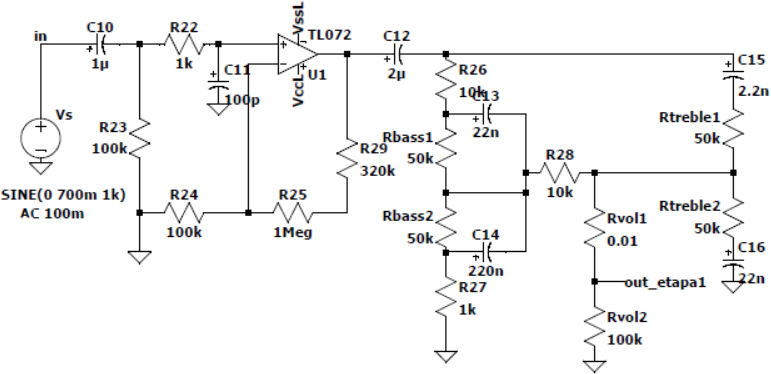
\includegraphics[width=0.75 \textwidth]{img/circuito/pre_amplificador.PNG}
    \caption{Circuito pre-amplificador.}
    \label{fig:ciruito_pre}
\end{figure}

\subsection{Fuente \textit{Switching}}

\par El circuito amplificador se alimenta con 4 tensiones diferentes, las cuales son $+35 \si[per-mode=symbol]{\volt}$, $+15 \si[per-mode=symbol]{\volt}$, $-35 \si[per-mode=symbol]{\volt}$ y $-15V$, para ello se diseñaron dos fuentes switching, una \textit{step down} para bajar de $35 \si[per-mode=symbol]{\volt}$ a $15 \si[per-mode=symbol]{\volt}$ y una \textit{step up} para subir de $-35 \si[per-mode=symbol]{\volt}$ a $-15 \si[per-mode=symbol]{\volt}$.\\

\par A partir de las hojas de datos de los reguladores \textbf{LM2576} y \textbf{LM2577}, en configuraciones indicadas para entregar las alimentaciones correspondientes. Se implementaron los siguientes circuitos tomados de las hojas de datos:\\

\vfill

\clearpage

\begin{figure}[H]
    \centering
    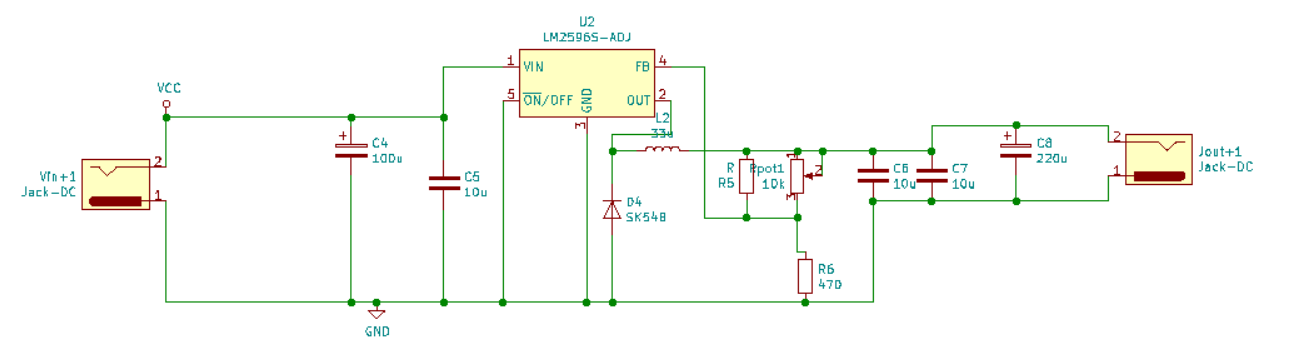
\includegraphics[width=0.95 \textwidth]{img/fuente/fuente_kicad_down.png}
    \caption{Circuito \textit{Step Down}.}
    \label{fig:step_down}
\end{figure}

\begin{figure}[H]
    \centering
    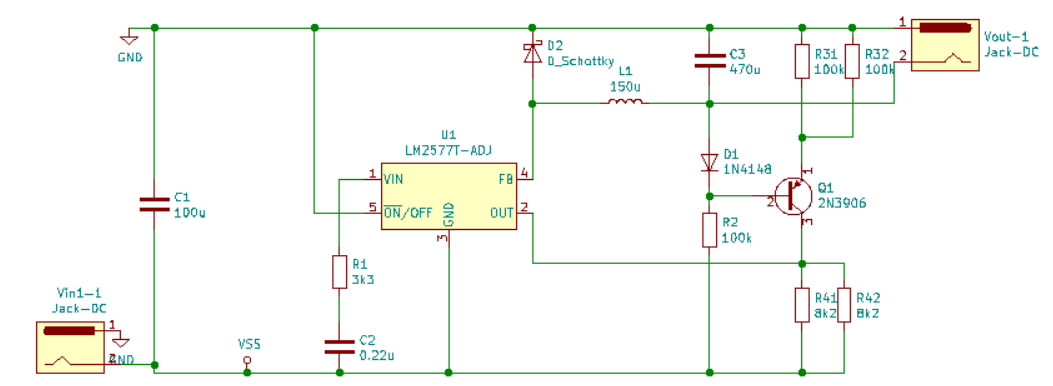
\includegraphics[width=0.95 \textwidth]{img/fuente/fuente_kicad_up.png}
    \caption{Circuito \textit{Step Up}.}
    \label{fig:step_up}
\end{figure}

\par Luego se diseñó el PCB de la fuente \textit{Switching} en \textit{Kicad} a partir de los circuitos mencionados, el resultado se puede observar a continuación:\\


\vfill

\clearpage




\begin{figure}[H]
\centering
\begin{subfigure}{0.5\textwidth}
        \centering
    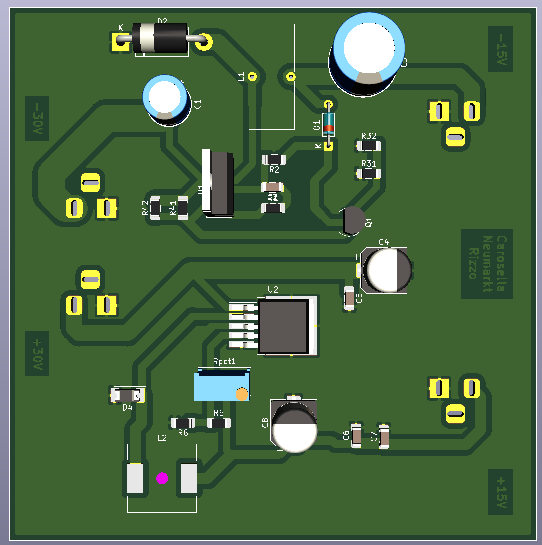
\includegraphics[width = 0.95 \textwidth]{img/fuente/fuente_switching_3D.PNG}
        \caption{Vista superior.}
        \label{fig::fuente_3D_T}
\end{subfigure}%
\begin{subfigure}{0.5\textwidth}
        \centering
    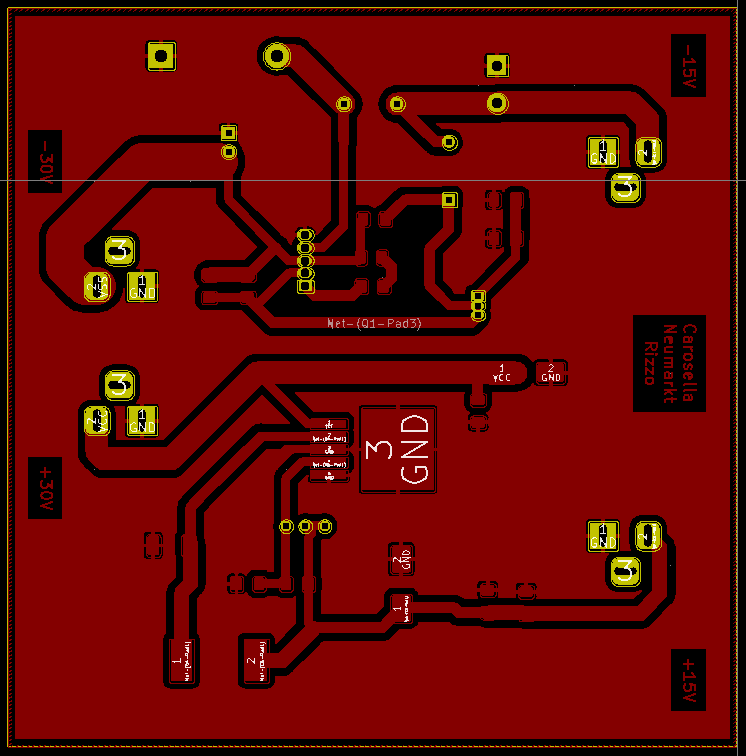
\includegraphics[width = 0.95 \textwidth]{img/fuente/fuente_switching.PNG}
        \caption{Vista inferior.}
        \label{fig::fuente_3D_B}
\end{subfigure}
\caption{Vista 3D del PCB de la fuente switching interna.}
\label{fig:fuente_3D}
\end{figure}



\subsection{Circuito amplificador}


\par A continuación, se muestran el esquemático del circuito implementado en \textit{Kicad}. En primer lugar, en la figura \figref{fig::ampli_kicad} muestra el amplificador principal clase G diseñado junto con el circuito de pre-amplificador. Luego se prosiguió por realizar el diseño del PCB. Para ello se aplicó un plano de masa en la capa superior de la placa. Por otro lado se utilizaron pistan anchas y cortas, de un espesor de $60 \si[per-mode=symbol]{\mils}$ a $118 \si[per-mode=symbol]{\mils}$ y separaciones entre pistas mayores a $12 \si[per-mode=symbol]{\mils}$. A continuación se muestran imágenes del PCB para el amplificador clase G a implementar:\\


\vfill

\clearpage



\begin{figure}[H]
        \centering
        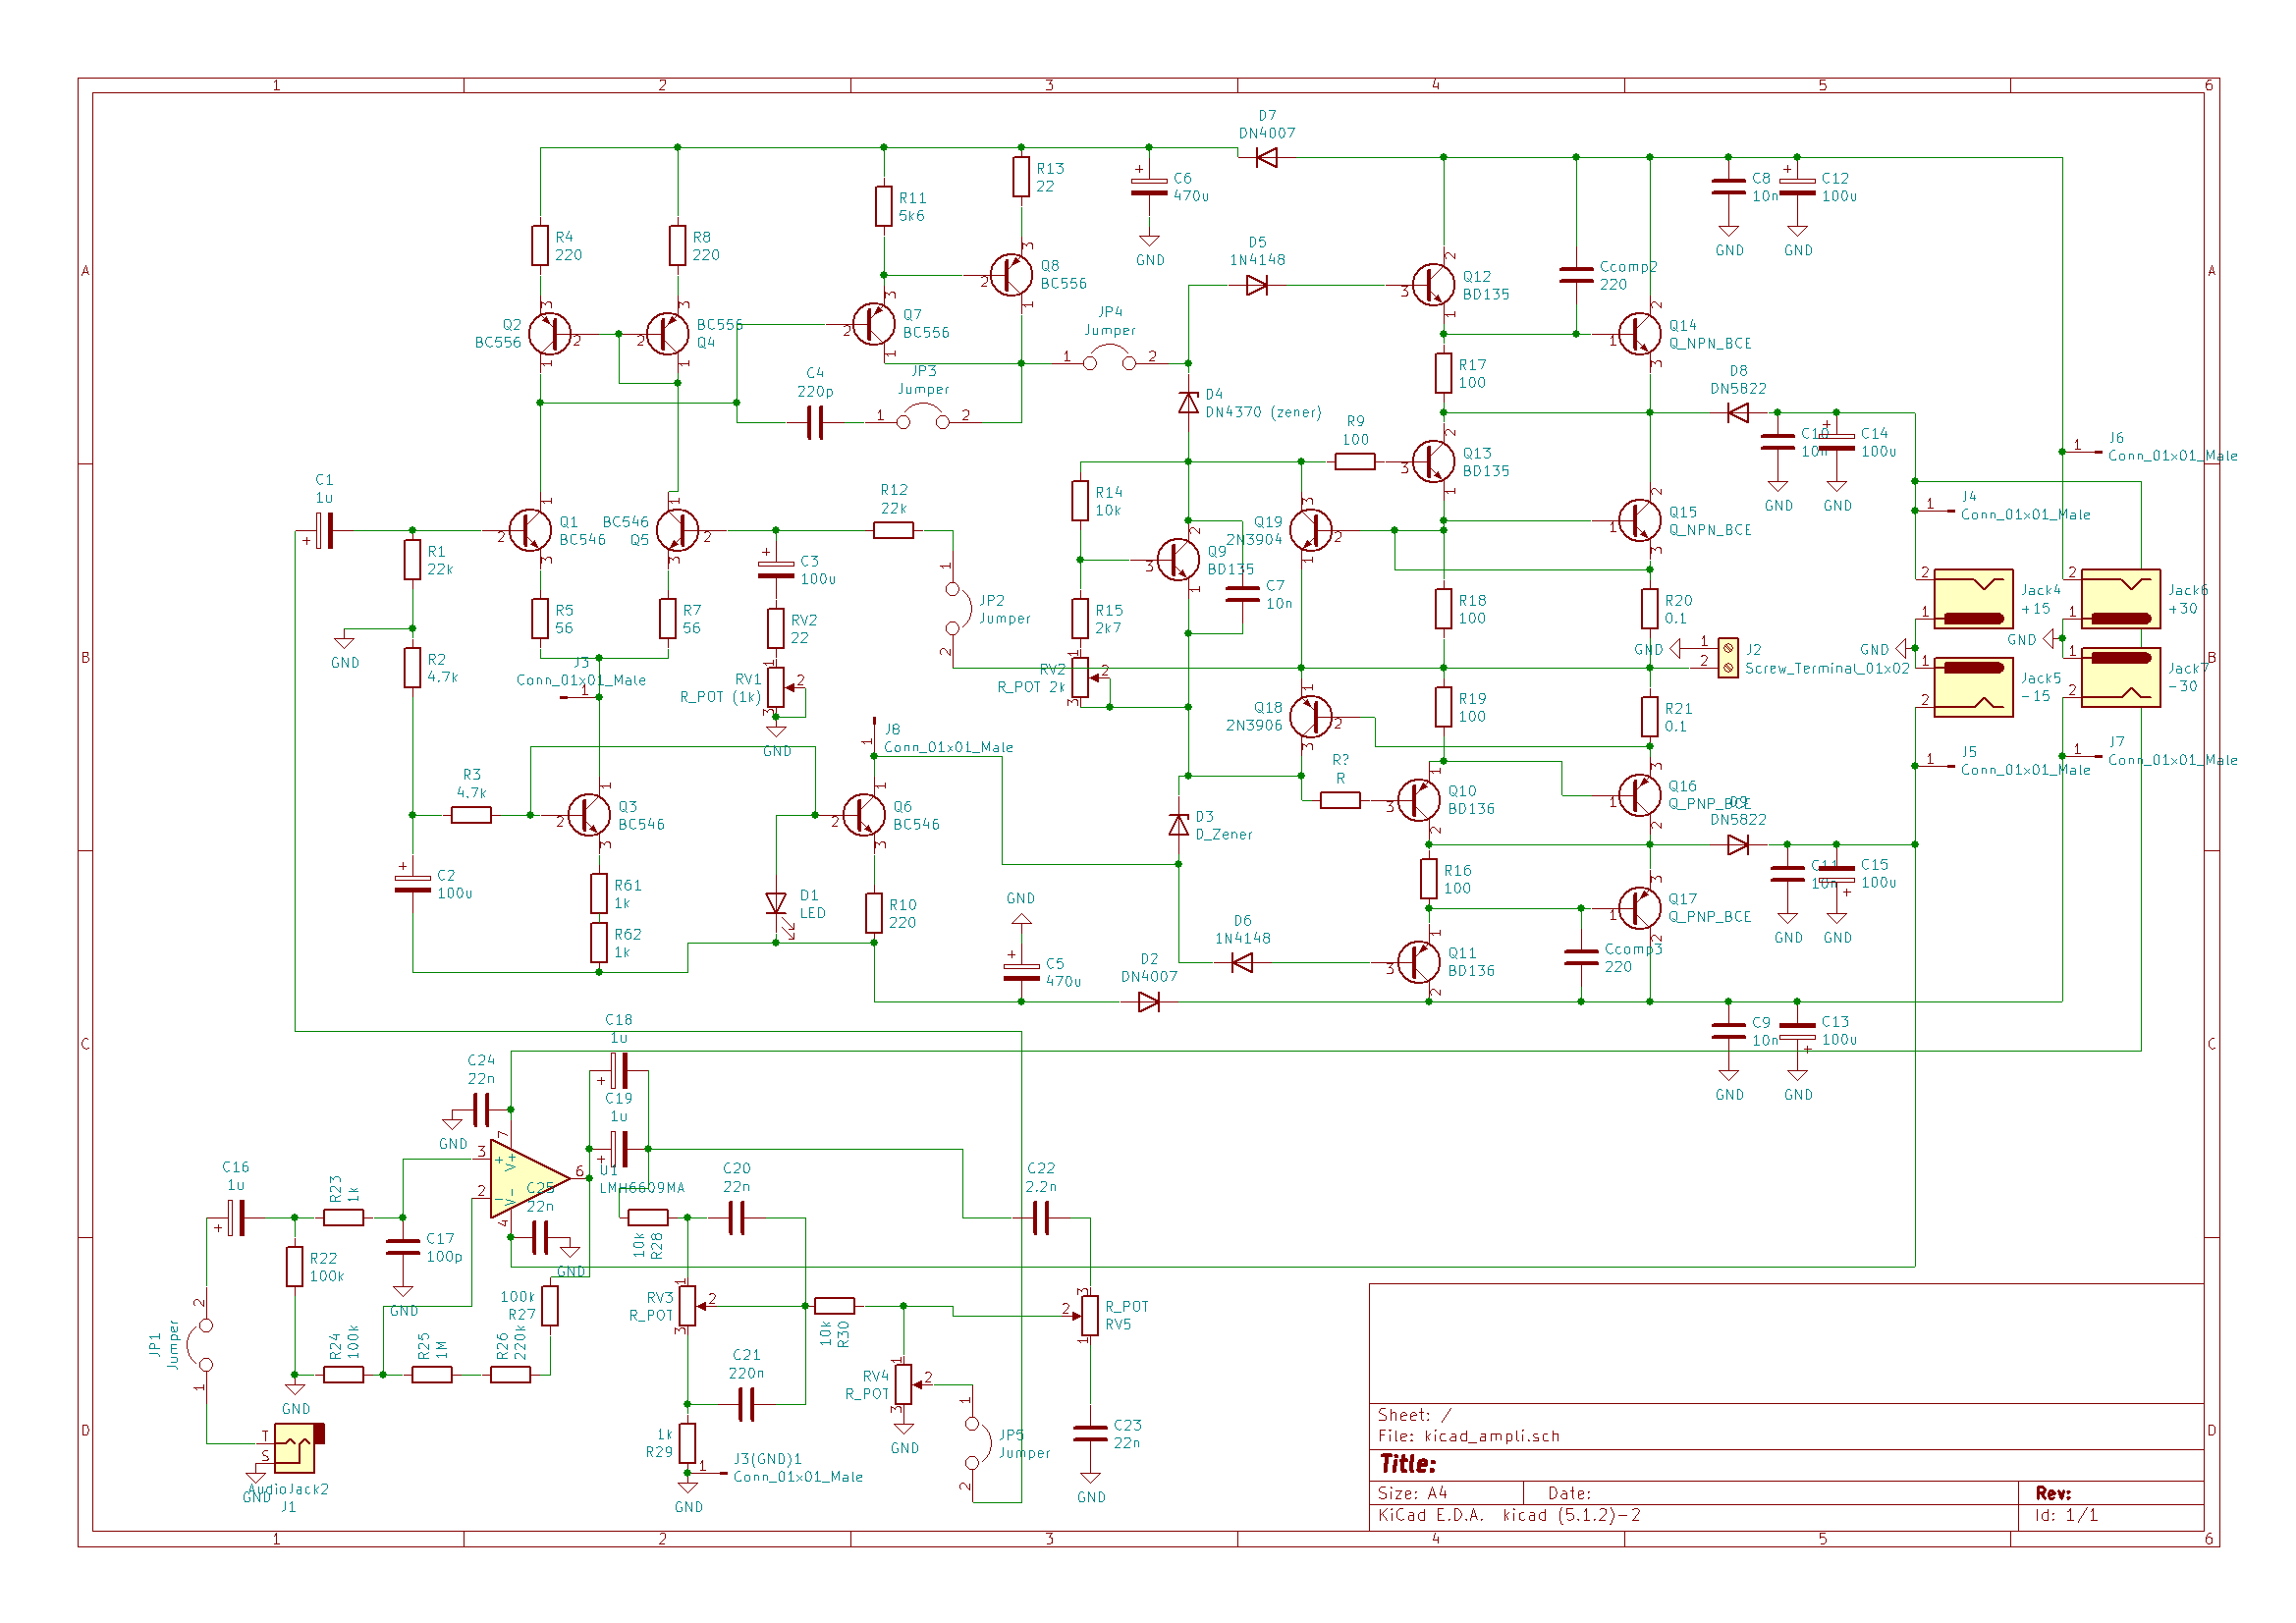
\includegraphics[height=0.85 \textwidth, angle=90]{img/circuito/kicad.png}
        \caption{Esquemático de amplificador con clase G.}
        \label{fig::ampli_kicad}
\end{figure}

\begin{figure}[H]
        \centering
        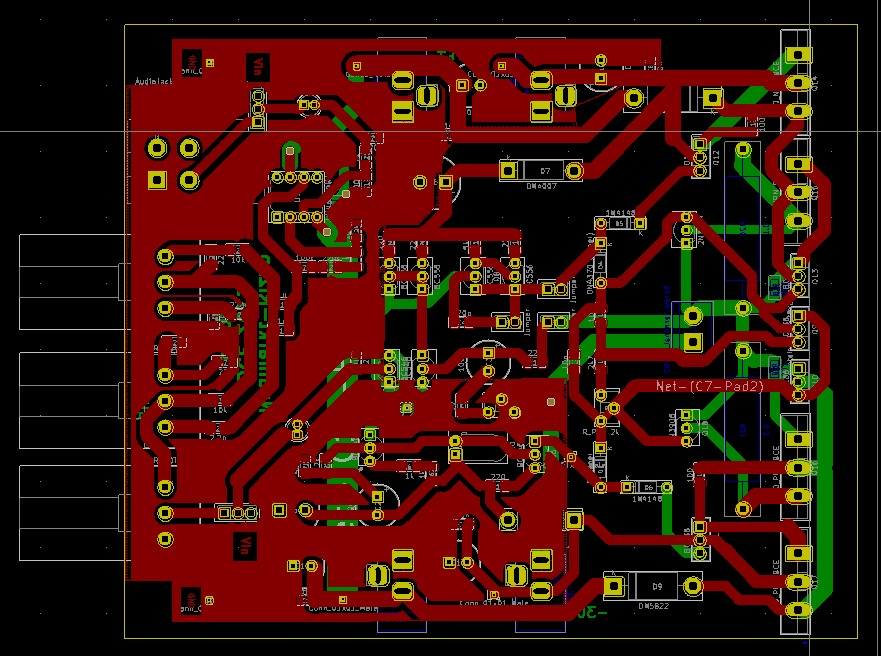
\includegraphics[width=0.65 \textwidth]{img/circuito/PCB1.jpeg}
        \caption{PCB del amplificador.}
        \label{fig::amp_PCB1}
\end{figure}


\begin{figure}[H]
\centering
\begin{subfigure}{0.5\textwidth}
        \centering
        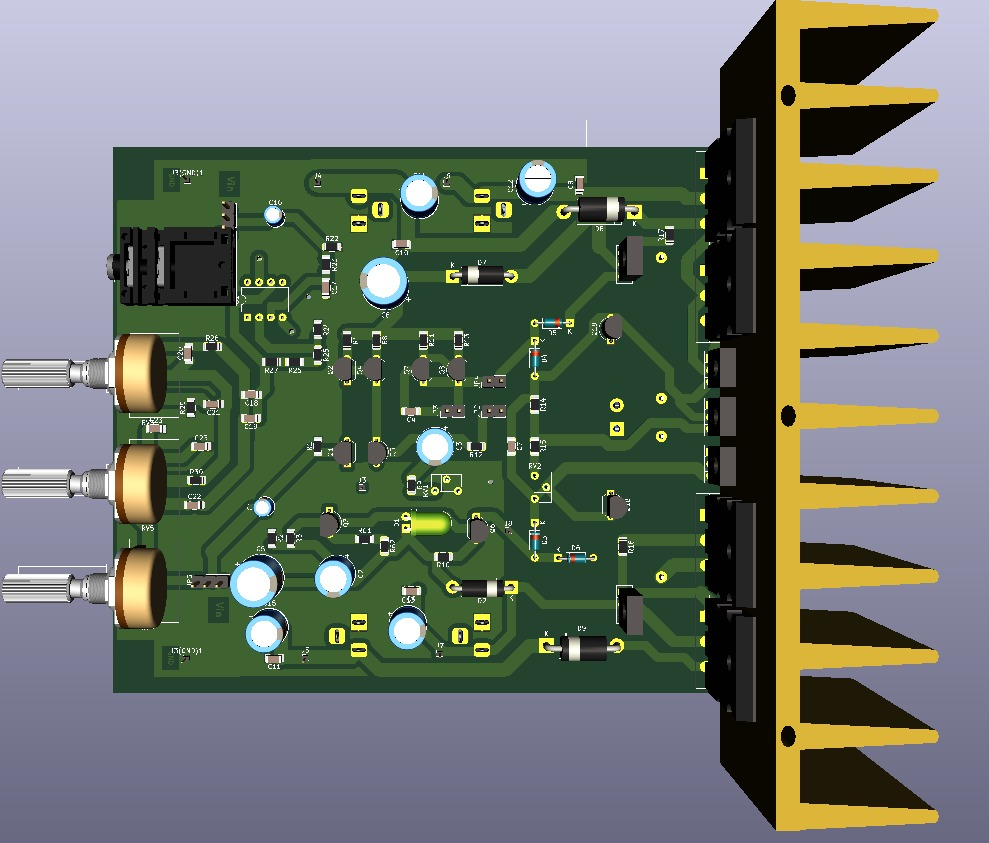
\includegraphics[width = 0.95 \textwidth]{img/circuito/PCB_3D_Top.jpeg}
        \caption{Vista superior.}
        \label{fig::PCB_3D_T}
\end{subfigure}%
\begin{subfigure}{0.5\textwidth}
        \centering
        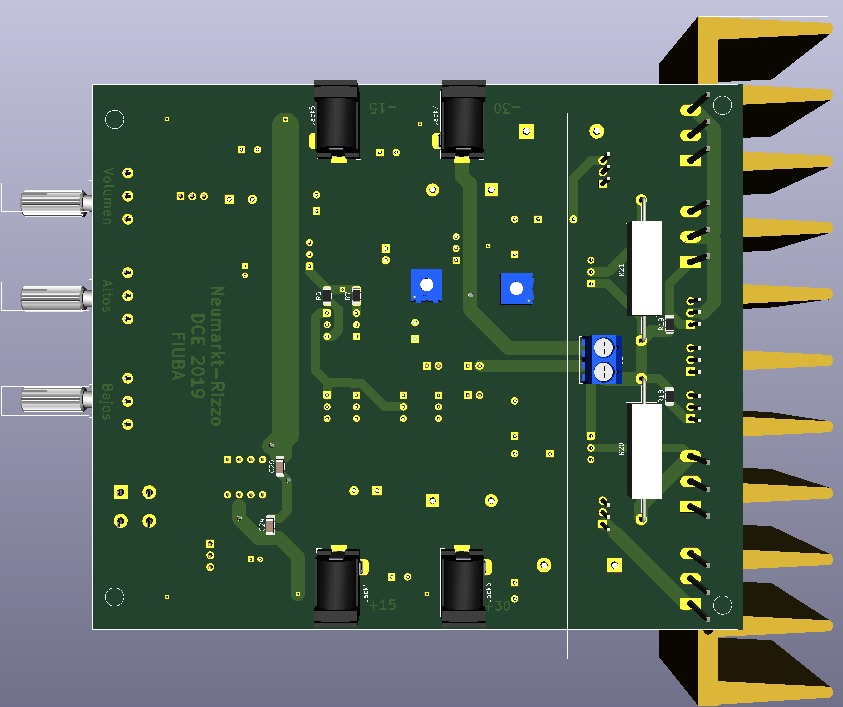
\includegraphics[width = 0.95 \textwidth]{img/circuito/PCB_3D_Bot.jpeg}
        \caption{Vista inferior.}
        \label{fig::PCB_3D_B}
\end{subfigure}
\caption{Vista 3D del PCB del amplificador.}
\label{fig:PCB_3D}
\end{figure}


\clearpage
%%\\\\\\\\\\\\\\\\\\\\\\\\\\\
%
%
%%\\\\\\\\\\\\\\\\\\\\\\\\\\\
\section{Simulaciones}
\resetallcounters

Todas las simulaciones se realizaron en \textbf{\textit{LTSPICE}}, pero dado que los gráficos de este programa no son muy buenos, los datos se exportaron a archivos de texto desde las opciones del programa, los mismos se cargaron y graficaron usando scripts de \textbf{\textit{MATLAB}}, estos gráficos son mas detallados y de mejor apariencia.\\


\subsection{Polarización}

\par Se simularon los valores en reposo de los transistores de la etapa amplificadora clase G, junto con la máxima potencia disipada en cada uno. Los resultados se muestran en el cuadro ~\tableref{table:PuntoQ_simulacion}\\

\begin{table}[H]  %%\centering
    
    \setlength\arrayrulewidth{1.5pt}
    \arrayrulecolor{white}
    \def\clinecolor{\hhline{|>{\arrayrulecolor{white}}-%
    >{\arrayrulecolor{white}}|-|-|-|-|-|}}
    
\begin{center}  
\resizebox{0.7 \textwidth}{!}{%    
\begin{tabularx}{1 \textwidth}%
    {|
    >{\columncolor{white} \centering\arraybackslash}m{0.3333\linewidth}
     |
    >{\columncolor{white} \centering\arraybackslash}m{0.1667\linewidth}
     |
    >{\columncolor{white} \centering\arraybackslash}m{0.1667\linewidth}
     |
    >{\columncolor{white} \centering\arraybackslash}m{0.1667\linewidth}
     |
    >{\columncolor{white} \centering\arraybackslash}m{0.1667\linewidth}
     |
    }
    \rowcolor{HeadersColor} \thead{Transistor} & \thead{$V_{BE_{Q}}$} & \thead{$V_{CE_{Q}}$} & \thead{$I_{C_{Q}}$} & \thead{ $P_{Q}$}\\    
    \hhline{|-|-|-|-|-|}
    %\rowcolor{Butter!20} \cellcolor{Butter!40} $I_{C}$ [$\si[per-mode=symbol]{\milli\ampere}$] & $0.54$ & $8.66$ & $9$ & $6$ & $5.5$ & $10$ & $10$  \\
    % \hhline{|-|-|-|-|-|}
    \rowcolor{gray!20} \cellcolor{gray!40} $Q_{1}$ (BC546C) & $612 \si[per-mode=symbol]{\milli\volt}$ & $33.87 \si[per-mode=symbol]{\volt}$ &  $549 \si[per-mode=symbol]{\micro\ampere}$ & $18.6 \si[per-mode=symbol]{\milli\watt}$ \\
    \hhline{|-|-|-|-|-|}
    \rowcolor{gray!20} \cellcolor{gray!40} $Q_{2}$ (BC556B) & $-610 \si[per-mode=symbol]{\milli\volt} $ & $-1.31\si[per-mode=symbol]{\volt}$  & $549 \si[per-mode=symbol]{\micro\ampere} $ & $722\si[per-mode=symbol]{\micro\watt}$ \\
    \hhline{|-|-|-|-|-|}
    \rowcolor{gray!20} \cellcolor{gray!40} $Q_{3}$ (BC546B) & $631\si[per-mode=symbol]{\milli\volt}$ & $31.78\si[per-mode=symbol]{\volt}$  & $1.1 \si[per-mode=symbol]{\milli\ampere} $ & $35\si[per-mode=symbol]{\milli\watt} $ \\
    \hhline{|-|-|-|-|-|}
    \rowcolor{gray!20} \cellcolor{gray!40} $Q_{4}$ (BC556B) & $-610\si[per-mode=symbol]{\milli\volt}$ & $33.78\si[per-mode=symbol]{\volt}$  & $549 \si[per-mode=symbol]{\micro\ampere} $ & $334\si[per-mode=symbol]{\milli\watt}$ \\
    \hhline{|-|-|-|-|-|}
    \rowcolor{gray!20} \cellcolor{gray!40} $Q_{5}$ (BC546B) & $612\si[per-mode=symbol]{\milli\volt}$ & $34.6\si[per-mode=symbol]{\volt}$  & $549 \si[per-mode=symbol]{\micro\ampere} $ & $19\si[per-mode=symbol]{\milli\watt} $ \\
    \hhline{|-|-|-|-|-|}
    \rowcolor{gray!20} \cellcolor{gray!40} $Q_{6}$ (BC546B) & $693\si[per-mode=symbol]{\milli\volt}$ & $28.8\si[per-mode=symbol]{\volt}$  & $9.71 \si[per-mode=symbol]{\milli\ampere} $ & $280\si[per-mode=symbol]{\milli\watt}$ \\
    \hhline{|-|-|-|-|-|}
    \rowcolor{gray!20} \cellcolor{gray!40} $Q_{7}$ (BC556B) & $-557\si[per-mode=symbol]{\milli\volt}$ & $30\si[per-mode=symbol]{\volt}$  & $170\si[per-mode=symbol]{\micro\ampere}$ & $5\si[per-mode=symbol]{\milli\watt}$ \\
    \hhline{|-|-|-|-|-|}
    \rowcolor{gray!20} \cellcolor{gray!40} $Q_{8}$ (BC556B) & $-669\si[per-mode=symbol]{\milli\volt}$ & $30.71\si[per-mode=symbol]{\volt}$  & $9.57\si[per-mode=symbol]{\milli\ampere}$ & $294\si[per-mode=symbol]{\milli\watt}$ \\ 
    \hhline{|-|-|-|-|-|}
    \rowcolor{gray!20} \cellcolor{gray!40} $Q_{9}$ (BD135) & $676\si[per-mode=symbol]{\milli\volt}$ & $2.96\si[per-mode=symbol]{\volt}$  & $9.40\si[per-mode=symbol]{\milli\ampere}$ & $28\si[per-mode=symbol]{\milli\watt} $ \\
    \hhline{|-|-|-|-|-|}
    \rowcolor{gray!20} \cellcolor{gray!40} $Q_{10}$(BD136) & $-722\si[per-mode=symbol]{\milli\volt}$ & $13.9\si[per-mode=symbol]{\volt}$  & $15\si[per-mode=symbol]{\milli\ampere} $ & $208\si[per-mode=symbol]{\milli\watt}$ \\
    \hhline{|-|-|-|-|-|}
    \rowcolor{gray!20} \cellcolor{gray!40} $Q_{11}$(BD136) & $10.95 \si[per-mode=symbol]{\volt} $ & $20.32\si[per-mode=symbol]{\volt}$  & $31\si[per-mode=symbol]{\pico\ampere} $ & $1.1\si[per-mode=symbol]{
ano\watt}$ \\
    \hhline{|-|-|-|-|-|}
    \rowcolor{gray!20} \cellcolor{gray!40} $Q_{12}$(BD135) & $-10.93 \si[per-mode=symbol]{\volt}$ & $20.32\si[per-mode=symbol]{\volt}$  & $31\si[per-mode=symbol]{\pico\ampere} $ & $1.1\si[per-mode=symbol]{
ano\watt}$ \\
    \hhline{|-|-|-|-|-|}
    \rowcolor{gray!20} \cellcolor{gray!40} $Q_{13}$(BD135) & $693\si[per-mode=symbol]{\milli\volt}$ & $13.88\si[per-mode=symbol]{\volt}$  & $18.9\si[per-mode=symbol]{\milli\ampere}$ & $263\si[per-mode=symbol]{\milli\watt}$ \\
    \hhline{|-|-|-|-|-|}
    \rowcolor{gray!20} \cellcolor{gray!40} $Q_{14}$(MJL21194) & $1.04 \si[per-mode=symbol]{\nano\volt} $ & $20.32\si[per-mode=symbol]{\volt}$  & $26\si[per-mode=symbol]{\pico\ampere} $ & $522\si[per-mode=symbol]{\pico\watt}$ \\
    \hhline{|-|-|-|-|-|}
    \rowcolor{gray!20} \cellcolor{gray!40} $Q_{15}$(MJL21194) & $722\si[per-mode=symbol]{\milli\volt}$ & $14.6\si[per-mode=symbol]{\volt}$  & $714\si[per-mode=symbol]{\milli\ampere}$ & $10.43 \si[per-mode=symbol]{\watt} $ \\
    \hhline{|-|-|-|-|-|}
    \rowcolor{gray!20} \cellcolor{gray!40} $Q_{16}$(MJL21193) & $-678\si[per-mode=symbol]{\milli\volt}$ & $14.6\si[per-mode=symbol]{\volt}$  & $718\si[per-mode=symbol]{\milli\ampere}$ & $10.49 \si[per-mode=symbol]{\watt} $ \\
    \hhline{|-|-|-|-|-|}
    \rowcolor{gray!20} \cellcolor{gray!40} $Q_{17}$(MJL21193) & $-986\si[per-mode=symbol]{\milli\volt}$ & $20.32\si[per-mode=symbol]{\volt}$  & $1.76\si[per-mode=symbol]{\pico\ampere}$ & $459\si[per-mode=symbol]{\pico\watt}$ \\
    \hhline{|-|-|-|-|-|}
    \rowcolor{gray!20} \cellcolor{gray!40} $Q_{18}$(2N3906) & $-72\si[per-mode=symbol]{\milli\volt}$ & $1.47\si[per-mode=symbol]{\volt}$  & $1.47\si[per-mode=symbol]{\pico\ampere}$ & $2.2\si[per-mode=symbol]{\pico\watt}$ \\
    \hhline{|-|-|-|-|-|}
    \rowcolor{gray!20} \cellcolor{gray!40} $Q_{19}$(2N3904) & $72\si[per-mode=symbol]{\milli\volt}$ & $1.48\si[per-mode=symbol]{\volt}$  & $1.58\si[per-mode=symbol]{\pico\ampere}$ & $2.3\si[per-mode=symbol]{\pico\watt}$ \\
    \hhline{|-|-|-|-|-|}            
    \end{tabularx}}
	\caption{\footnotesize{Punto de reposo de los transistores y máxima potencia disipada en operación.}}
	\label{table:PuntoQ_simulacion}
	\end{center}
\end{table}



\par En la figura ~\figref{fig:PuntoQ_simulacion} se pueden verificar los resultados de la simulación con las referencias en el circuito pertinente.

\vfill

\clearpage

\begin{figure}[H]
    \centering
    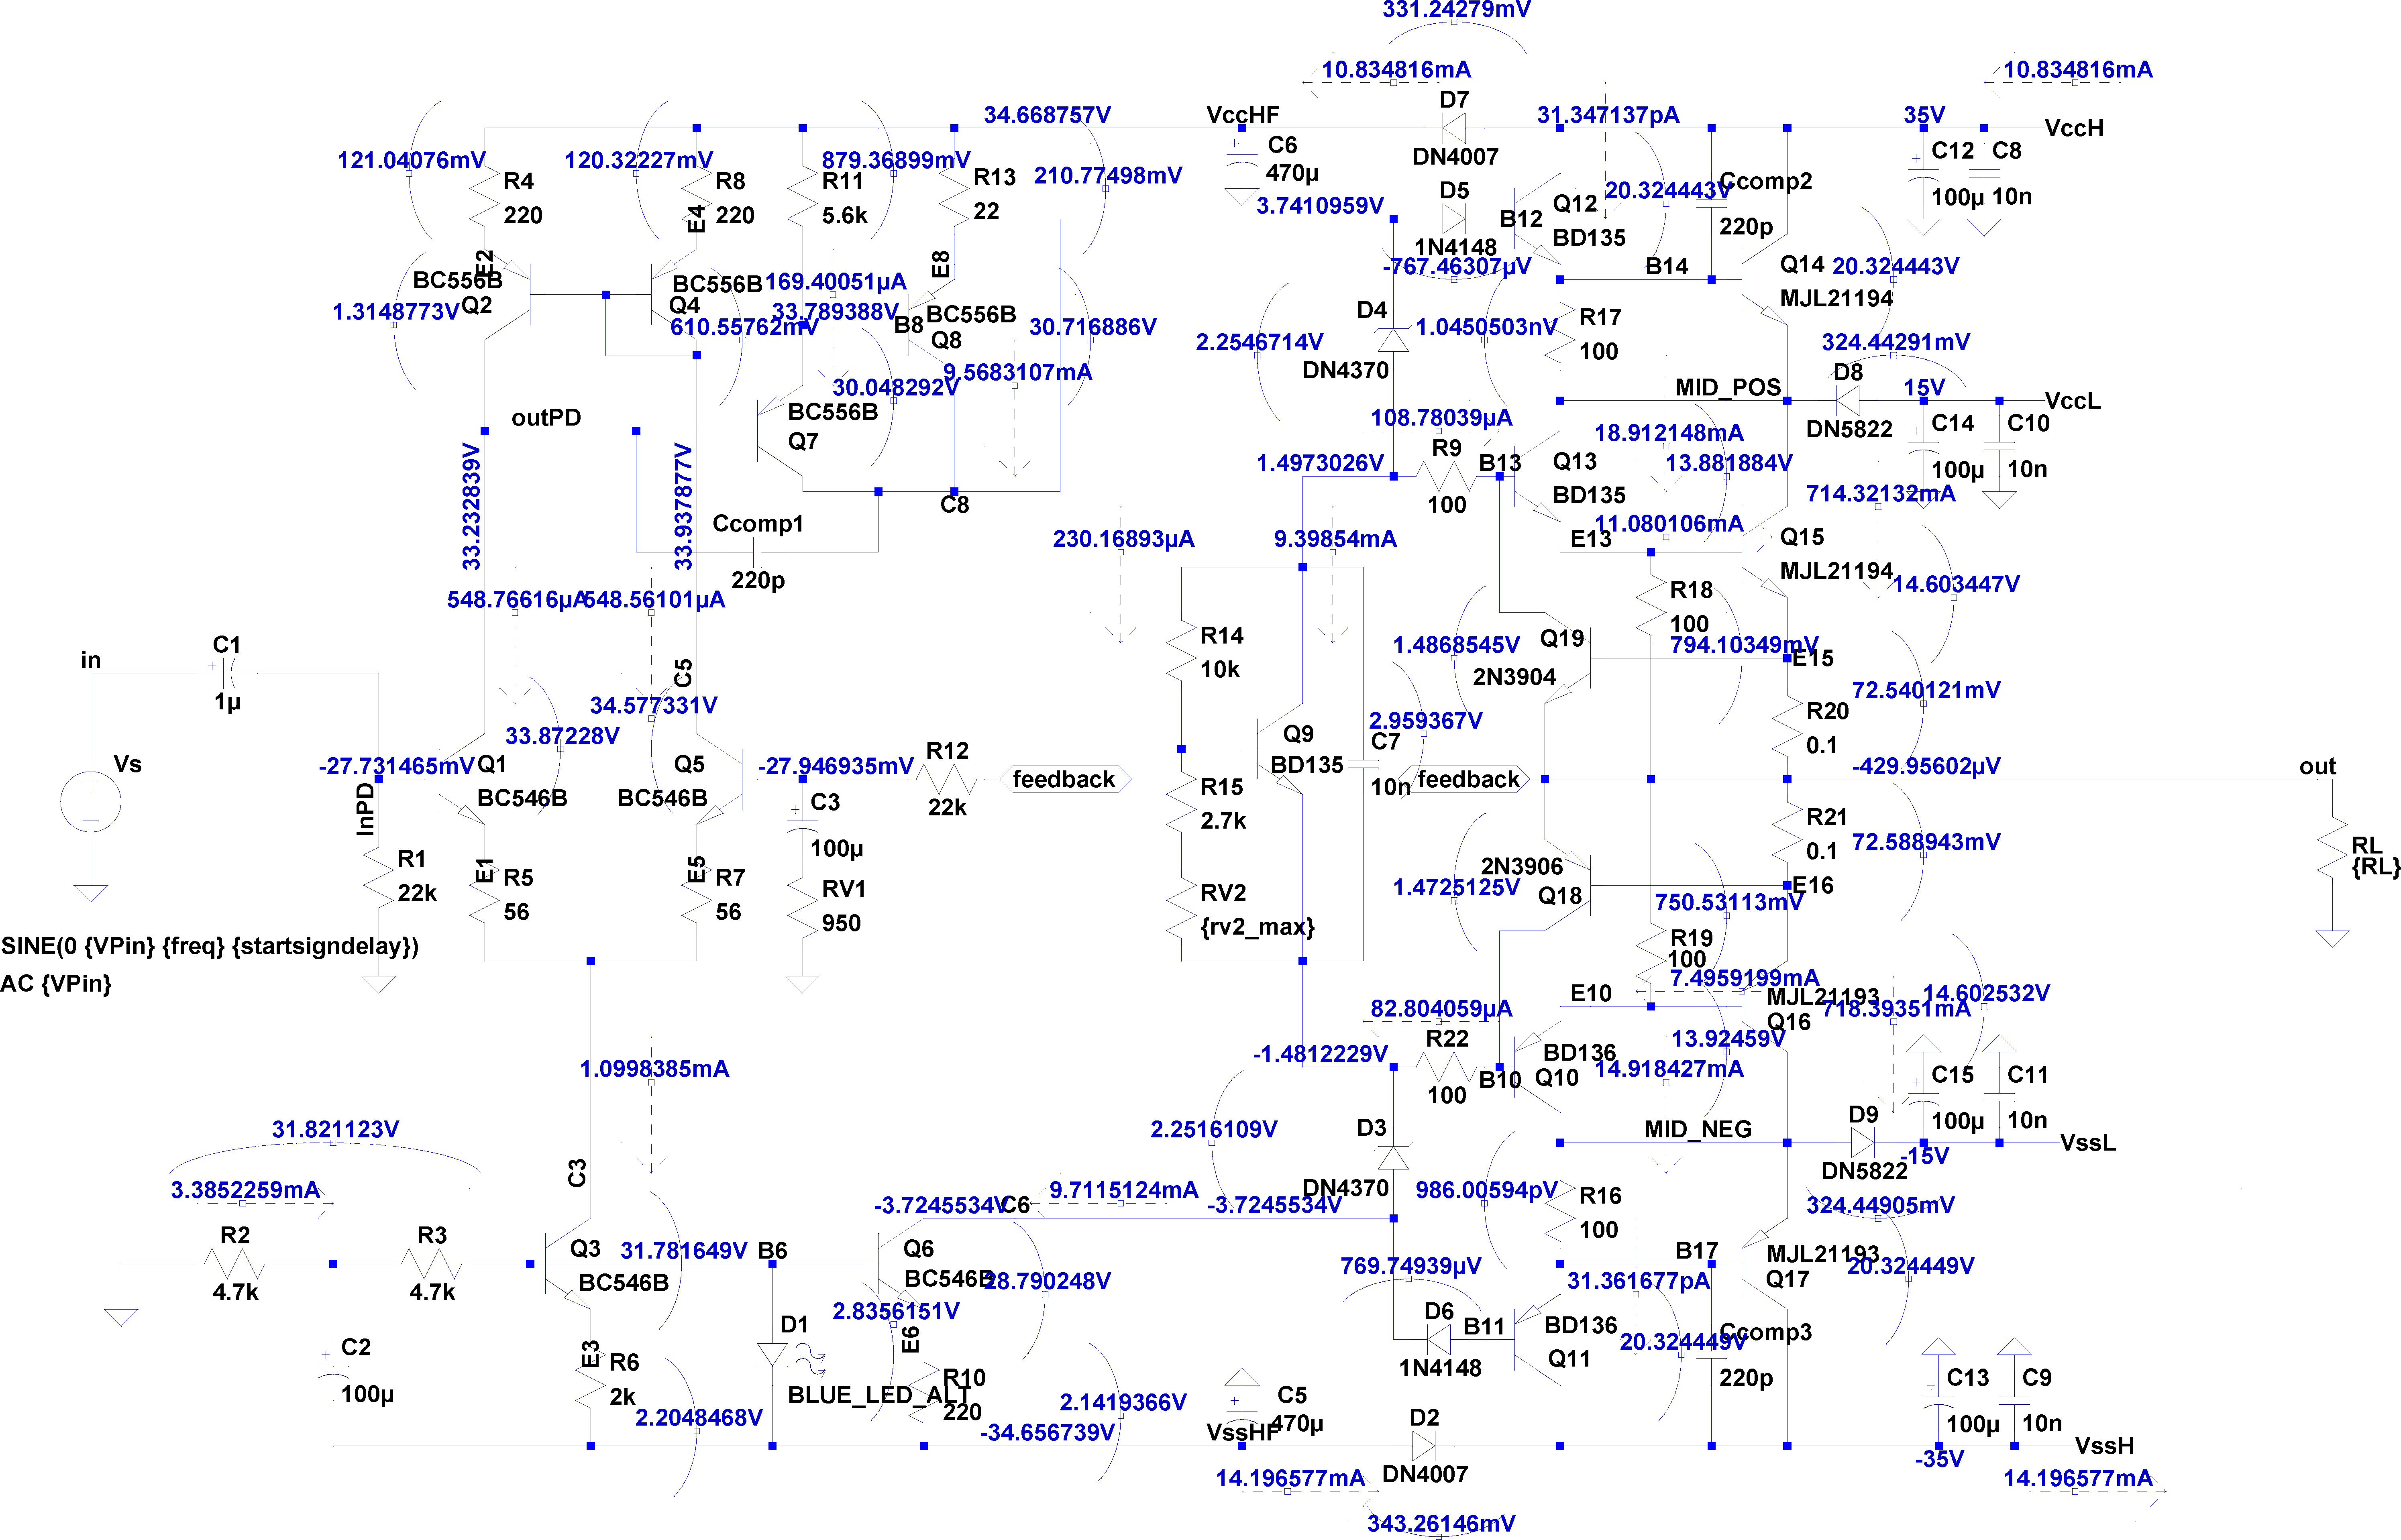
\includegraphics[height=0.77 \textwidth, angle=90]{./img/circuito/amplifier.png}
    \caption{Circuito simulado mostrando los valores de polarización.}
    \label{fig:PuntoQ_simulacion}
\end{figure}

\clearpage

\subsection{Ganancia de lazo}

\par En la figura ~\figref{fig:gain_loop_sim} se puede observar la ganancia de lazo del circuito, simulado a distintas frecuencias. A su vez, se especifica el margen de ganancia y de fase, para verificar la correcta estabilización del circuito. Obteniéndose de este modo:

\begin{itemize}
    \item Margen de ganancia: $29.21 \si[per-mode=symbol]{\decibel}$
    \item Margen de fase: $86.12 \si[per-mode=symbol]{\degree}$
\end{itemize}

\vfill

\clearpage

\begin{figure}[H]
    \centering
    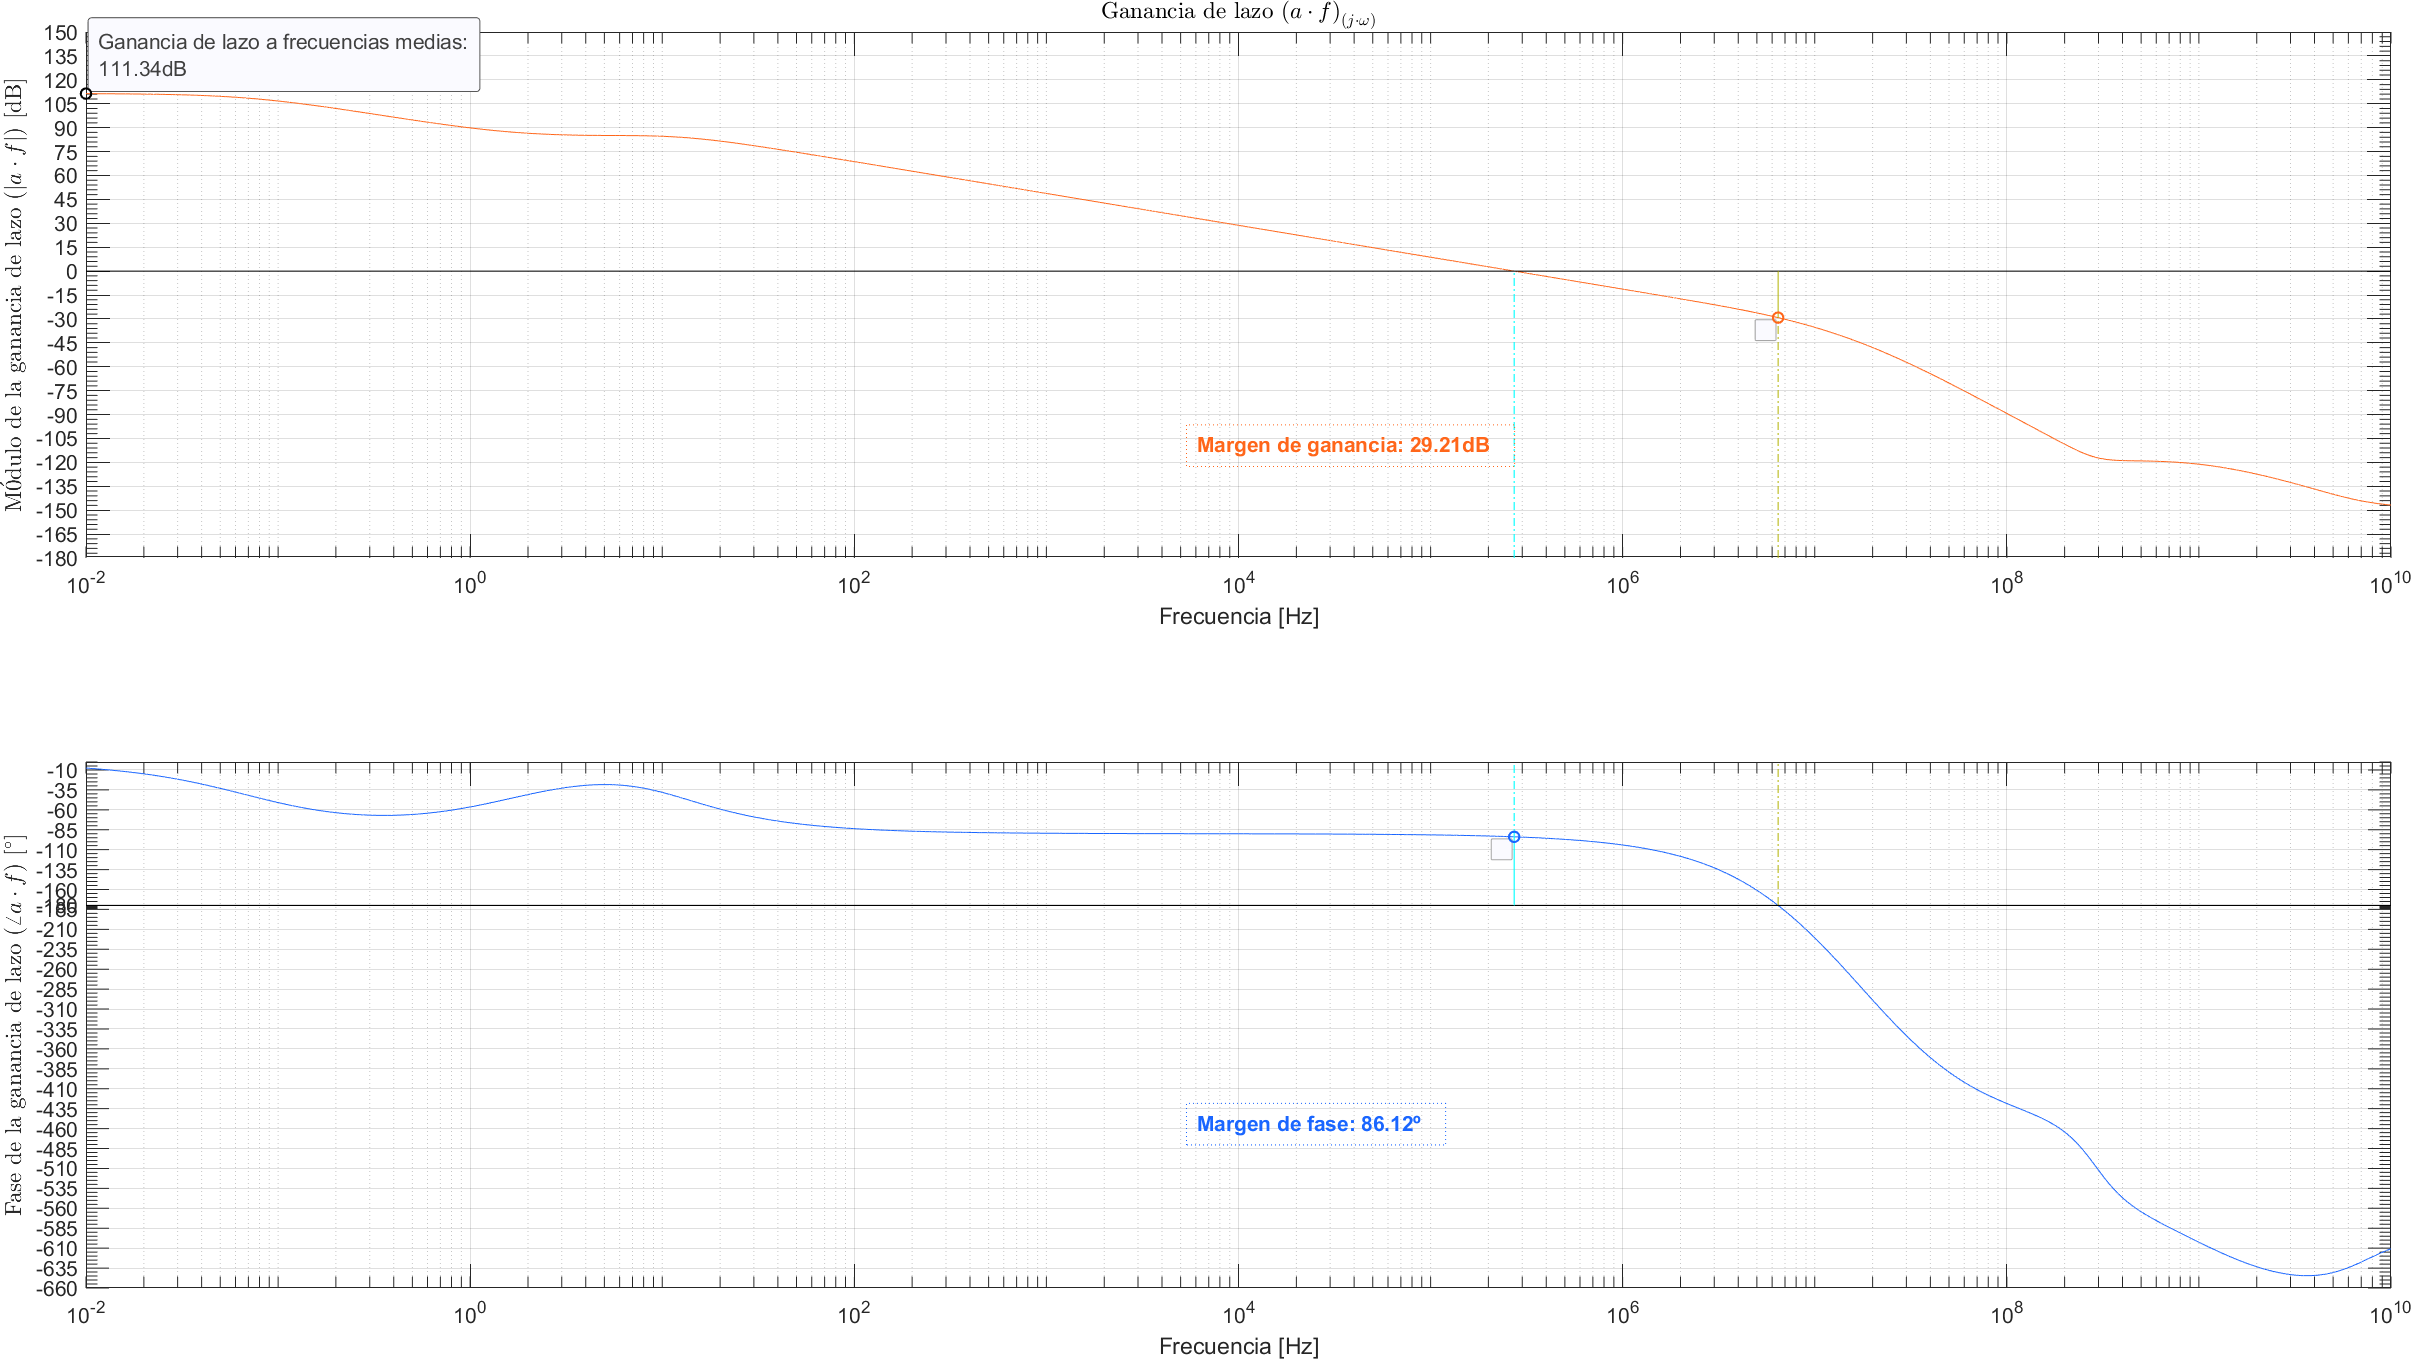
\includegraphics[height=0.66 \textwidth, angle=90]{./img/simulaciones/Loop/gain_loop.png}
    \caption{Ganancia de lazo (simulación).}
    \label{fig:gain_loop_sim}
\end{figure}

\clearpage

\subsection{Ancho de banda a baja potencia}

\par En la figura ~\figref{fig:Low_power_BW} se muestra el resultado de la simulación del ancho de banda del circuito.
\par Obtenemos un ancho de banda de $97.89kHz$ con frecuencias de corte:

\begin{itemize}
    \item $f_l =22.34 \si[per-mode=symbol]{\hertz}$
    \item $f_h =97.92 \si[per-mode=symbol]{\kilo\hertz}$
\end{itemize}

\vfill

\clearpage

\begin{figure}[H]
    \centering
    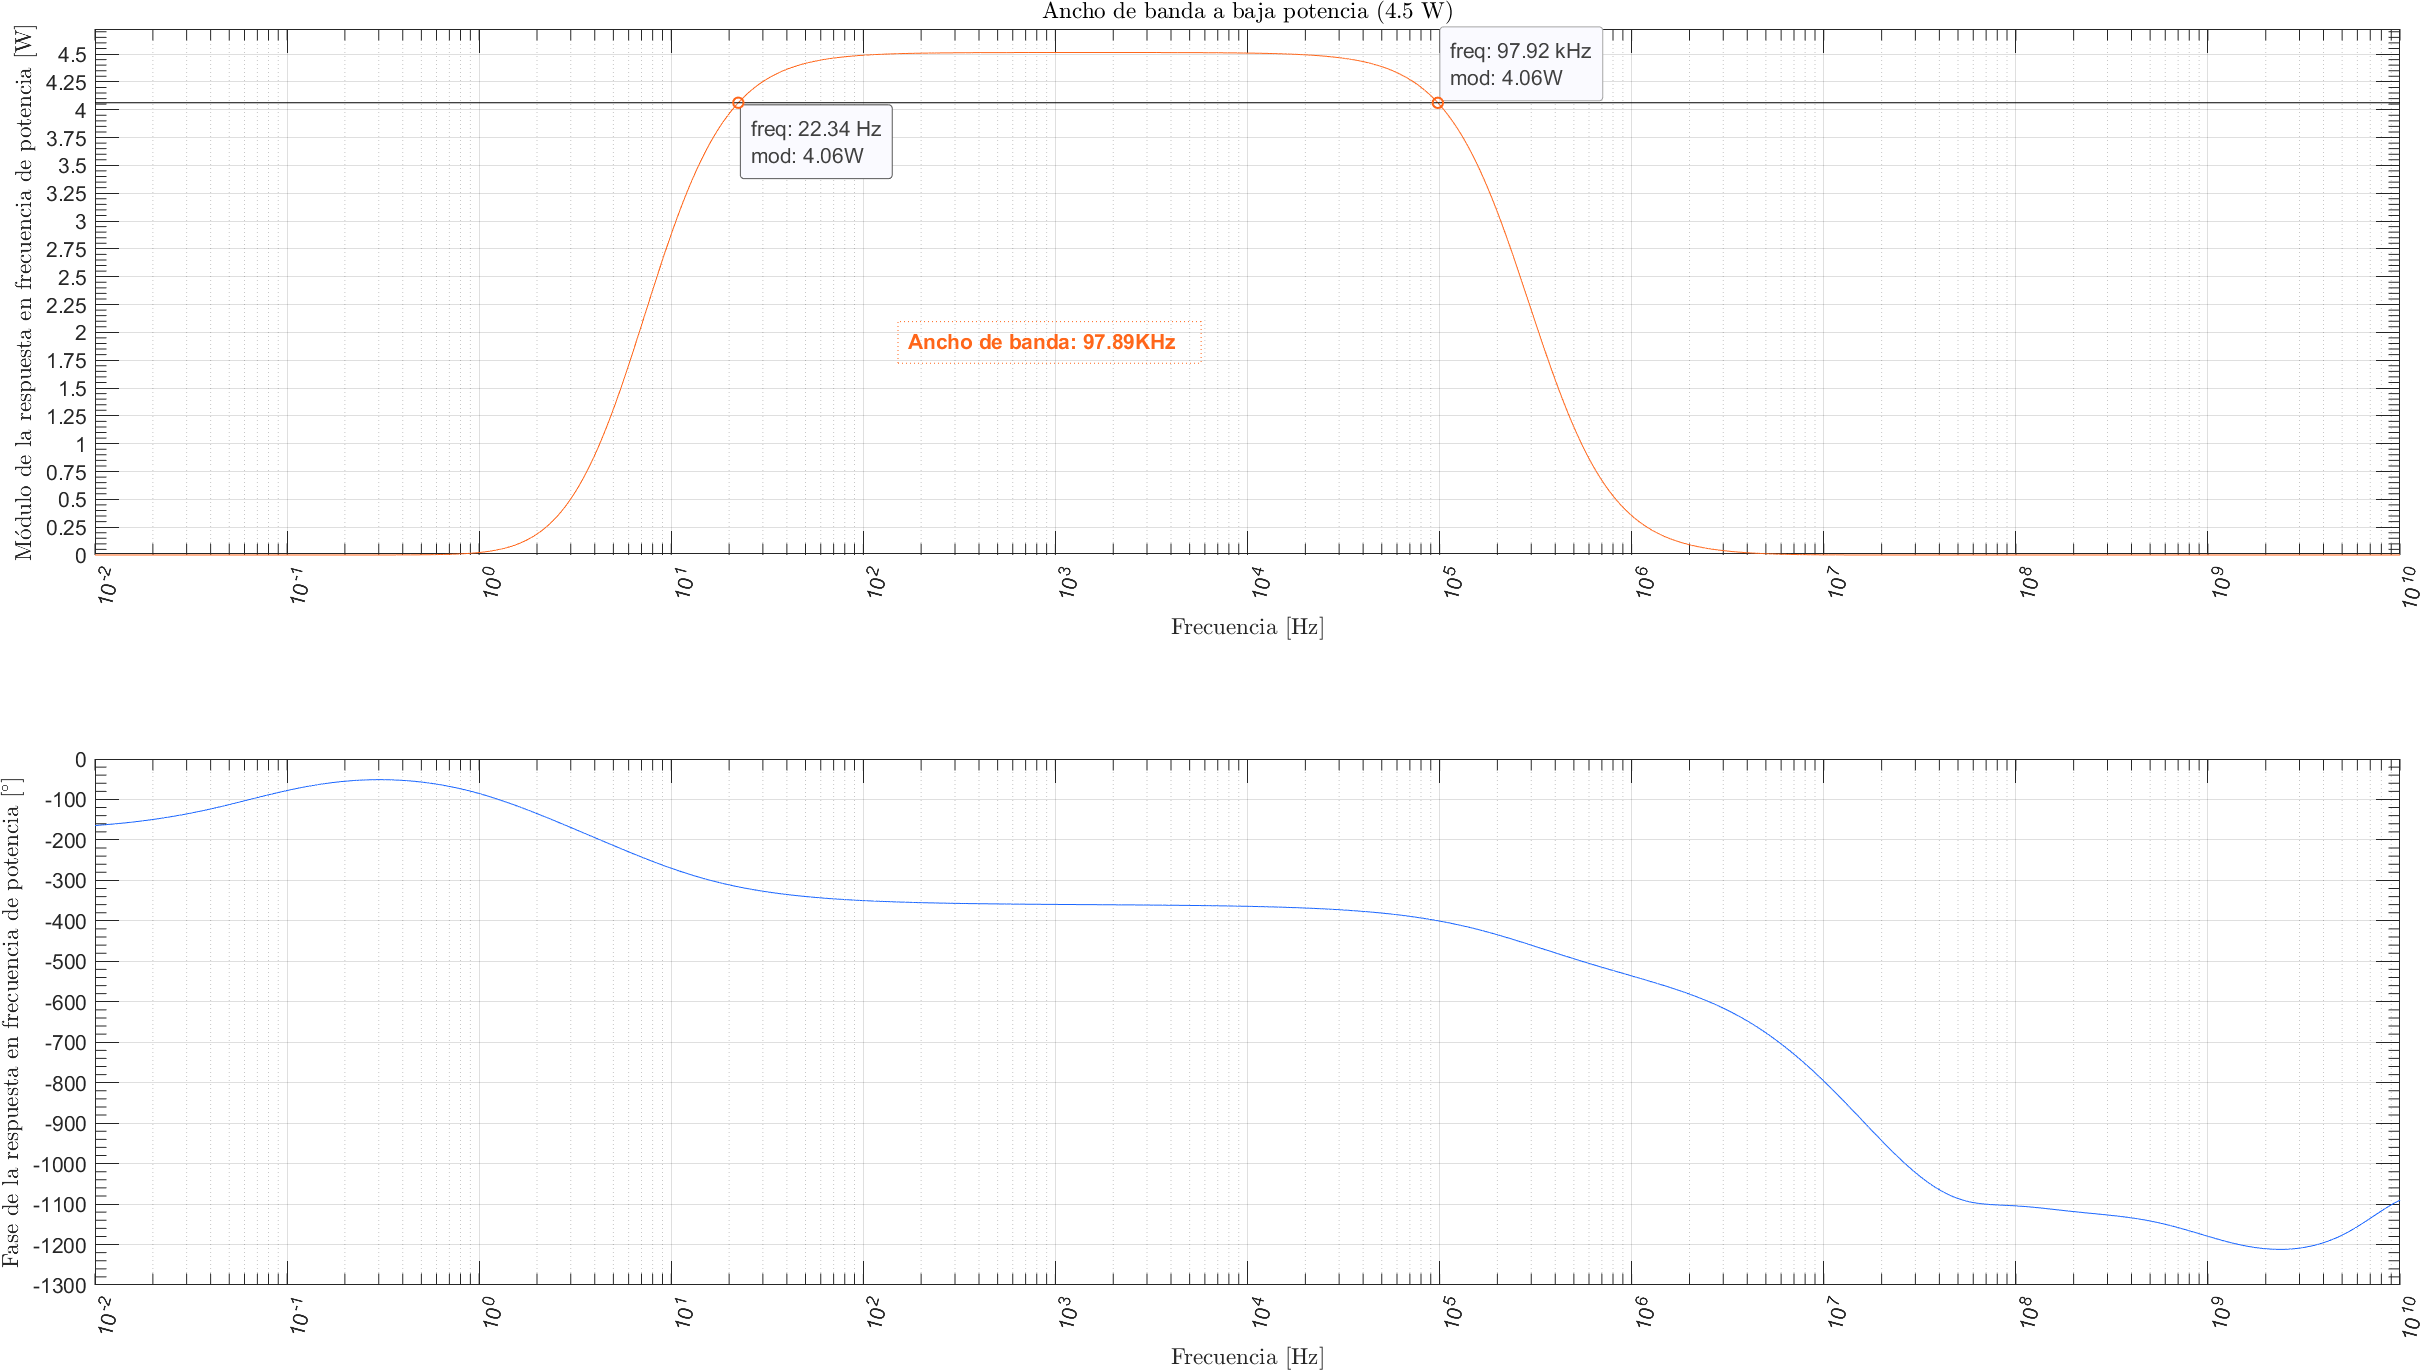
\includegraphics[height=0.66 \textwidth, angle=90]{./img/simulaciones/BW/Low_power_BW.png}    \caption{Ancho de banda a baja potencia (simulación).}
    \label{fig:Low_power_BW}
\end{figure}


\subsection{Ancho de banda de potencia}

\par En la figura ~\figref{fig:Power_BW_sim}, se observa el resultado de la simulación del ancho de banda de potencia simulado.
\par Obtenemos en el circuito un ancho de banda de potencia de $97.89kHz$ con frecuencias de corte:

\begin{itemize}
    \item $f_l = 22.34 \si[per-mode=symbol]{\hertz}$
    \item $f_h = 97.84 \si[per-mode=symbol]{\kilo\hertz}$
\end{itemize}

\vfill

\clearpage

\begin{figure}[H]
    \centering
    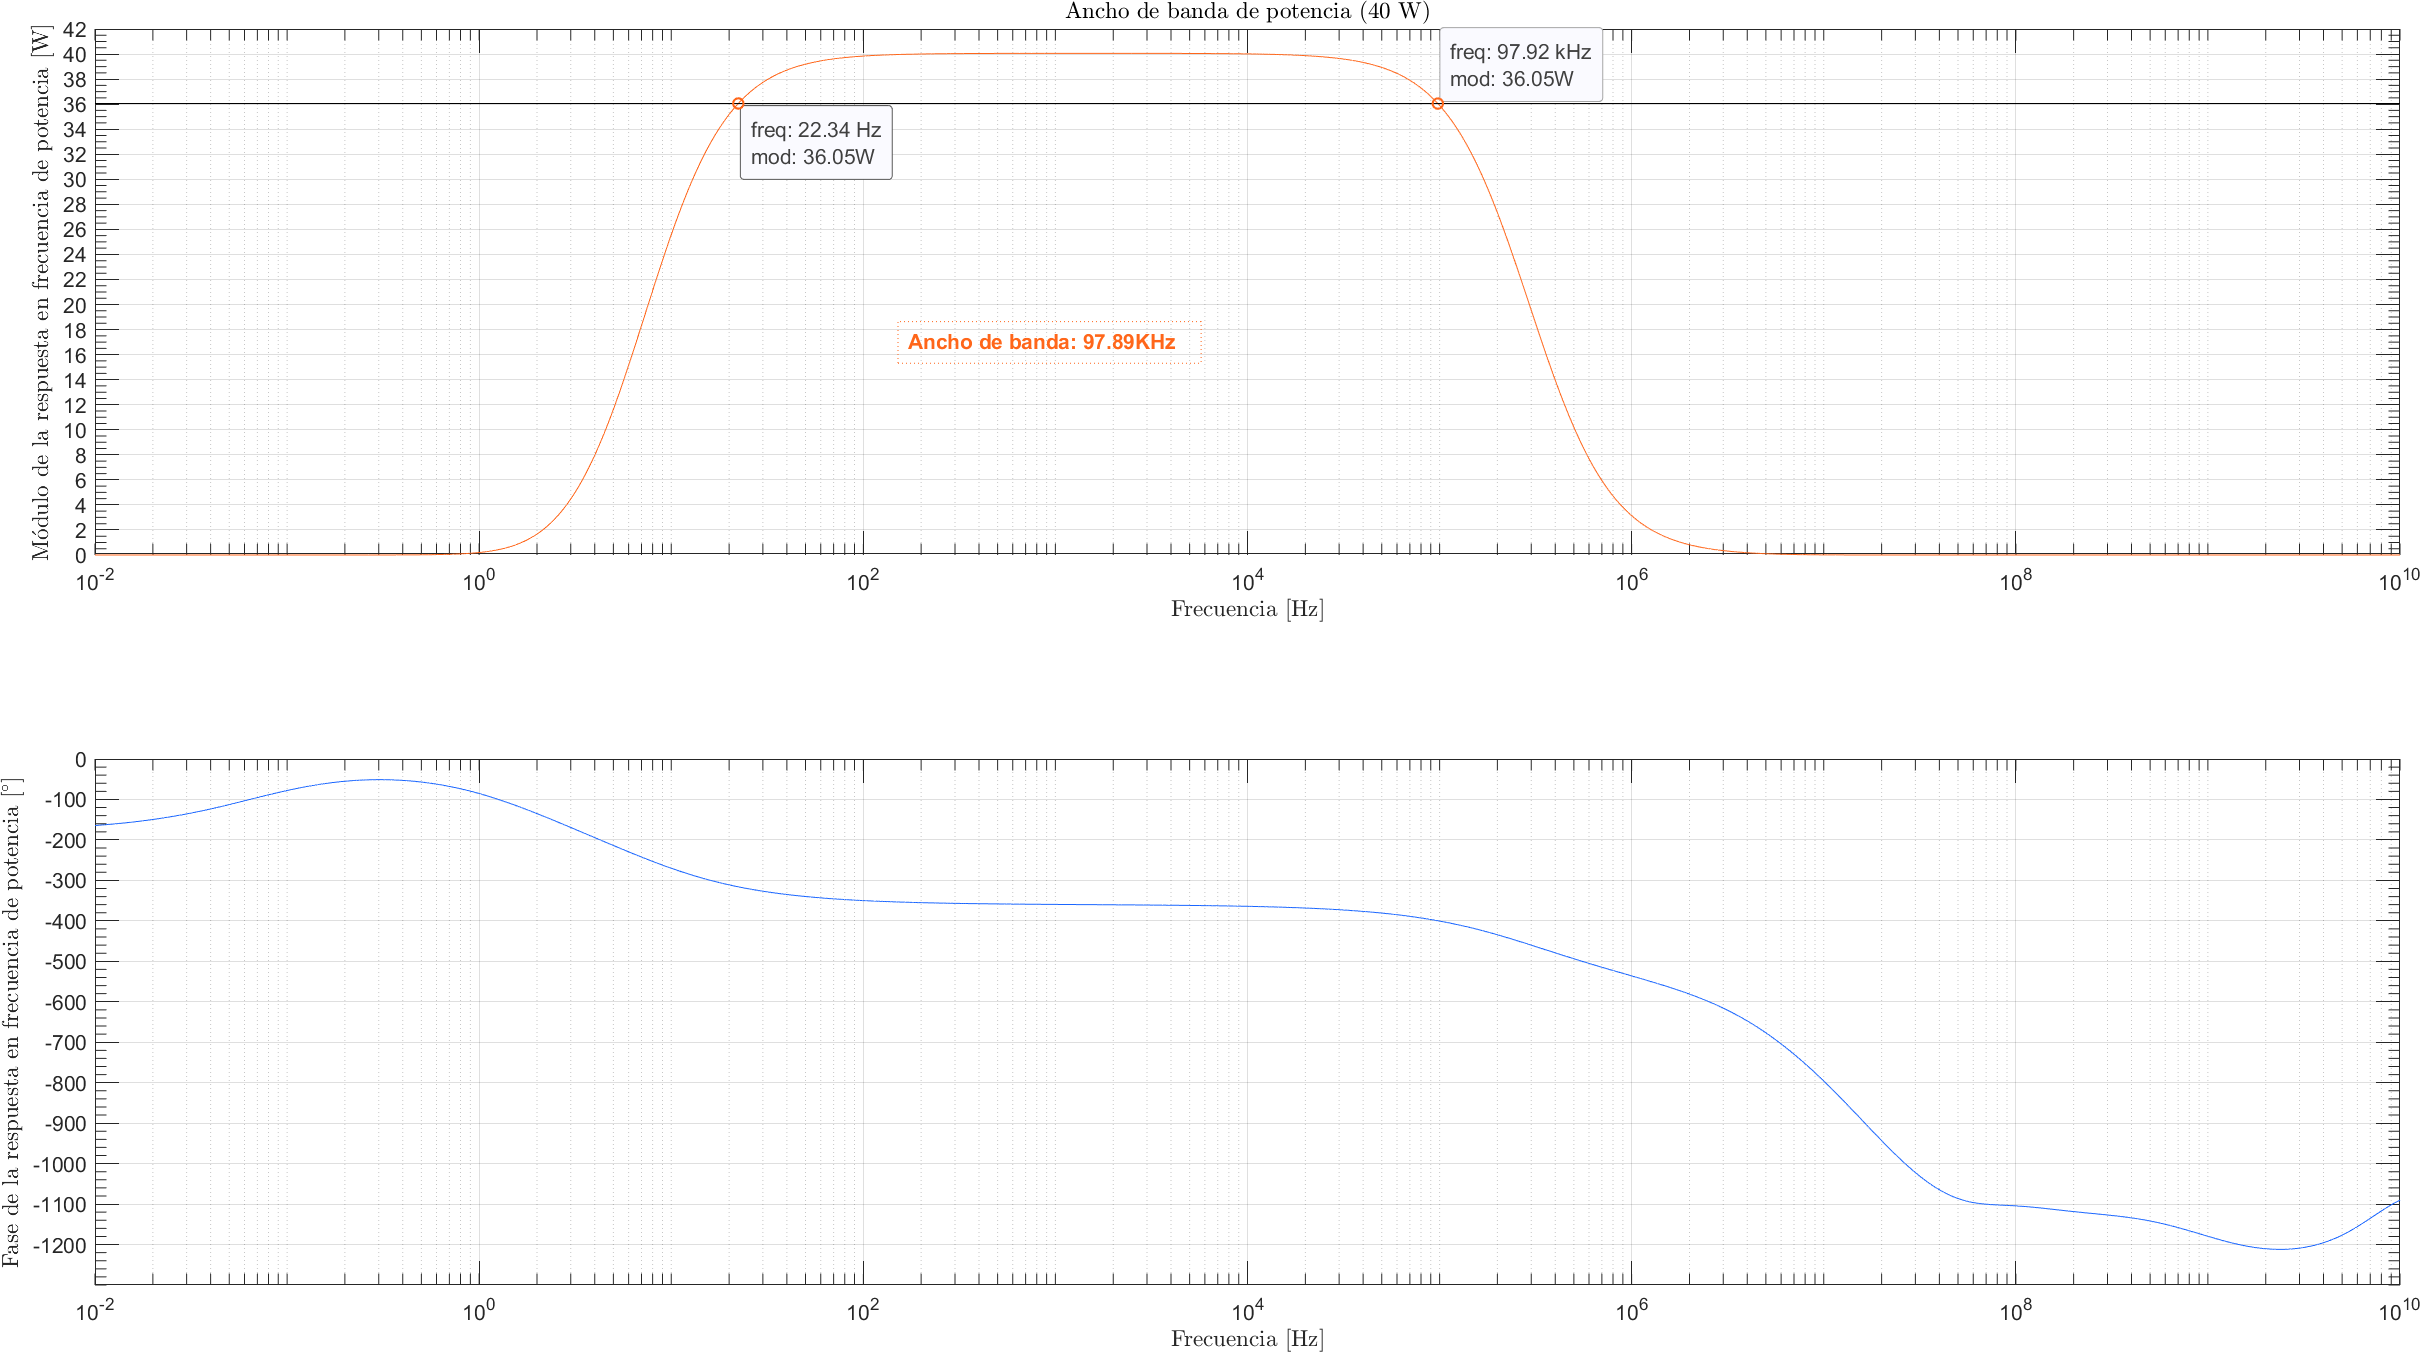
\includegraphics[height=0.66 \textwidth, angle=90]{./img/simulaciones/BW/Power_BW.png}
    \caption{Ancho de banda de potencia (simulación).}
    \label{fig:Power_BW_sim}
\end{figure}

\clearpage

\subsection{Impedancias de entrada y salida}

\par En las figuras ~\figref{fig:amplifier_Zi_sim} y ~\figref{fig:amplifier_Zo_sim} , se observa los valores de la resistencia de entrada y salida del amplificador, respectivamente, en función de la frecuencia.

\vfill

\clearpage

\begin{figure}[H]
    \centering
    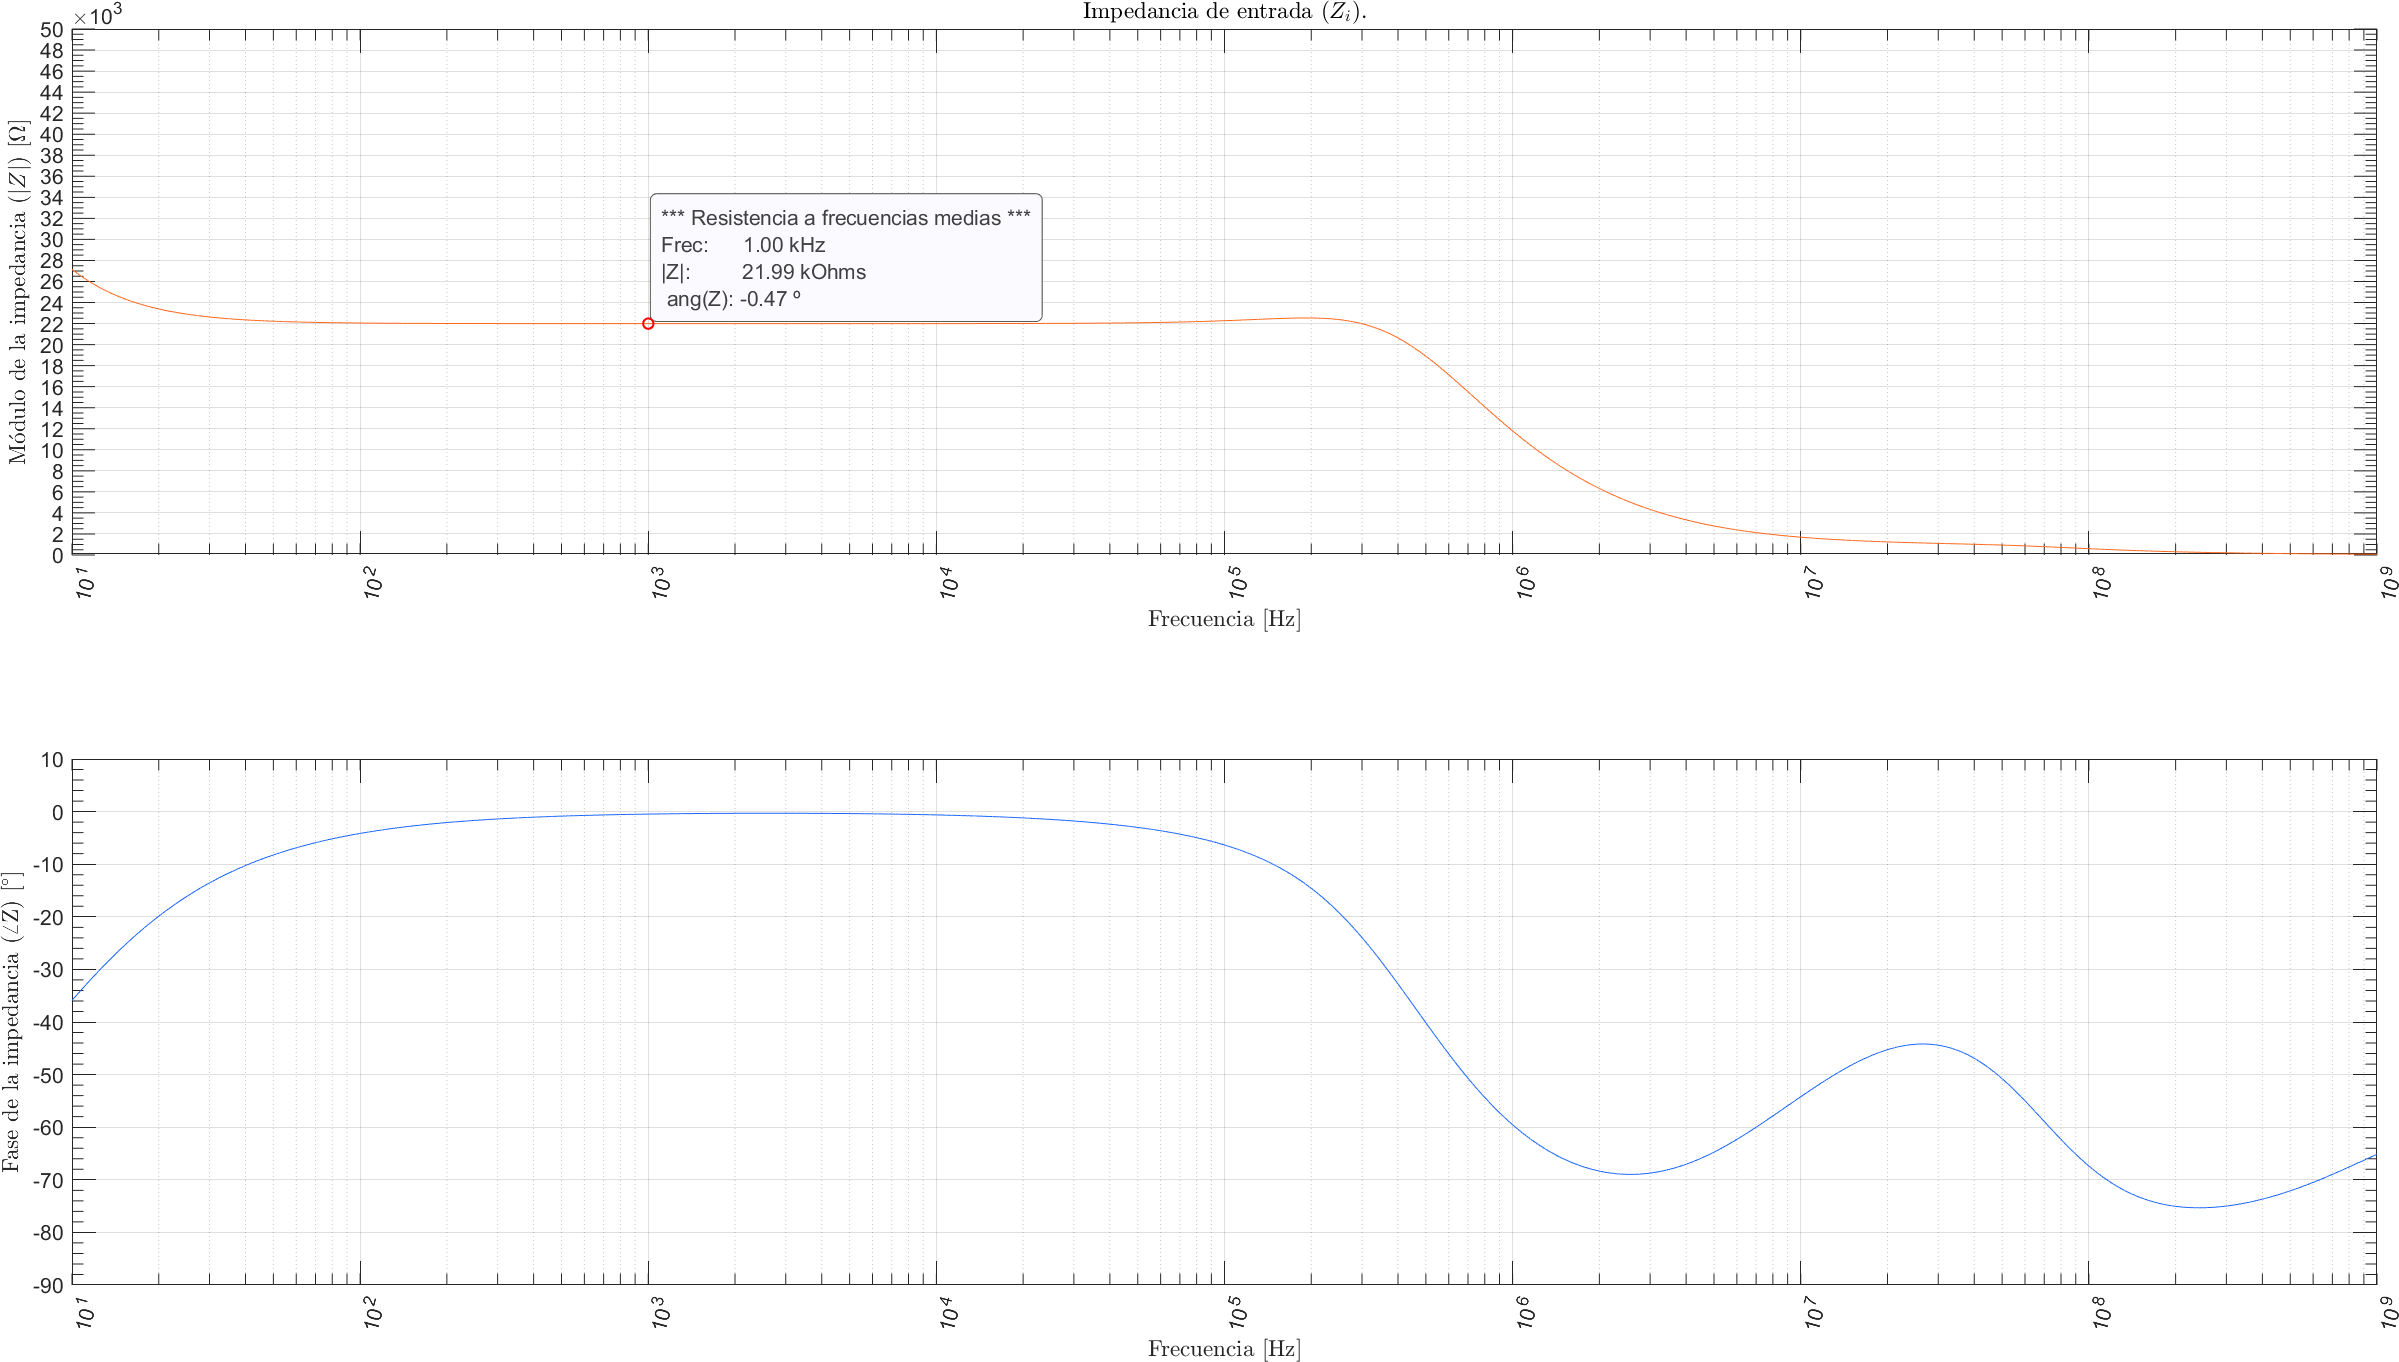
\includegraphics[height=0.66 \textwidth, angle=90]{./img/simulaciones/Impedance/amplifier_Zi.png}
    \caption{Valores de impedancia de entrada (simulación).}
    \label{fig:amplifier_Zi_sim}
\end{figure}

\clearpage

\begin{figure}[H]
    \centering
    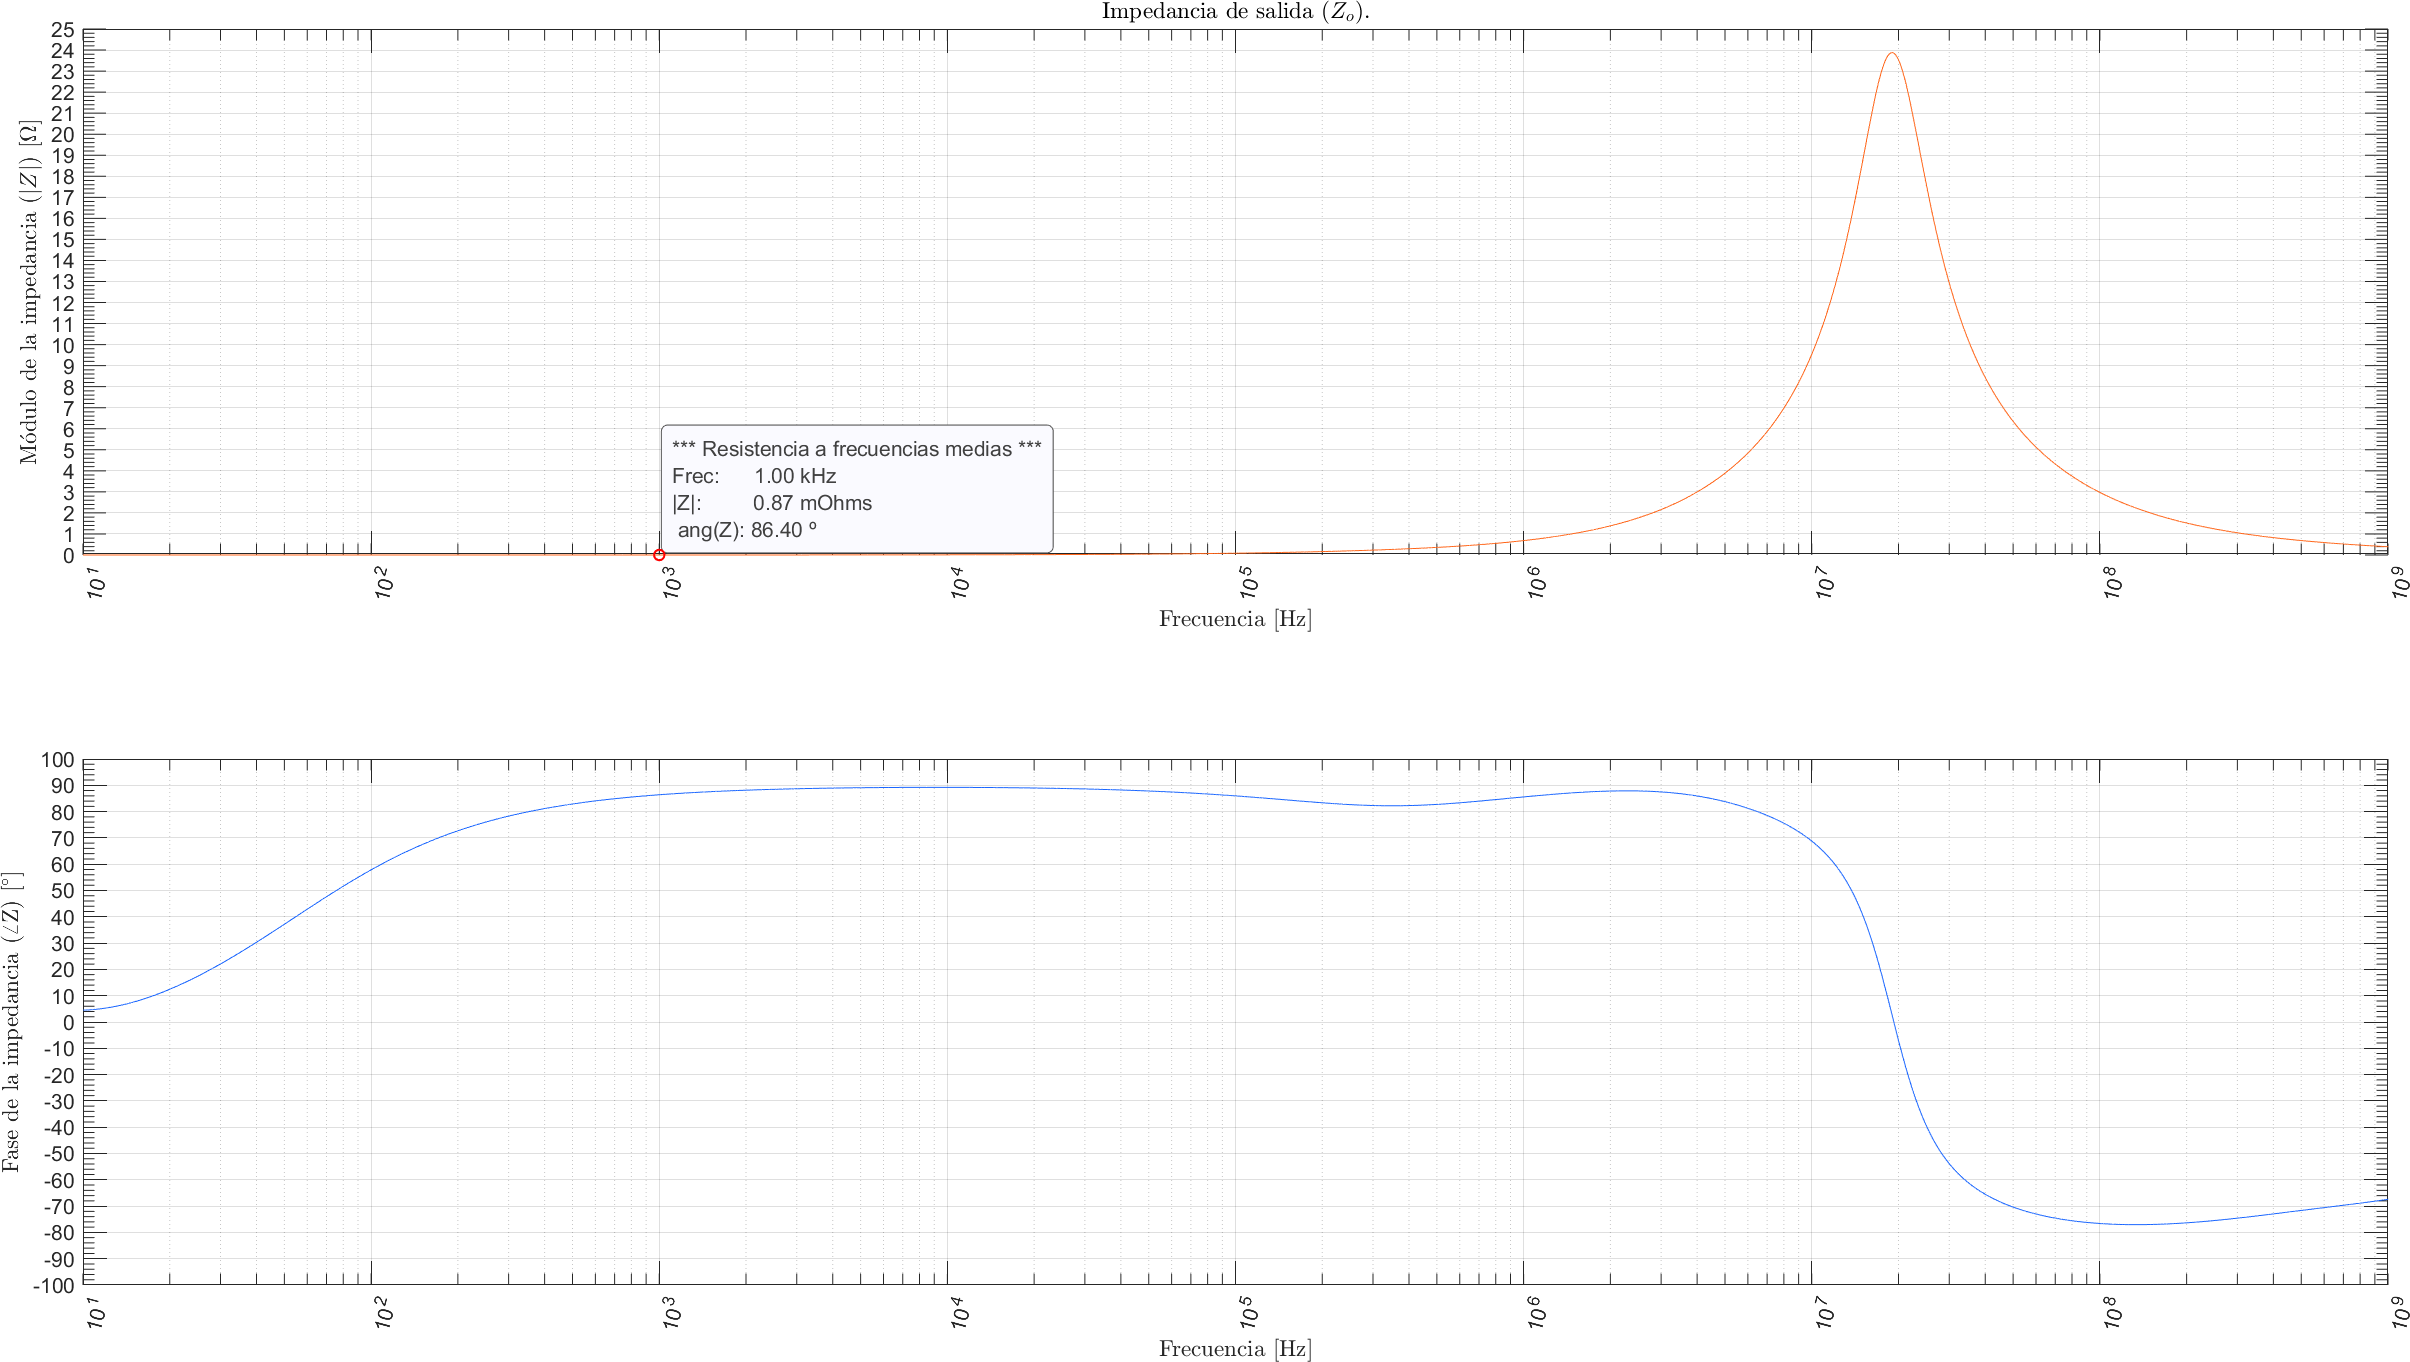
\includegraphics[height=0.66 \textwidth, angle=90]{./img/simulaciones/Impedance/amplifier_Zo.png}
    \caption{Valores de impedancia de salida (simulación).}
    \label{fig:amplifier_Zo_sim}
\end{figure}

\clearpage

\subsection{THD}

\begin{figure}[H]
    \centering
    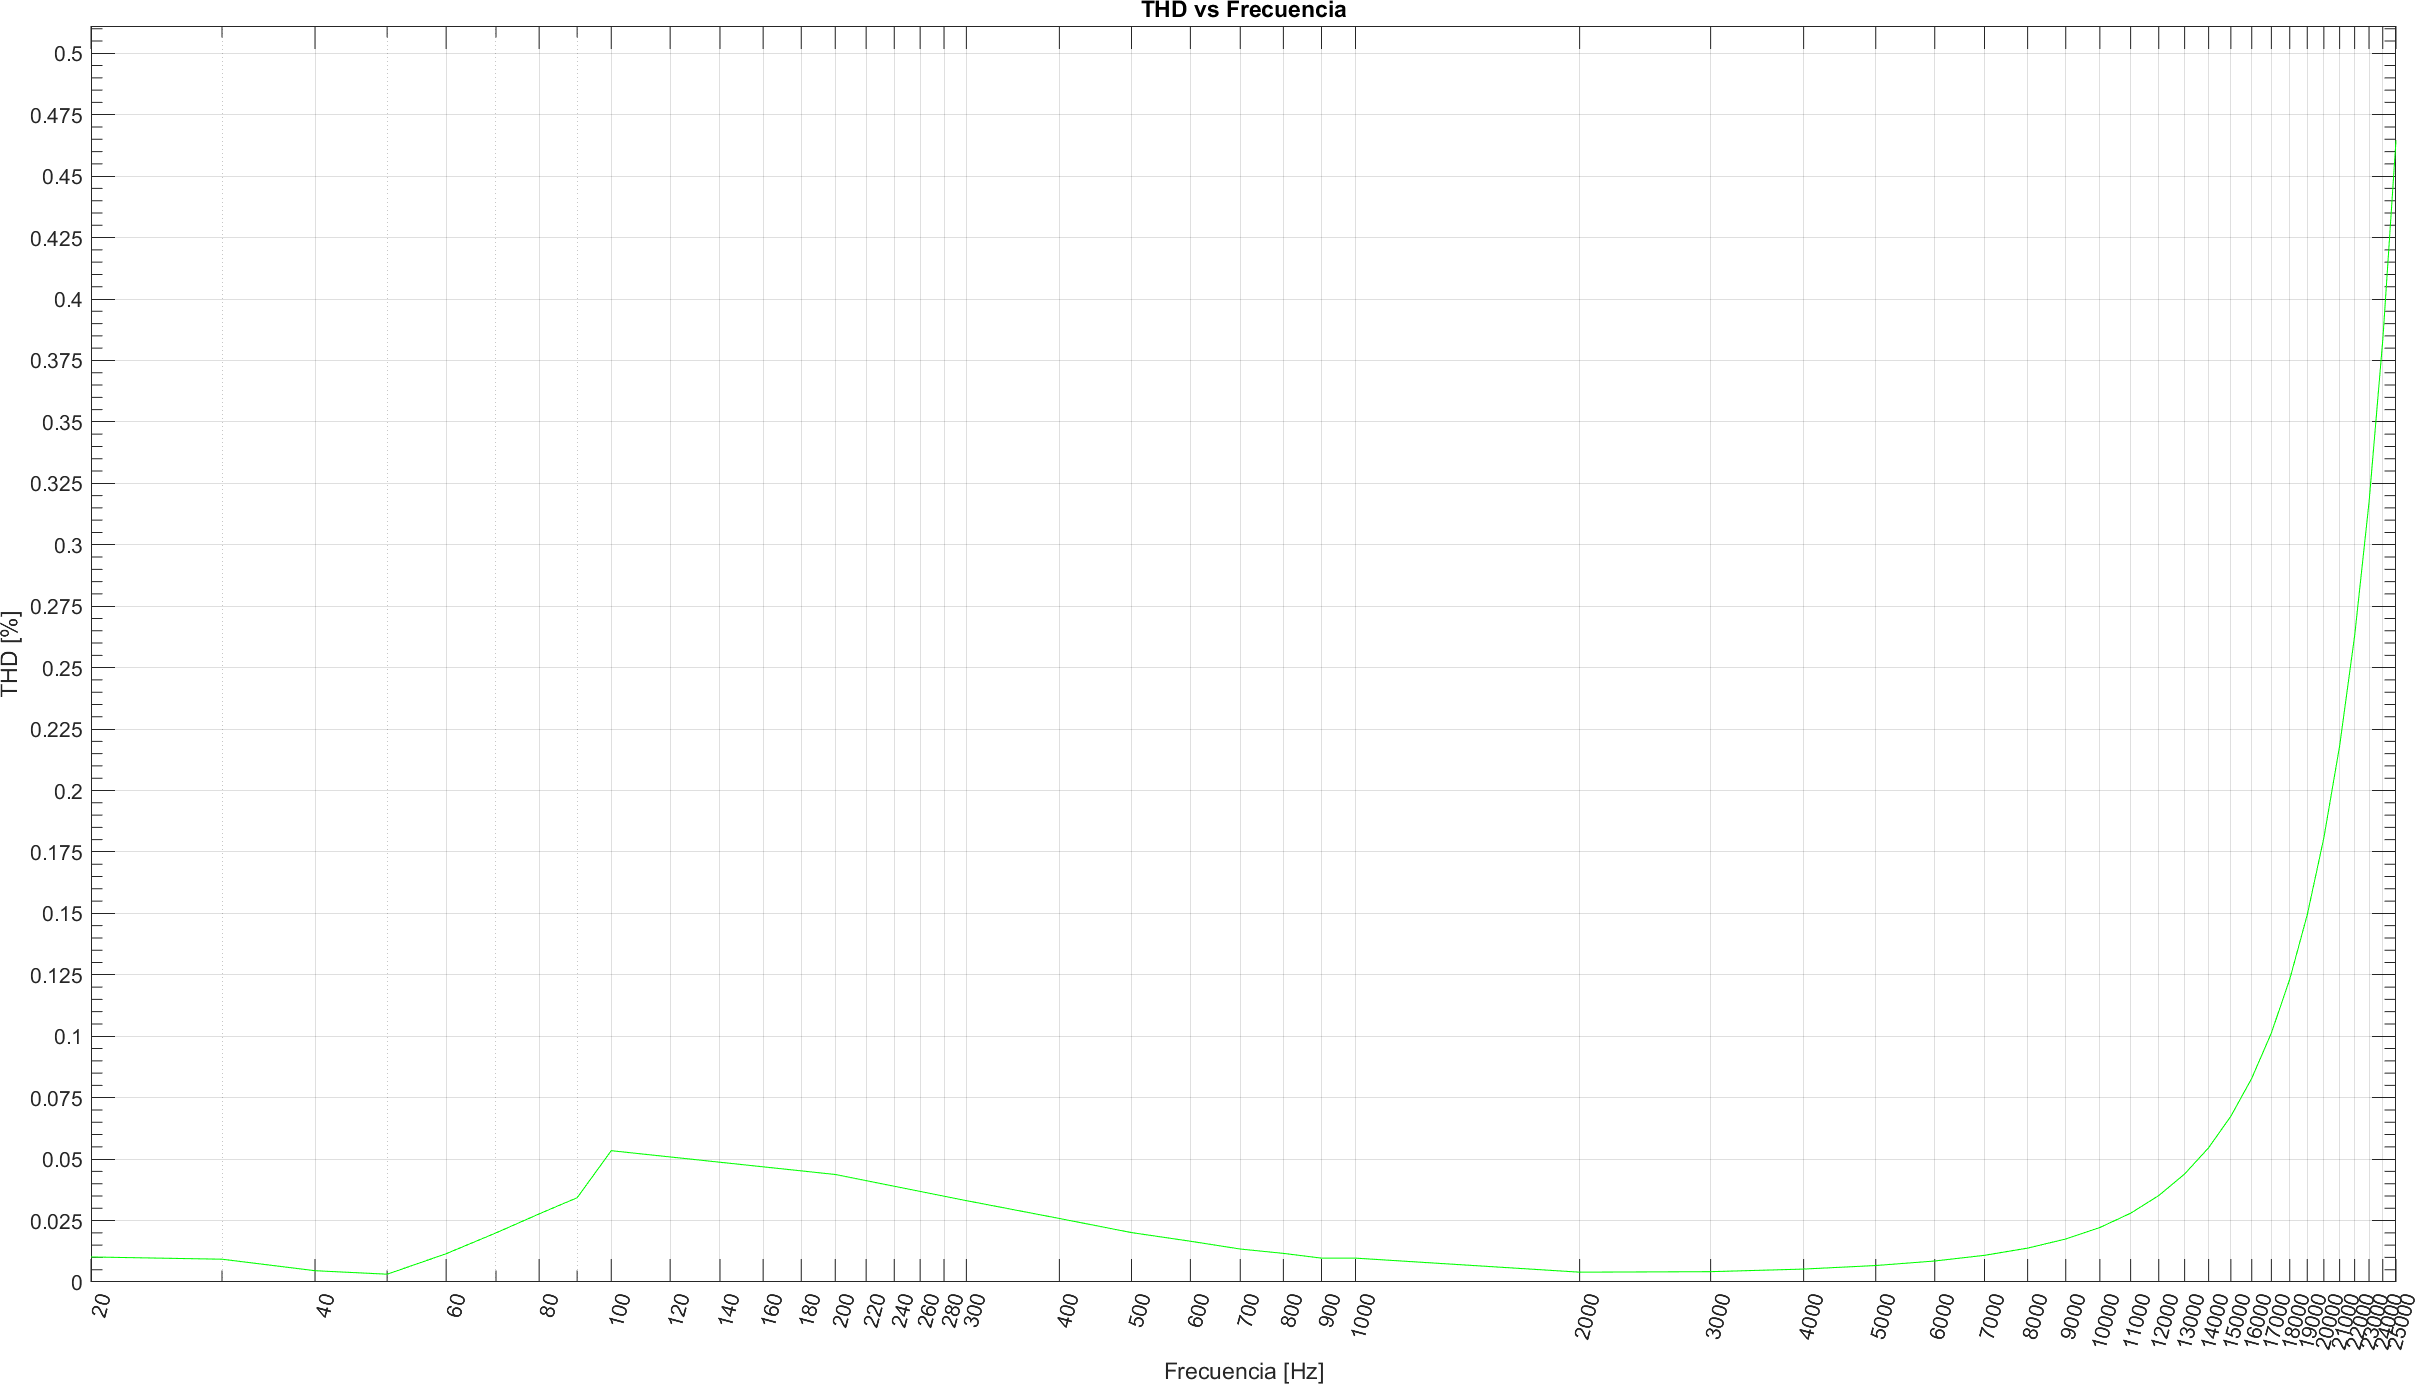
\includegraphics[height=0.66 \textwidth, angle=90]{./img/simulaciones/THD/THD_vs_frequency_sim.png}
    \caption{THD en función de la frecuencia (simulación).}
    \label{fig:THD_vs_frequency_sim}
\end{figure}

\clearpage

\begin{figure}[H]
    \centering
    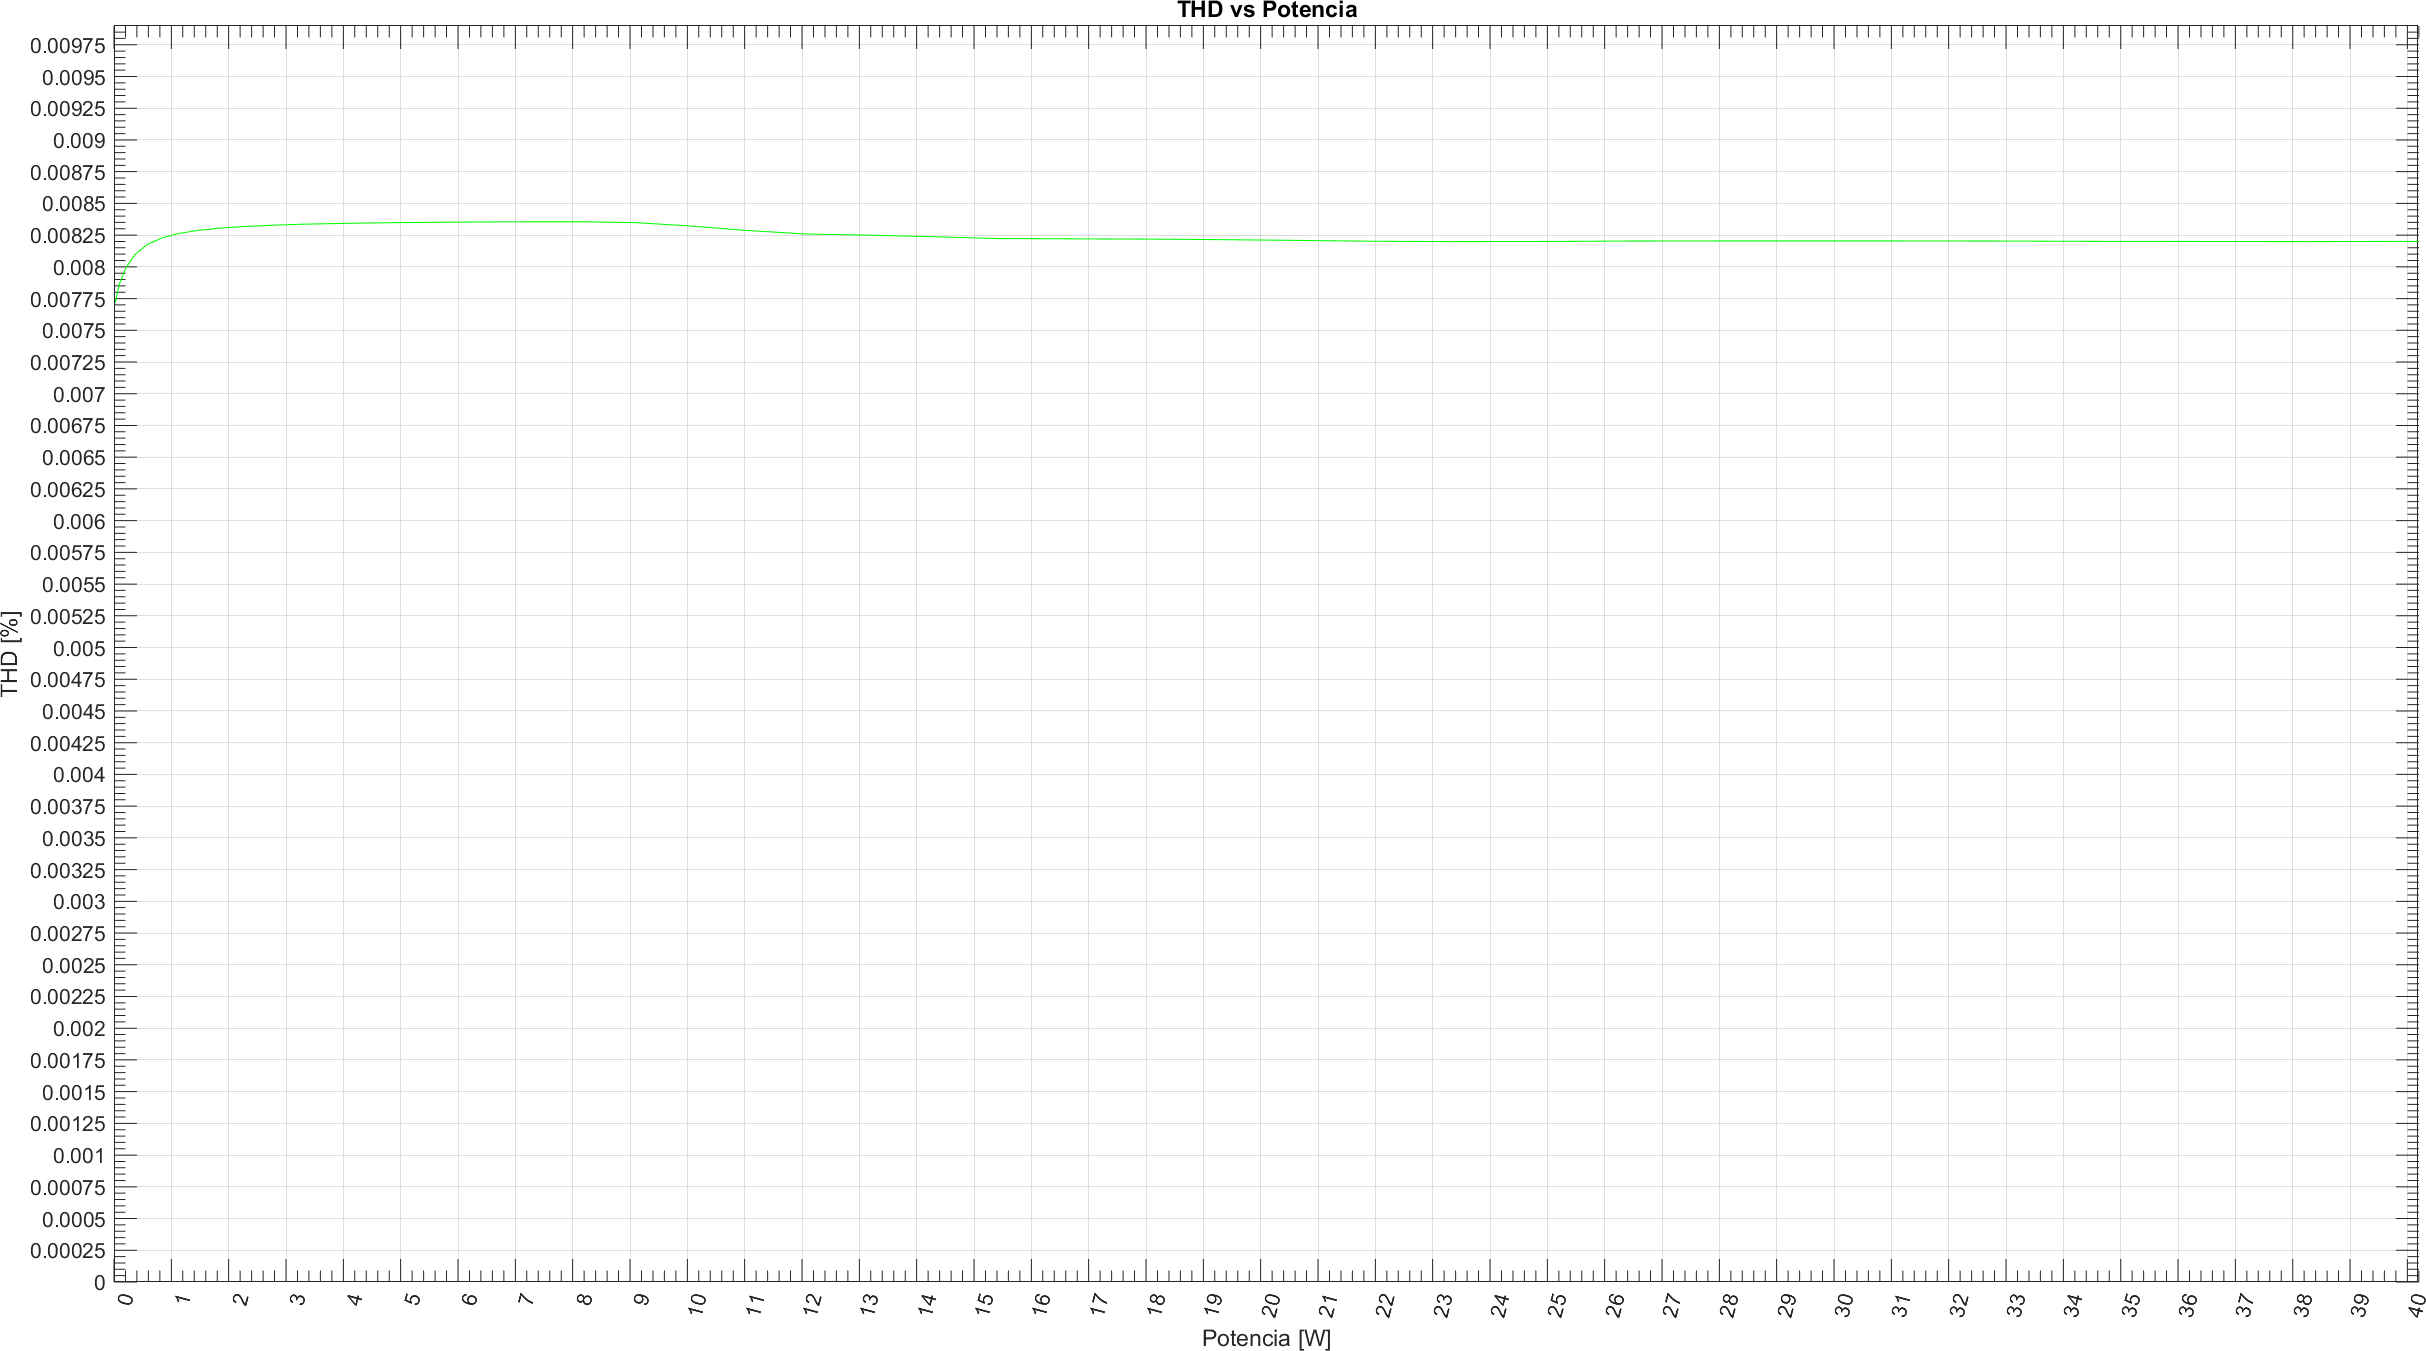
\includegraphics[height=0.66 \textwidth, angle=90]{./img/simulaciones/THD/THD_vs_power_sim.png}
    \caption{THD en función de la potencia (simulación).}
    \label{fig:THD_vs_power_sim}
\end{figure}

\clearpage

\subsection{Slew Rate}

\par En la figura ~\figref{fig:Slew_Rate} observamos el resultado de la simulación utilizada para el cálculo del Slew Rate. En la figura  ~\figref{fig:Slew_Rate_zoom}, se aprecia con más claridad la pendiente para el cálculo, además del efecto que produce la conmutación entre las fuentes de $15 \si[per-mode=symbol]{\volt}$ y $35 \si[per-mode=symbol]{\volt}$.

\par A partir del cálculo de la pendiente producida por la respuesta al escalón obtenemos como resultado del Slew Rate:

\begin{itemize}
    \item Slew Rate = $4.79 \si[per-mode=symbol]{\volt\per\micro\second}$
\end{itemize}

\vfill

\clearpage

\begin{figure}[H]
    \centering
    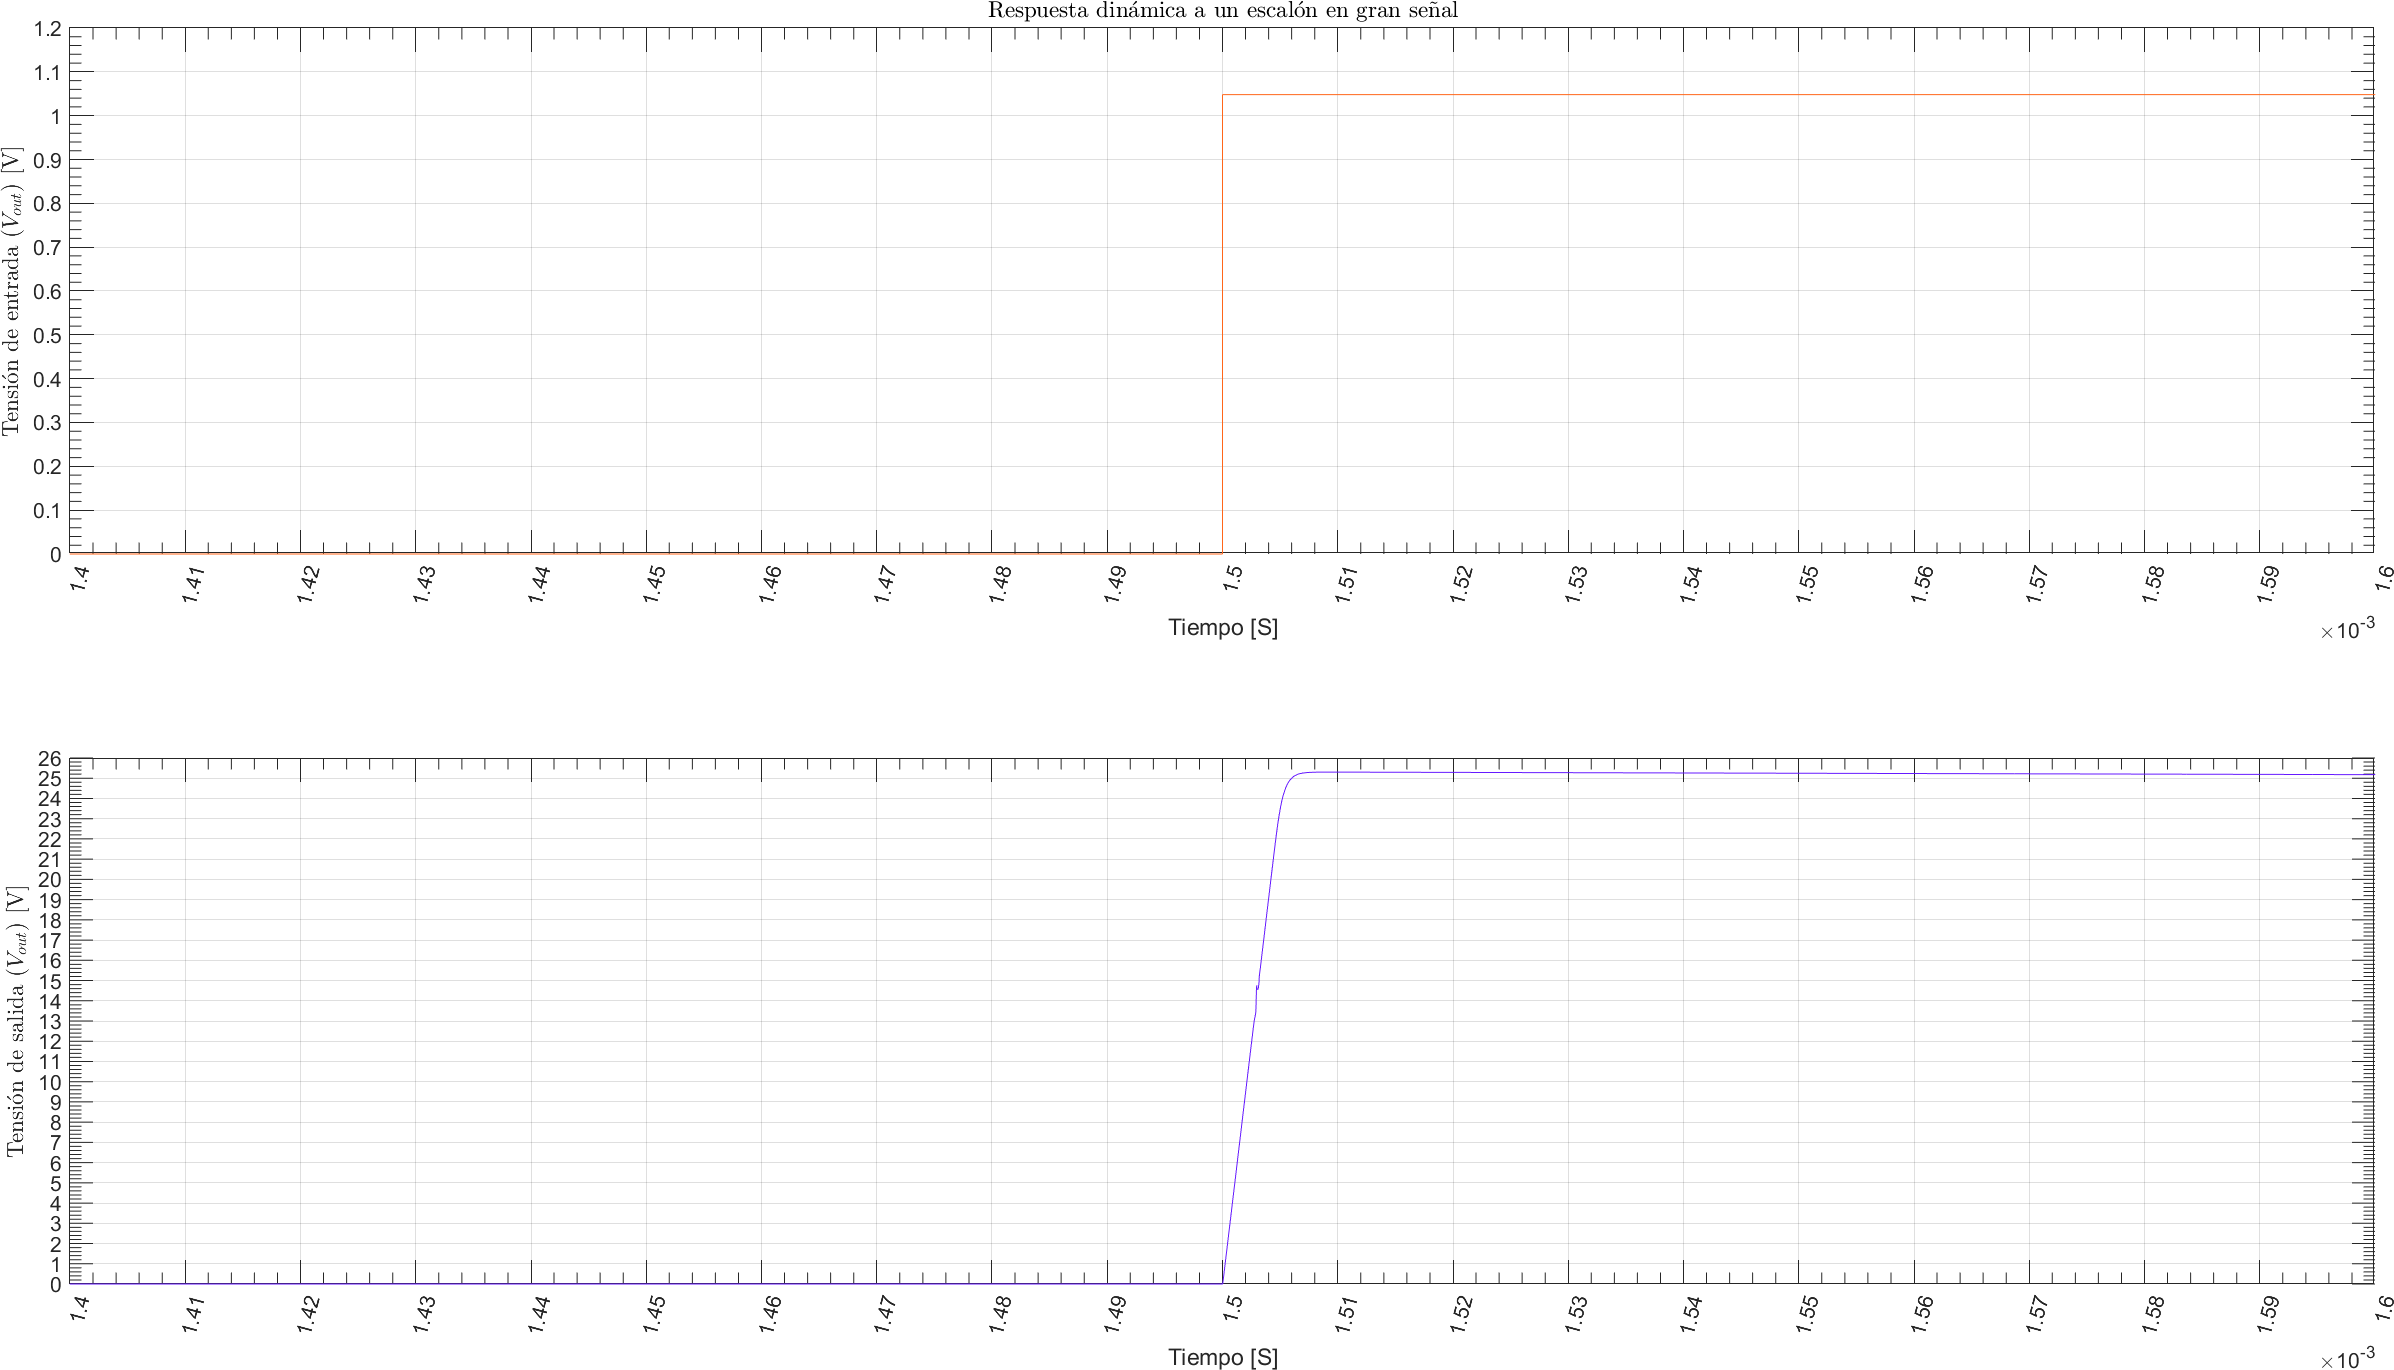
\includegraphics[height=0.66 \textwidth, angle=90]{./img/simulaciones/Slew_Rate/Slew_Rate.png}
    \caption{Tiempo de crecimiento (simulación).}
    \label{fig:Slew_Rate}
\end{figure}

\clearpage

\begin{figure}[H]
    \centering
    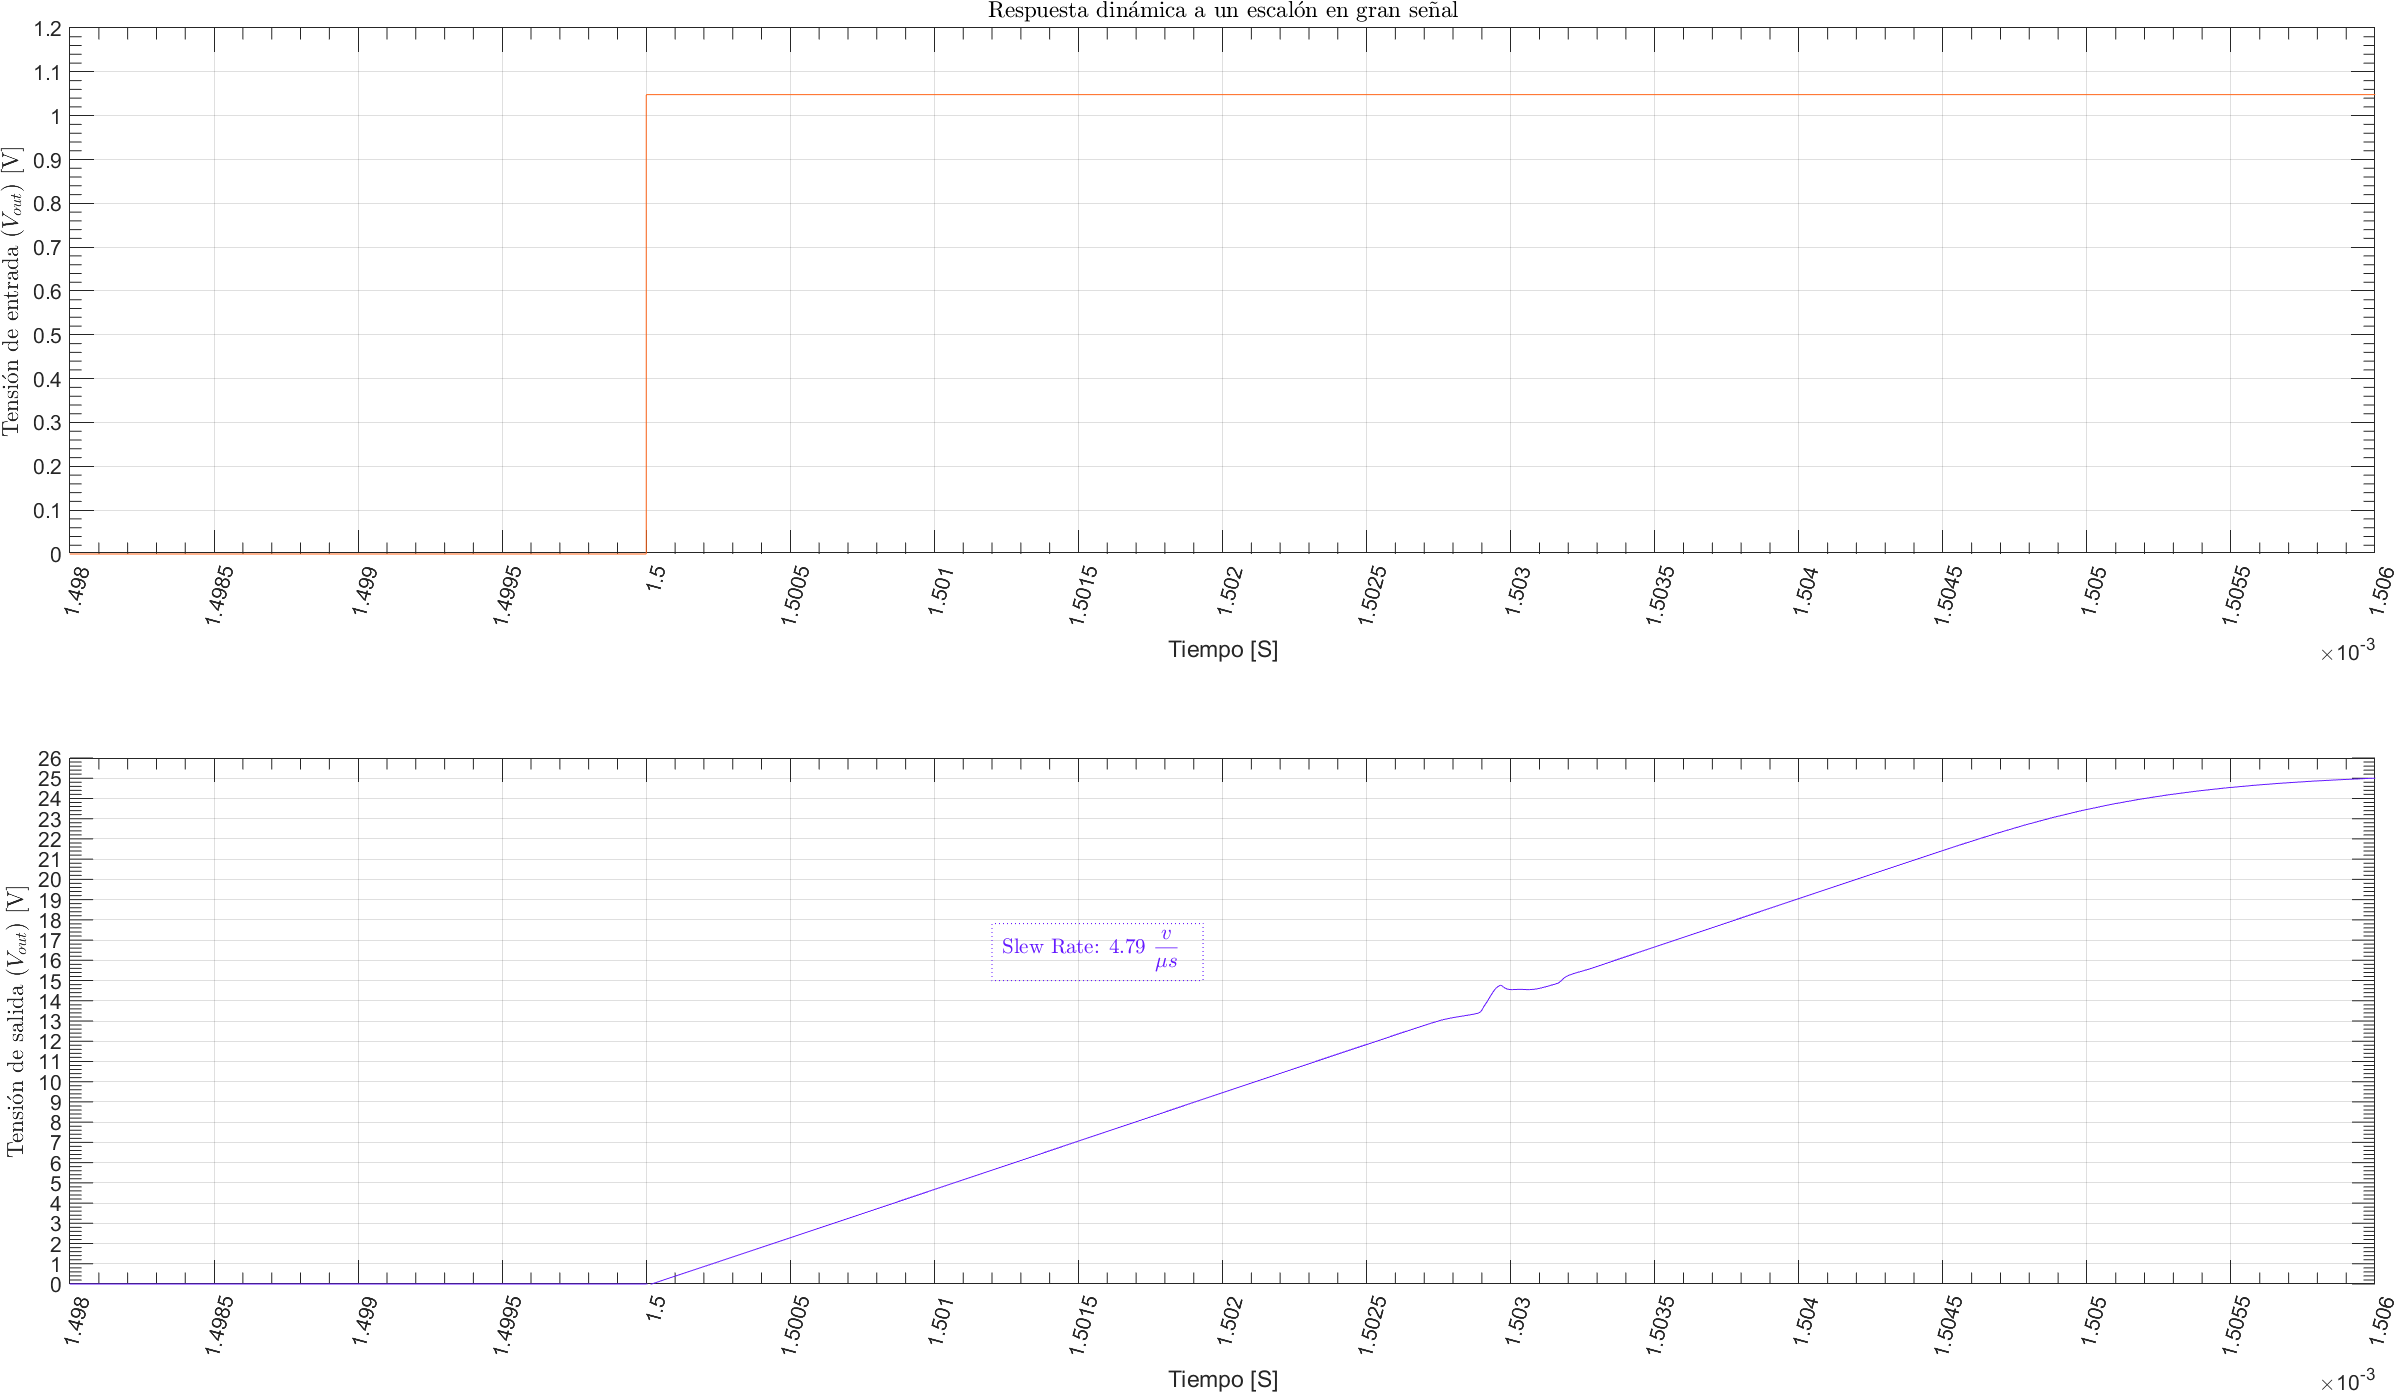
\includegraphics[height=0.66 \textwidth, angle=90]{./img/simulaciones/Slew_Rate/amplifier_SR_zoom.png}
    \caption{Tiempo de crecimiento, zoom sobre la pendiente  (simulación).}
    \label{fig:Slew_Rate_zoom}
\end{figure}

\clearpage
\clearpage
%%\\\\\\\\\\\\\\\\\\\\\\\\\\\
%
%%\\\\\\\\\\\\\\\\\\\\\\\\\\\
%\section{Alimentación}
%\resetallcounters
%


Se colocaron capacitores ($CF_{1}$ a $CF_{8}$) en los 4 rieles de alimentación ($\pm 49 \si[per-mode=symbol]{\volt}$ y $\pm 15 \si[per-mode=symbol]{\volt}$) para filtrar ripple y ruidos en los rieles de alimentación, estos filtros se colocan cerca a la etapa de salida, y luego siguiendo las recomendaciones del libro se retorna hacia el filtro que alimenta las primeras etapas, cuidando de que los retornos sean al punto de tierra sin compartir los retornos. son pares de capacitores, uno electrolítico para filtrar principalmente el ripple de la fuente y el otro cerámico para compensar efectos inductivos y filtrar ruido de alta frecuencia introducido por el switcheo de los transistores de salida.


\subsection{Diseño de la fuente de alimentación}


\label{sec:fuente}

En nuestro proyecto vamos a utilizar una fuente no regulada con protecciones, la misma está realizada con un transformador de varias salidas, $36 \si[per-mode=symbol]{\volt} + 36 \si[per-mode=symbol]{\volt}$ y $12 \si[per-mode=symbol]{\volt} + 12 \si[per-mode=symbol]{\volt}$, otra opción son dos transformadores con punto medio independientes, ambas opciones se estudiaron y están comercialmente disponibles, en el primer caso es un diseño a medida por encargo, la decisión no hace al funcionamiento y se tomará por razones económicas y de tamaño. Los secundarios se rectifican con puentes de diodos integrados y se filtran con capacitores electrolíticos de alto valor, calculados en base a lo indicado por las simulaciones. Las protecciones consisten en limitadores de corriente, son circuitos típicos armados alrededor de un transistor bipolar con una resistencia de sensado y un \textbf{MOSFET} de potencia de paso con baja $R_{ds_{on}}$, estos circuitos se repiten para los cuatro rieles con limitaciones apropiadas en cada caso, los valores a los cuales se limitan las corrientes son suficientes para ser soportados por el tiempo necesario para quemar los fusibles en serie que tiene cada riel, de esta manera se protege al circuito de la fuente de alimentación y al amplificador, el cual tiene su propia protección para los transistores de salida, pero es muy por arriba de lo que la fuente puede entregar, ambas protecciones se complementan, evitando que ningún circuito se dañe, mas allá de los fusibles.

\vfill

\clearpage


\begin{figure}[H]
	\centering
	\includegraphics[width=0.7\paperheight, angle=90]{img/power_supply.png}
	\caption{Fuente de alimentación.}
	\label{fig:power_supply}
\end{figure}
%\clearpage
%%\\\\\\\\\\\\\\\\\\\\\\\\\\\
%
%%\\\\\\\\\\\\\\\\\\\\\\\\\\\
%\section{Diseño del pre-amplificador}
%\resetallcounters
%
Como etapa de pre-procesamiento, elegimos un pre-amplificador relativamente sencillo que implementa, control de volumen, selección de sensibilidad para tres fuentes de audio, \textbf{consumer} (cualquier fuente de un equipo comercial, como ser un celular), \textbf{línea} (fuente de valor standard como ser la salida de una placa de sonido) y \textbf{guitarra}, además el circuito implementa un control básico de tonos, con control de \textbf{Bass} y \textbf{Trebel}, con lo cual se tiene una llave selectora de tres puntos, un potenciómetro logarítmico para el volumen y dos potenciómetros lineales para el control de tonos. Para la implementación se necesitan tres amplificadores operacionales, para esta función seleccionamos el operacional \textbf{NE5532} de \textbf{Texas}, por su diseño específico para audio y su bajo ruido. El circuito es simple, la primer etapa es un atenuador conectado a la entrada de un amplificador no inversor, acoplado capacitivamente, la segunda etapa es un operacional con dos redes de realimentación para atenuar o graves alrededor de $100 \si[per-mode=symbol]{\hertz}$ o agudos alrededor de $10 \si[per-mode=symbol]{\kilo\hertz}$, el circuito original amplificaba, pero para adecuarlo a la sensibilidad de nuestro amplificador lo modificamos para que siempre la salida esté por debajo de $\si[per-mode=symbol]{1.1 \volt}$, para esto el circuito cuenta con una serie de presets en la etapa de salida que permiten ajustar el selector de sensibilidades y la ganancia global para adaptarse perfectamente a nuestro amplificador.


\vfill

\clearpage


\begin{figure}[H]
	\centering
	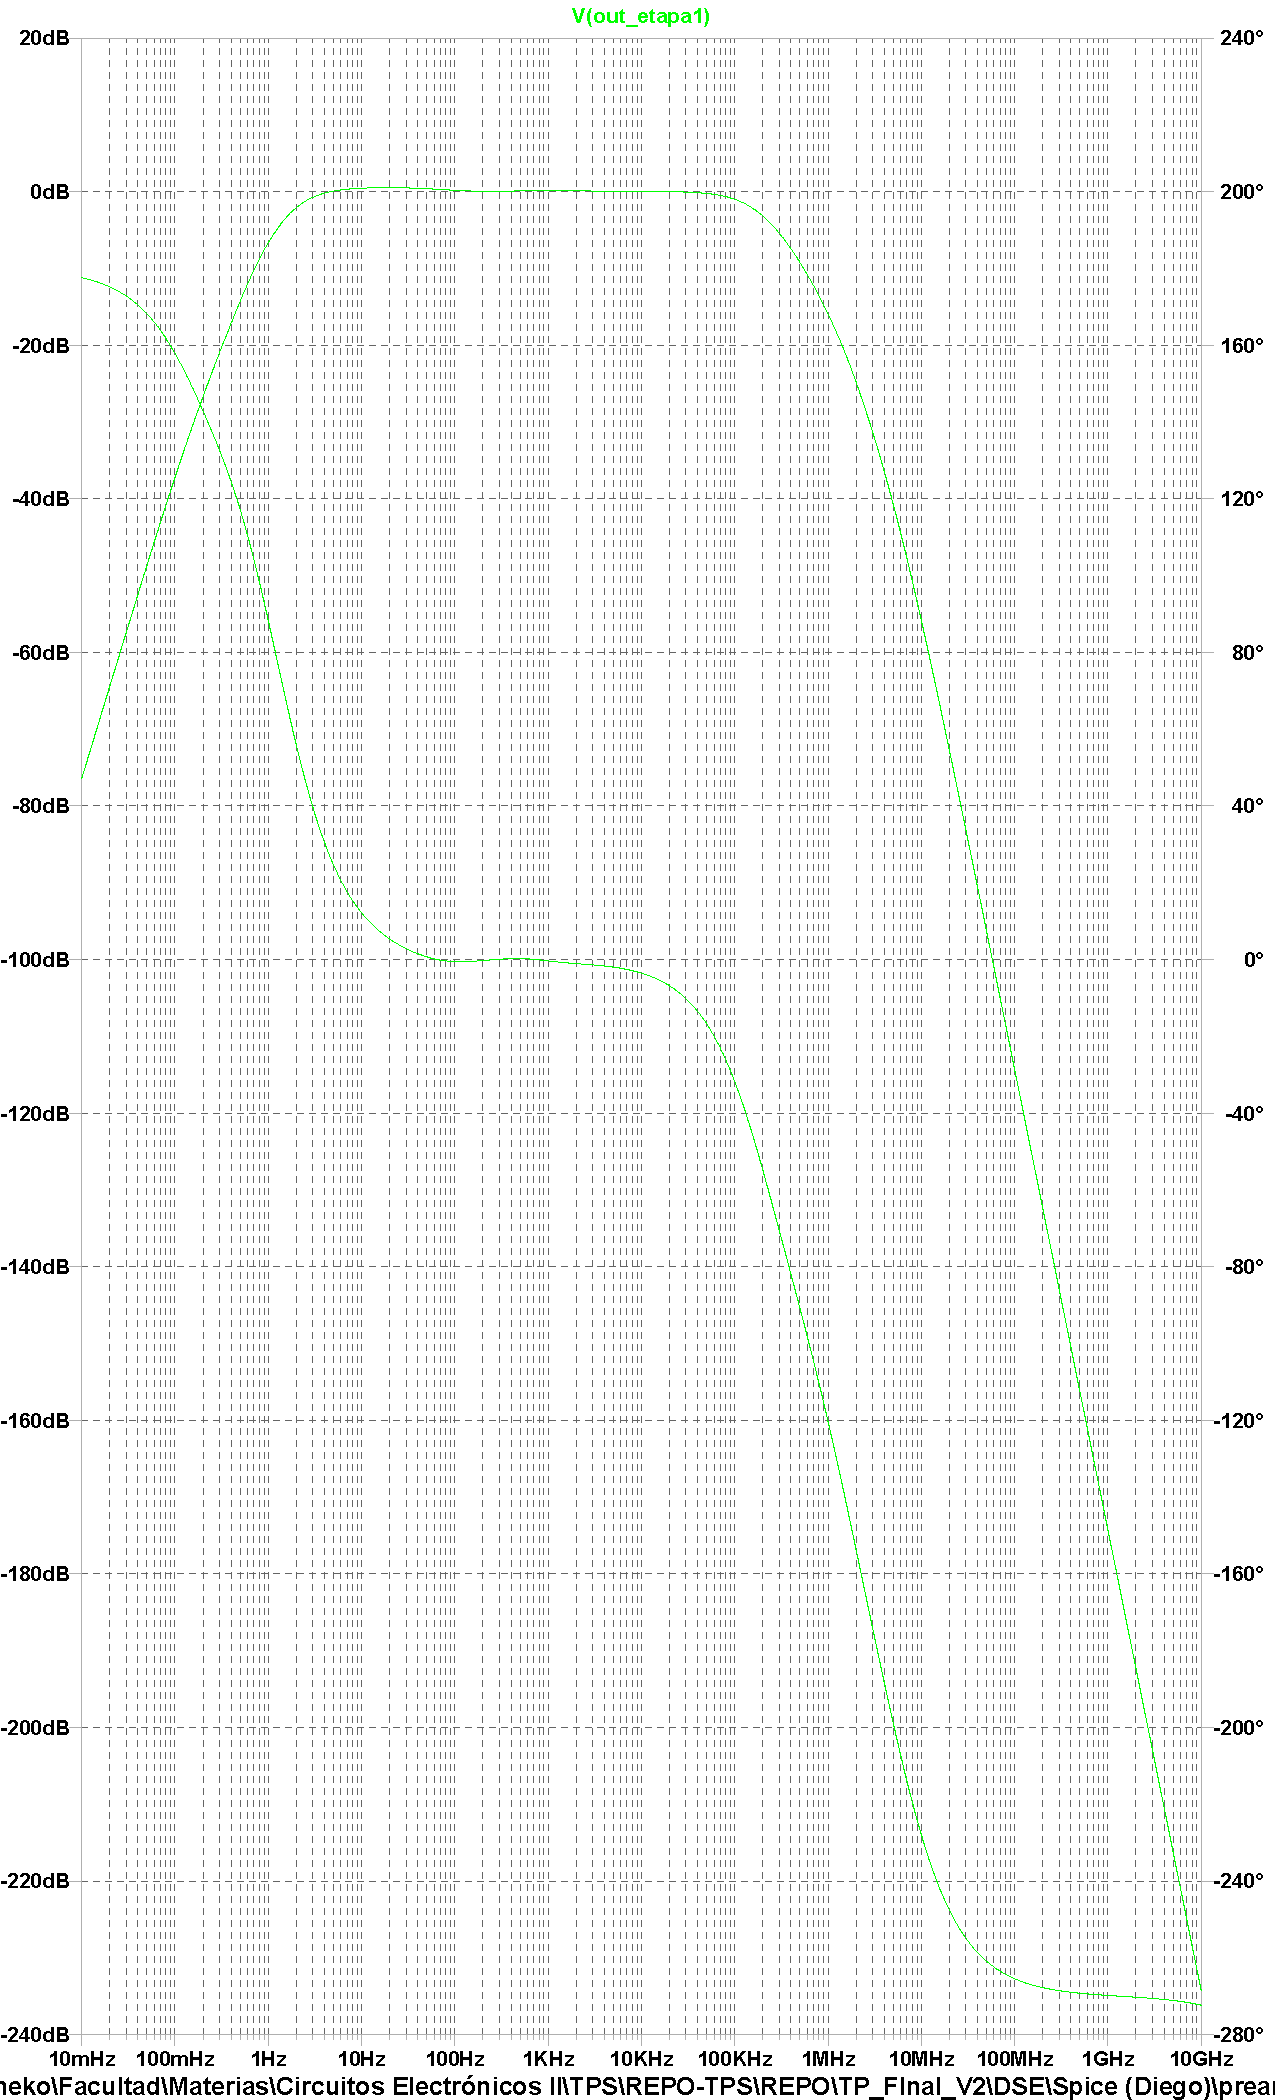
\includegraphics[width=0.7\paperheight, angle=90]{img/preamp.png}
	\caption{pre-amplificador con control de tonos y volumen.}
	\label{fig:power_supply}
\end{figure}
%\clearpage
%%\\\\\\\\\\\\\\\\\\\\\\\\\\\
%
%
%%\\\\\\\\\\\\\\\\\\\\\\\\\\\
%\section{Diseño de PCB}
%\resetallcounters
%\input{PCB}
%\clearpage
%%\\\\\\\\\\\\\\\\\\\\\\\\\\\
%
%
%%\\\\\\\\\\\\\\\\\\\\\\\\\\\
%\section{Disipación de calor}
%\resetallcounters
%\input{heat_sink}
%\clearpage
%%\\\\\\\\\\\\\\\\\\\\\\\\\\\

%%\\\\\\\\\\\\\\\\\\\\\\\\\\\
\section{Mediciones}
\resetallcounters
\subsection{Instrumental}

\label{sec:instrumentos}

Para las mediciones durante la validación del prototipo, se utilizó el instrumental provisto por la facultad en sus laboratorios. \\

Se utilizó para alimentar nuestro prototipo en todas las mediciones un par de fuentes de alimentación tipo \textit{M10SP3010E}, que es una fuente de $\pm 30 \si[per-mode=symbol]{\volt}$ como máximo, $10 \si[per-mode=symbol]{\ampere}$ de corriente máxima y limitación de corriente ajustable, la misma puede verse en la figura~\figref{fig:power_supply_lab}. La fuente mencionada fue complementada con un par de fuentes switching de $\pm 10 \si[per-mode=symbol]{\volt}$, armadas conectando de a pares $\num 4$ fuentes de $\pm 5 \si[per-mode=symbol]{\volt}$ y $4 \si[per-mode=symbol]{\ampere}$ de corriente máxima, para llegar a los $\pm 35 \si[per-mode=symbol]{\volt}$ requeridos por nuestro prototipo.


\begin{figure}[H]
    \centering
    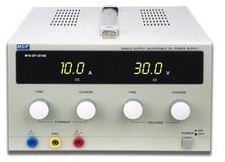
\includegraphics[width=0.5 \textwidth]{./img/instrumentos/M10SP3010E.png}
    \caption{Fuente de alimentación \textit{M10SP3010E}.}
    \label{fig:power_supply_lab}
\end{figure}



Para todas las mediciones realizadas sobre el circuito se utilizó ya sea un osciloscopio, un multímetro, o ambos, los instrumentos utilizados fueron un multímetro \textit{true-rms} tipo \textit{MT-1707}, el mismo puede ver en la figura~\figref{fig:multimeter_lab}. El mismo se pidió específicamente por ser \textit{true-rms}, lo que permite hacer mediciones precisas de avlores eficaces para cualquier tipo de onda, hasta los $3 \si[per-mode=symbol]{\kilo\hertz}$ aproximadamente. El osciloscopio utilizado es del tipo \textit{ATTEN ADS1102CAL}, el cual puede verse en la figura~\figref{fig:osciloscope_lab}, el mismo se eligió de entre los disponibles, por poseer la posibilidad de realizar capturas de lo medido hacia un pendrive.


\begin{figure}[H]
    \centering
    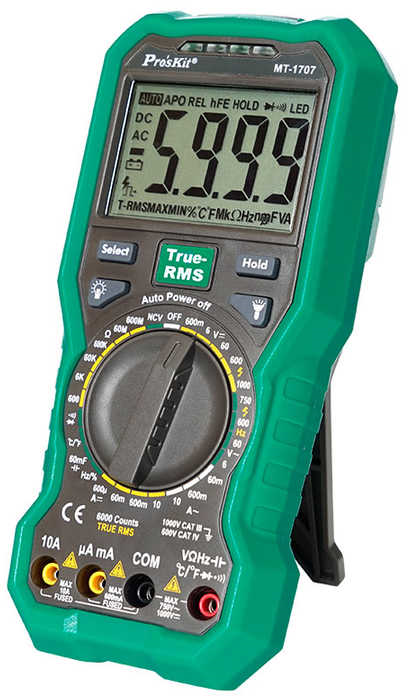
\includegraphics[width=0.5 \textwidth]{./img/instrumentos/MT_1707.png}
    \caption{Multímetro \textit{MT-1707}.}
    \label{fig:multimeter_lab}
\end{figure}


\begin{figure}[H]
    \centering
    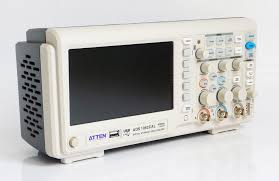
\includegraphics[width=0.5 \textwidth]{./img/instrumentos/ATTEN_ADS1102CAL.png}
    \caption{Osciloscopio \textit{ATTEN ADS1102CAL}.}
    \label{fig:osciloscope_lab}
\end{figure}


Para excitar al prototipo se usaron generadores de señal, en casi todas las mediciones se usó un generador del tipo \textit{FG-8002}, el mismo usa conformación de onda para la generación de señales senoidales, el mismo se puede ver en la figura~\figref{fig:signalgen1_lab}, el hecho de que use conformación de onda para la generación de señales senoidales, hace que las misma tengan un contenido armónico que lo hace inadecuado para el caso de la medición de distorsión armónica, para eso se utilizó un generador tipo \textit{GWINSTEK GAG-810}, el mismo puede verse en la figura~\figref{fig:signalgen2_lab}, este es un generador basado en osciladores senoidales, lo cual permite que tenga bajo contenido armónico.


\begin{figure}[H]
    \centering
    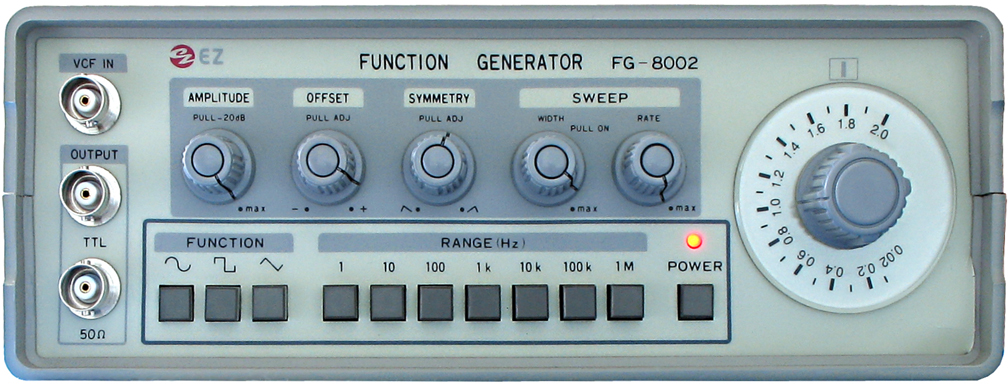
\includegraphics[width=0.5 \textwidth]{./img/instrumentos/FG_8002.png}
    \caption{Generados de señales \textit{FG-8002}.}
    \label{fig:signalgen1_lab}
\end{figure}

\vfill

\clearpage


\begin{figure}[H]
    \centering
    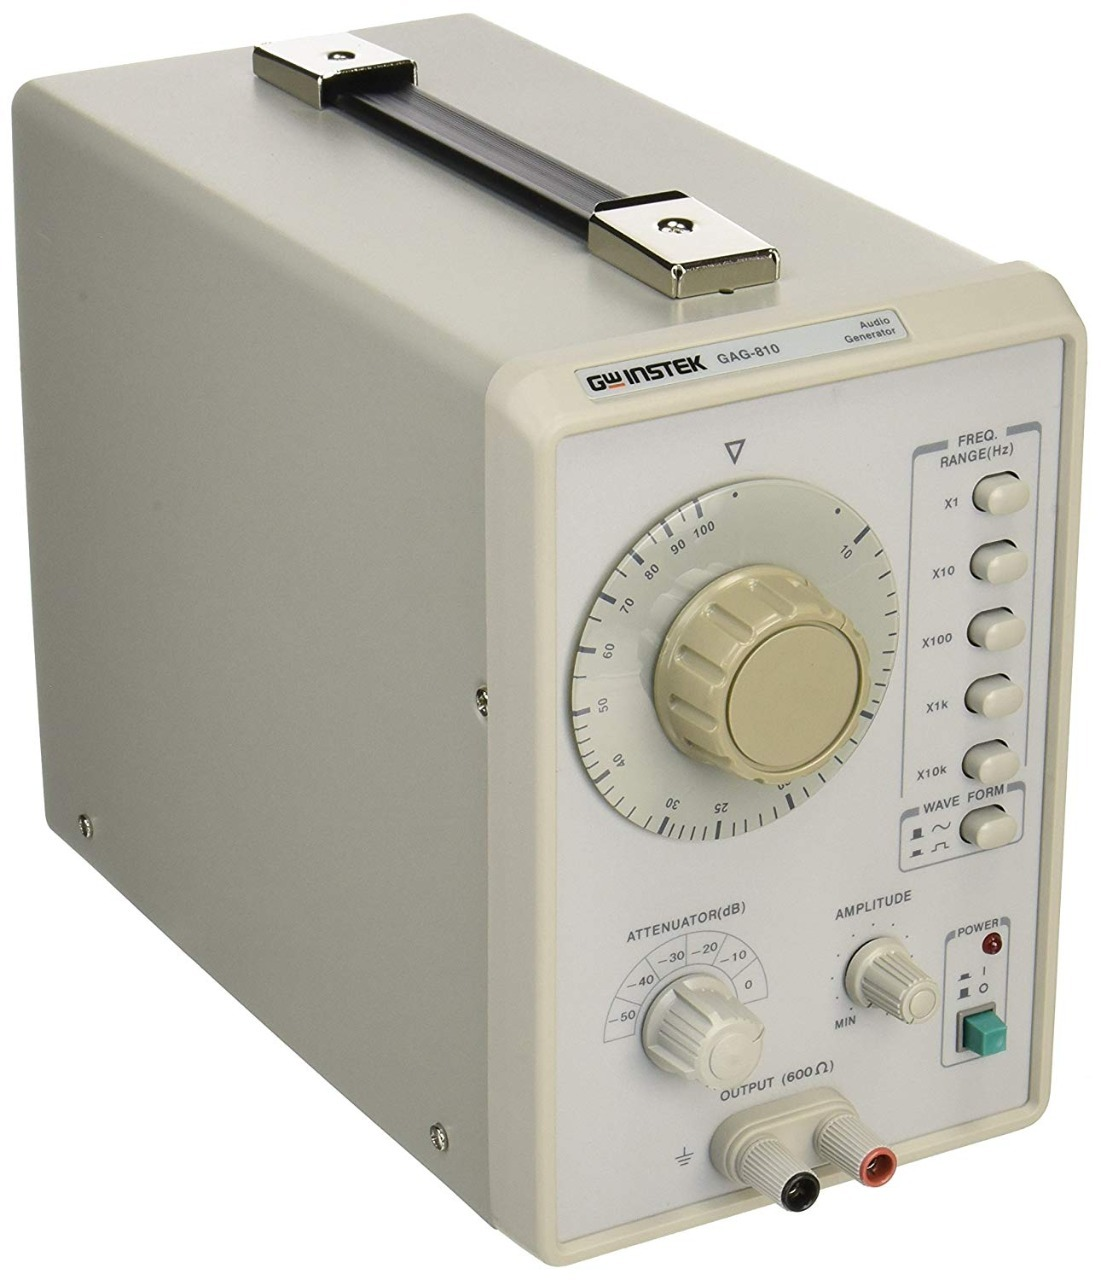
\includegraphics[width=0.5 \textwidth]{./img/instrumentos/GWINSTEK_GAG_810.png}
    \caption{Generados de señales \textit{GWINSTEK GAG-810}.}
    \label{fig:signalgen2_lab}
\end{figure}



Finalmente durante el armado y testeo de la fuente switching que se diseño para proveer las tensiones de $\pm 15 \si[per-mode=symbol]{\volt}$, se utilizó un \textit{LCR} tipo \textit{PROTOMAX VA511} para medir los inductores utilizados, el mismo puede verse en la figura~\figref{fig:lcr_lab}

\vfill

\clearpage


\begin{figure}[H]
    \centering
    \includegraphics[width=0.5 \textwidth]{./img/instrumentos/LCR_PROTOMAX_VA511.png}
    \caption{LCR \textit{PROTOMAX VA511}.}
    \label{fig:lcr_lab}
\end{figure}

\clearpage


\subsection{Mediciones}



\subsubsection{Polarización}


Para las mediciones de la polarización se utilizó solo el multímetro digital antes mencionado, figura~\figref{fig:multimeter_lab}, no fue necesario otro instrumental para esta parte, las corrientes se midieron usando las caídas en resistores y abriendo el circuito cuando ello era posible.\\

Se realizaron las mediciones de punto de polarización del amplificador sin señal aplicada, obteniéndose los resultados del cuadro~\tableref{tab:PuntoQ1}. Los mismos se verificaron con y sin la carga conectada para observar que no haya cambios en la polarización, una vez ajustada la corriente de polarización de salida, para este primer caso se ajustó la corriente de los transistores de salida en aproximadamente $190 \si[per-mode=symbol]{\milli\ampere}$. El segundo caso medido se muestra en el cuadro~\tableref{tab:PuntoQ2}, en este caso se ajusto la corriente al máximo que permite el preset del multiplicador de $V_{BE}$, aproximadamente $700 \si[per-mode=symbol]{\milli\ampere}$, como puede observarse en este caso la potencia disipada en reposo es considerable, unos $22 \si[per-mode=symbol]{\watt}$, pero puede verse como las primeras etapas prácticamente no se ven afectadas por el cambio en la corriente de reposo de los transistores de salida.


\vfill

\clearpage


\begin{table}[H]  %%\centering
    
    \setlength\arrayrulewidth{1.5pt}
    \arrayrulecolor{white}
    \def\clinecolor{\hhline{|>{\arrayrulecolor{white}}-%
    >{\arrayrulecolor{white}}|-|-|-|-|-|}}
    
\begin{center}  
\resizebox{0.7 \textwidth}{!}{%    
\begin{tabularx}{1 \textwidth}%
    {|
    >{\columncolor{white} \centering\arraybackslash}m{0.3333\linewidth}
     |
    >{\columncolor{white} \centering\arraybackslash}m{0.1667\linewidth}
     |
    >{\columncolor{white} \centering\arraybackslash}m{0.1667\linewidth}
     |
    >{\columncolor{white} \centering\arraybackslash}m{0.1667\linewidth}
     |
    >{\columncolor{white} \centering\arraybackslash}m{0.1667\linewidth}
     |
    }
    \rowcolor{HeadersColor} \thead{Transistor} & \thead{$V_{CE_{Q}}$} & \thead{$I_{C_{Q}}$} & \thead{ $P_{Q}$}\\    
    \hhline{|-|-|-|-|-|}
    %\rowcolor{Butter!20} \cellcolor{Butter!40} $I_{C}$ [$\si[per-mode=symbol]{\milli\ampere}$] & $0.54$ & $8.66$ & $9$ & $6$ & $5.5$ & $10$ & $10$  \\
    % \hhline{|-|-|-|-|-|}
    \rowcolor{gray!20} \cellcolor{gray!40} $Q_{1}$ (BC546C) & $33.87 \si[per-mode=symbol]{\volt}$  & $548.76 \si[per-mode=symbol]{\micro\ampere}$ & $ 18.57\si[per-mode=symbol]{\milli\watt}$ \\
    \hhline{|-|-|-|-|-|}
    \rowcolor{gray!20} \cellcolor{gray!40} $Q_{2}$ (BC556B) & $1.31 \si[per-mode=symbol]{\volt}$  & $548.76 \si[per-mode=symbol]{\milli\ampere}$ & $ 718.88\si[per-mode=symbol]{\micro\watt}$ \\
    \hhline{|-|-|-|-|-|}
    \rowcolor{gray!20} \cellcolor{gray!40} $Q_{3}$ (BC546B) & $31.78 \si[per-mode=symbol]{\volt}$  & $1.1 \si[per-mode=symbol]{\milli\ampere}$ & $ 34.96\si[per-mode=symbol]{\milli\watt}$ \\
    \hhline{|-|-|-|-|-|}
    \rowcolor{gray!20} \cellcolor{gray!40} $Q_{4}$ (BC556B) & $610.56 \si[per-mode=symbol]{\milli\volt}$  & $548.56 \si[per-mode=symbol]{\micro\ampere}$ & $ 334.93\si[per-mode=symbol]{\micro\watt}$ \\
    \hhline{|-|-|-|-|-|}
    \rowcolor{gray!20} \cellcolor{gray!40} $Q_{5}$ (BC546B) & $ 34.58 \si[per-mode=symbol]{\volt}$  & $548.56 \si[per-mode=symbol]{\micro\ampere}$ & $ 18.97\si[per-mode=symbol]{\milli\watt}$ \\
    \hhline{|-|-|-|-|-|}
    \rowcolor{gray!20} \cellcolor{gray!40} $Q_{6}$ (BC546B) & $29.02 \si[per-mode=symbol]{\volt}$  & $9.71 \si[per-mode=symbol]{\milli\ampere}$ & $ 281.78 \si[per-mode=symbol]{\milli\watt}$ \\
    \hhline{|-|-|-|-|-|}
    \rowcolor{gray!20} \cellcolor{gray!40} $Q_{7}$ (BC556B) & $30.32 \si[per-mode=symbol]{\volt}$  & $169.17 \si[per-mode=symbol]{\micro\ampere}$ & $ 5.13\si[per-mode=symbol]{\milli\watt}$ \\
    \hhline{|-|-|-|-|-|}
    \rowcolor{gray!20} \cellcolor{gray!40} $Q_{8}$ (BC556B) & $30.86 \si[per-mode=symbol]{\volt}$  & $9.55 \si[per-mode=symbol]{\milli\ampere}$ & $ 295.55\si[per-mode=symbol]{\milli\watt}$ \\
    \hhline{|-|-|-|-|-|}
    \rowcolor{gray!20} \cellcolor{gray!40} $Q_{9}$ (BD135) & $2.71 \si[per-mode=symbol]{\volt}$  & $9.46 \si[per-mode=symbol]{\milli\ampere}$ & $ 25.64\si[per-mode=symbol]{\milli\watt}$ \\
    \hhline{|-|-|-|-|-|}
    \rowcolor{gray!20} \cellcolor{gray!40} $Q_{10}$(BD136) & $14.09 \si[per-mode=symbol]{\volt}$  & $8.28 \si[per-mode=symbol]{\milli\ampere}$ & $ 116.67\si[per-mode=symbol]{\milli\watt}$ \\
    \hhline{|-|-|-|-|-|}
    \rowcolor{gray!20} \cellcolor{gray!40} $Q_{11}$(BD136) & $20.26 \si[per-mode=symbol]{\volt}$  & $0 \si[per-mode=symbol]{\milli\ampere}$ & $ 0\si[per-mode=symbol]{\milli\watt}$ \\
    \hhline{|-|-|-|-|-|}
    \rowcolor{gray!20} \cellcolor{gray!40} $Q_{12}$(BD135) & $20.27 \si[per-mode=symbol]{\volt}$  & $0 \si[per-mode=symbol]{\milli\ampere}$ & $ 0\si[per-mode=symbol]{\milli\watt}$ \\
    \hhline{|-|-|-|-|-|}
    \rowcolor{gray!20} \cellcolor{gray!40} $Q_{13}$(BD135) & $14.06 \si[per-mode=symbol]{\volt}$  & $9.7 \si[per-mode=symbol]{\milli\ampere}$ & $ 136.38 \si[per-mode=symbol]{\milli\watt}$ \\
    \hhline{|-|-|-|-|-|}
    \rowcolor{gray!20} \cellcolor{gray!40} $Q_{14}$(MJL21194) & $20.27 \si[per-mode=symbol]{\volt}$  & $0 \si[per-mode=symbol]{\milli\ampere}$ & $ 0\si[per-mode=symbol]{\milli\watt}$ \\
    \hhline{|-|-|-|-|-|}
    \rowcolor{gray!20} \cellcolor{gray!40} $Q_{15}$(MJL21194) & $14.72 \si[per-mode=symbol]{\volt}$  & $192.02 \si[per-mode=symbol]{\milli\ampere}$ & $ 2.83 \si[per-mode=symbol]{\watt}$ \\
    \hhline{|-|-|-|-|-|}
    \rowcolor{gray!20} \cellcolor{gray!40} $Q_{16}$(MJL21193) & $14.71 \si[per-mode=symbol]{\volt}$  & $193.5 \si[per-mode=symbol]{\milli\ampere}$ & $ 2.85 \si[per-mode=symbol]{\watt}$ \\
    \hhline{|-|-|-|-|-|}
    \rowcolor{gray!20} \cellcolor{gray!40} $Q_{17}$(MJL21193) & $20.26 \si[per-mode=symbol]{\volt}$  & $0 \si[per-mode=symbol]{\milli\ampere}$ & $ 0\si[per-mode=symbol]{\milli\watt}$ \\
    \hhline{|-|-|-|-|-|}
    \rowcolor{gray!20} \cellcolor{gray!40} $Q_{18}$(2N3906) & $1.36 \si[per-mode=symbol]{\volt}$  & $0 \si[per-mode=symbol]{\milli\ampere}$ & $ 0\si[per-mode=symbol]{\milli\watt}$ \\
    \hhline{|-|-|-|-|-|}
    \rowcolor{gray!20} \cellcolor{gray!40} $Q_{19}$(2N3904) &$1.35 \si[per-mode=symbol]{\volt}$  & $0 \si[per-mode=symbol]{\milli\ampere}$ & $ 0\si[per-mode=symbol]{\milli\watt}$ \\
    \hhline{|-|-|-|-|-|}            
    \end{tabularx}}
	\caption{Primer punto de operación.}
    \label{tab:PuntoQ1}
	\end{center}
\end{table}


\begin{table}[H]  %%\centering
    
    \setlength\arrayrulewidth{1.5pt}
    \arrayrulecolor{white}
    \def\clinecolor{\hhline{|>{\arrayrulecolor{white}}-%
    >{\arrayrulecolor{white}}|-|-|-|-|-|}}
    
\begin{center}  
\resizebox{0.7 \textwidth}{!}{%    
\begin{tabularx}{1 \textwidth}%
    {|
    >{\columncolor{white} \centering\arraybackslash}m{0.3333\linewidth}
     |
    >{\columncolor{white} \centering\arraybackslash}m{0.1667\linewidth}
     |
    >{\columncolor{white} \centering\arraybackslash}m{0.1667\linewidth}
     |
    >{\columncolor{white} \centering\arraybackslash}m{0.1667\linewidth}
     |
    >{\columncolor{white} \centering\arraybackslash}m{0.1667\linewidth}
     |
    }
    \rowcolor{HeadersColor} \thead{Transistor} & \thead{$V_{CE_{Q}}$} & \thead{$I_{C_{Q}}$} & \thead{ $P_{Q}$}\\    
    \hhline{|-|-|-|-|-|}
    %\rowcolor{Butter!20} \cellcolor{Butter!40} $I_{C}$ [$\si[per-mode=symbol]{\milli\ampere}$] & $0.54$ & $8.66$ & $9$ & $6$ & $5.5$ & $10$ & $10$  \\
    \rowcolor{gray!20} \cellcolor{gray!40} $Q_{1}$ (BC546C) & $33.87 \si[per-mode=symbol]{\volt}$  & $548.76 \si[per-mode=symbol]{\micro\ampere}$ & $ 18.57\si[per-mode=symbol]{\milli\watt}$ \\
    \hhline{|-|-|-|-|-|}
    \rowcolor{gray!20} \cellcolor{gray!40} $Q_{2}$ (BC556B) & $1.31 \si[per-mode=symbol]{\volt}$  & $548.76 \si[per-mode=symbol]{\milli\ampere}$ & $ 718.88\si[per-mode=symbol]{\micro\watt}$ \\
    \hhline{|-|-|-|-|-|}
    \rowcolor{gray!20} \cellcolor{gray!40} $Q_{3}$ (BC546B) & $31.78 \si[per-mode=symbol]{\volt}$  & $1.1 \si[per-mode=symbol]{\milli\ampere}$ & $ 34.96\si[per-mode=symbol]{\milli\watt}$ \\
    \hhline{|-|-|-|-|-|}
    \rowcolor{gray!20} \cellcolor{gray!40} $Q_{4}$ (BC556B) & $610.56 \si[per-mode=symbol]{\milli\volt}$  & $548.56 \si[per-mode=symbol]{\micro\ampere}$ & $ 334.93\si[per-mode=symbol]{\micro\watt}$ \\
    \hhline{|-|-|-|-|-|}
    \rowcolor{gray!20} \cellcolor{gray!40} $Q_{5}$ (BC546B) & $ 34.58 \si[per-mode=symbol]{\volt}$  & $548.56 \si[per-mode=symbol]{\micro\ampere}$ & $ 18.97\si[per-mode=symbol]{\milli\watt}$ \\
    \hhline{|-|-|-|-|-|}
    \rowcolor{gray!20} \cellcolor{gray!40} $Q_{6}$ (BC546B) & $28.79 \si[per-mode=symbol]{\volt}$  & $9.71 \si[per-mode=symbol]{\milli\ampere}$ & $ 279.55 \si[per-mode=symbol]{\milli\watt}$ \\
    \hhline{|-|-|-|-|-|}
    \rowcolor{gray!20} \cellcolor{gray!40} $Q_{7}$ (BC556B) & $30.05 \si[per-mode=symbol]{\volt}$  & $169.4 \si[per-mode=symbol]{\micro\ampere}$ & $ 5.09\si[per-mode=symbol]{\milli\watt}$ \\
    \hhline{|-|-|-|-|-|}
    \rowcolor{gray!20} \cellcolor{gray!40} $Q_{8}$ (BC556B) & $30.72 \si[per-mode=symbol]{\volt}$  & $9.57 \si[per-mode=symbol]{\milli\ampere}$ & $ 294 \si[per-mode=symbol]{\milli\watt}$ \\
    \hhline{|-|-|-|-|-|}
    \rowcolor{gray!20} \cellcolor{gray!40} $Q_{9}$ (BD135) & $2.95 \si[per-mode=symbol]{\volt}$  & $9.40 \si[per-mode=symbol]{\milli\ampere}$ & $ 27.73 \si[per-mode=symbol]{\milli\watt}$ \\
    \hhline{|-|-|-|-|-|}    
    \rowcolor{gray!20} \cellcolor{gray!40} $Q_{10}$(BD136) & $13.93 \si[per-mode=symbol]{\volt}$  & $14.73 \si[per-mode=symbol]{\milli\ampere}$ & $ 205.19 \si[per-mode=symbol]{\milli\watt}$ \\
    \hhline{|-|-|-|-|-|}
    \rowcolor{gray!20} \cellcolor{gray!40} $Q_{11}$(BD136) & $20.32 \si[per-mode=symbol]{\volt}$  & $0 \si[per-mode=symbol]{\milli\ampere}$ & $ 0\si[per-mode=symbol]{\milli\watt}$ \\
    \hhline{|-|-|-|-|-|}
    \rowcolor{gray!20} \cellcolor{gray!40} $Q_{12}$(BD135) & $20.30 \si[per-mode=symbol]{\volt}$  & $0 \si[per-mode=symbol]{\milli\ampere}$ & $ 0\si[per-mode=symbol]{\milli\watt}$ \\
    \hhline{|-|-|-|-|-|}
    \rowcolor{gray!20} \cellcolor{gray!40} $Q_{13}$(BD135) & $13.89 \si[per-mode=symbol]{\volt}$  & $18.66 \si[per-mode=symbol]{\milli\ampere}$ & $ 259.19 \si[per-mode=symbol]{\milli\watt}$ \\
    \hhline{|-|-|-|-|-|}
    \rowcolor{gray!20} \cellcolor{gray!40} $Q_{14}$(MJL21194) & $20.32 \si[per-mode=symbol]{\volt}$  & $0 \si[per-mode=symbol]{\milli\ampere}$ & $ 0\si[per-mode=symbol]{\milli\watt}$ \\
    \hhline{|-|-|-|-|-|}
    \rowcolor{gray!20} \cellcolor{gray!40} $Q_{15}$(MJL21194) & $14.62 \si[per-mode=symbol]{\volt}$  & $700.06 \si[per-mode=symbol]{\milli\ampere}$ & $ 10.23 \si[per-mode=symbol]{\watt}$ \\
    \hhline{|-|-|-|-|-|}
    \rowcolor{gray!20} \cellcolor{gray!40} $Q_{16}$(MJL21193) & $14.61 \si[per-mode=symbol]{\volt}$  & $704.1 \si[per-mode=symbol]{\milli\ampere}$ & $ 10.29 \si[per-mode=symbol]{\watt}$ \\
    \hhline{|-|-|-|-|-|}    
    \rowcolor{gray!20} \cellcolor{gray!40} $Q_{17}$(MJL21193) & $20.32 \si[per-mode=symbol]{\volt}$  & $0 \si[per-mode=symbol]{\milli\ampere}$ & $ 0\si[per-mode=symbol]{\milli\watt}$ \\
    \hhline{|-|-|-|-|-|}
    \rowcolor{gray!20} \cellcolor{gray!40} $Q_{18}$(2N3906) & $1.47 \si[per-mode=symbol]{\volt}$  & $0 \si[per-mode=symbol]{\milli\ampere}$ & $ 0\si[per-mode=symbol]{\milli\watt}$ \\
    \hhline{|-|-|-|-|-|}
    \rowcolor{gray!20} \cellcolor{gray!40} $Q_{19}$(2N3904) & $1.48 \si[per-mode=symbol]{\volt}$  & $0 \si[per-mode=symbol]{\milli\ampere}$ & $ 0\si[per-mode=symbol]{\milli\watt}$ \\
    \hhline{|-|-|-|-|-|}            
    \end{tabularx}}
	\caption{Segundo punto de operación.}
    \label{tab:PuntoQ2}
	\end{center}
\end{table}


\vfill

\clearpage



\subsubsection{Ancho de banda}

Se armó para la medición, el banco de medición mostrado en la figura~\figref{fig:banco_BW}, usando los instrumentos detallados en la sección~\sectref{sec:instrumentos}.


\begin{figure}[H]
    \centering
    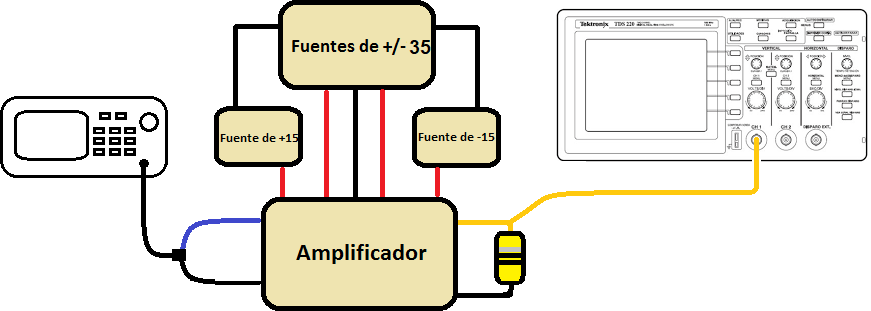
\includegraphics[width= 0.8 \textwidth]{./img/bancos/banco_BW.png}
    \caption{Banco de medición para el ancho de banda.}
    \label{fig:banco_BW}
\end{figure}



Para la medición del ancho de banda, se buscaron las frecuencias de corte para una señal tal que sea alrededor del $10 \si[per-mode=symbol]{\percent}$ o $15 \si[per-mode=symbol]{\percent}$ de la potencia máxima de $40 \si[per-mode=symbol]{\watt}$ especificada. Por lo tanto, se obtiene que la tensión de salida deberá tener un valor de $v_{out} = 8.9 \si[per-mode=symbol]{\volt}$, y las frecuencias de corte se determinaran cuando $v_{out} \approx 8.48 \si[per-mode=symbol]{\volt}$.

Se pueden observar los resultados de la medición en el cuadro ~\tableref{tab:BW_low_power}.


\begin{table}[H]  %%\centering
    
    \setlength\arrayrulewidth{1.5pt}
    \arrayrulecolor{white}
    \def\clinecolor{\hhline{|>{\arrayrulecolor{white}}-%
    >{\arrayrulecolor{white}}|-|-|-|-|}}
    
\begin{center}  
\resizebox{0.7 \textwidth}{!}{%    
\begin{tabularx}{1 \textwidth}%
    {|
    >{\columncolor{white} \centering\arraybackslash}m{0.3333\linewidth}
     |
    >{\columncolor{white} \centering\arraybackslash}m{0.1667\linewidth}
     |
    >{\columncolor{white} \centering\arraybackslash}m{0.1667\linewidth}
     |
    >{\columncolor{white} \centering\arraybackslash}m{0.1667\linewidth}
     |
    }
    \rowcolor{HeadersColor} \thead{Frecuencia} & \thead{$V_{out}$} & \thead{$P$} & \thead{Fase}\\    
    \hhline{|-|-|-|-|}
    %\rowcolor{Butter!20} \cellcolor{Butter!40} $I_{C}$ [$\si[per-mode=symbol]{\milli\ampere}$] & $0.54$ & $8.66$ & $9$ & $6$ & $5.5$ & $10$ & $10$  \\
    \rowcolor{gray!20} \cellcolor{gray!40} $10 \si[per-mode=symbol]{\hertz}$      & $7.2 \si[per-mode=symbol]{\volt}$ & $3.24 \si[per-mode=symbol]{\watt}$ & $38.9 \si[per-mode=symbol]{\degree}$  \\
    \hhline{|-|-|-|-|}   
    \rowcolor{gray!20} \cellcolor{gray!40} $17.32 \si[per-mode=symbol]{\hertz}$   & $8.4 \si[per-mode=symbol]{\volt}$ & $4.41 \si[per-mode=symbol]{\watt}$ & $23.13 \si[per-mode=symbol]{\degree}$ \\
    \hhline{|-|-|-|-|}   
    \rowcolor{gray!20} \cellcolor{gray!40} $100 \si[per-mode=symbol]{\hertz}$     & $8.9 \si[per-mode=symbol]{\volt}$ & $5 \si[per-mode=symbol]{\watt}$ & $0 \si[per-mode=symbol]{\degree}$ \\
    \hhline{|-|-|-|-|}  
    \rowcolor{gray!20} \cellcolor{gray!40} $1 \si[per-mode=symbol]{\kilo\hertz}$      & $8.9 \si[per-mode=symbol]{\volt}$ & $5 \si[per-mode=symbol]{\watt}$ & $0 \si[per-mode=symbol]{\degree}$ \\
    \hhline{|-|-|-|-|}
    \rowcolor{gray!20} \cellcolor{gray!40} $10 \si[per-mode=symbol]{\kilo\hertz}$     & $8.9 \si[per-mode=symbol]{\volt}$ & $5 \si[per-mode=symbol]{\watt}$ & $0 \si[per-mode=symbol]{\degree}$ \\
    \hhline{|-|-|-|-|}  
    \rowcolor{gray!20} \cellcolor{gray!40} $42.3 \si[per-mode=symbol]{\kilo\hertz}$   & $8.4 \si[per-mode=symbol]{\volt}$ & $4.41 \si[per-mode=symbol]{\watt}$ & $0.12 \si[per-mode=symbol]{\degree}$ \\
    \hhline{|-|-|-|-|}      
    \rowcolor{gray!20} \cellcolor{gray!40} $100 \si[per-mode=symbol]{\kilo\hertz}$    & $8 \si[per-mode=symbol]{\volt}$   & $4 \si[per-mode=symbol]{\watt}$ & $29.52 \si[per-mode=symbol]{\degree}$ \\
    \hhline{|-|-|-|-|}                          
    \end{tabularx}}
    \caption{Valores significativos del ancho de banda a baja potencia.}
    \label{tab:BW_low_power}
	\end{center}
\end{table}







En el cuadro~\tableref{tab:comp_BW_low_power} se comparan los ancho de banda obtenidos por simulación, los medidos y los especificados:



\begin{table}[H]  %%\centering
    
    \setlength\arrayrulewidth{1.5pt}
    \arrayrulecolor{white}
    \def\clinecolor{\hhline{|>{\arrayrulecolor{white}}-%
    >{\arrayrulecolor{white}}|-|-|-|-|}}
    
\begin{center}  
\resizebox{0.7 \textwidth}{!}{%    
\begin{tabularx}{1 \textwidth}%
    {|
    >{\columncolor{white} \centering\arraybackslash}m{0.3333\linewidth}
     |
    >{\columncolor{white} \centering\arraybackslash}m{0.1667\linewidth}
     |
    >{\columncolor{white} \centering\arraybackslash}m{0.1667\linewidth}
     |
    >{\columncolor{white} \centering\arraybackslash}m{0.3333\linewidth}
     |
    }
    \rowcolor{HeadersColor} \thead{Valor} & \thead{Especificación} & \thead{Simulación} & \thead{Medición}\\    
    \hhline{|-|-|-|-|}
    %\rowcolor{Butter!20} \cellcolor{Butter!40} $I_{C}$ [$\si[per-mode=symbol]{\milli\ampere}$] & $0.54$ & $8.66$ & $9$ & $6$ & $5.5$ & $10$ & $10$  \\
    \rowcolor{gray!20} \cellcolor{gray!40} $f_{l}$ & $10 \si[per-mode=symbol]{\hertz}$ & $22.34 \si[per-mode=symbol]{\hertz}$ & $17.32 \si[per-mode=symbol]{\hertz}$ \\
    \hhline{|-|-|-|-|}   
    \rowcolor{gray!20} \cellcolor{gray!40} $f_{h}$ & $50 \si[per-mode=symbol]{\kilo\hertz}$ & $97.92 \si[per-mode=symbol]{\kilo\hertz}$ & $42.3 \si[per-mode=symbol]{\kilo\hertz}$ \\
    \hhline{|-|-|-|-|}         
    \end{tabularx}}
    \caption{Comparación de ancho de banda a baja potencia.}
    \label{tab:comp_BW_low_power}
	\end{center}
\end{table}


\vfill
\clearpage



En la figura ~\figref{fig:BW_low_power_fl} se muestra la medición para el valor de $f_{l}$ para baja potencia, y en las figuras ~\figref{fig:BW_low_power_fl_phase} y ~\figref{fig:BW_low_power_fh_phase}, se muestran las mediciones para el cálculo de la fase de corrimiento de las señales.


\begin{figure}[H]
    \centering
    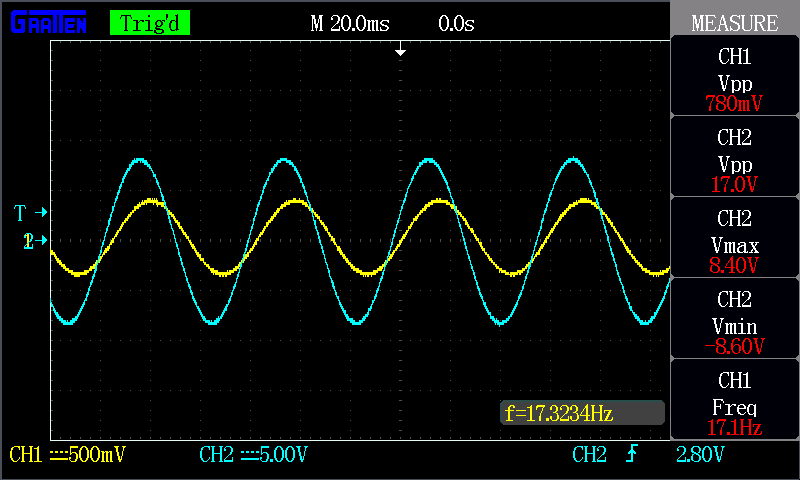
\includegraphics[width=0.95 \textwidth]{./img/mediciones/BW_low_power/1.png}
    \caption{Medición de $f_{l}$ a baja potencia, mostrando el corrimiento de fase.}
    \label{fig:BW_low_power_fl}
\end{figure}


\vfill
\clearpage

\begin{figure}[H]
    \centering
    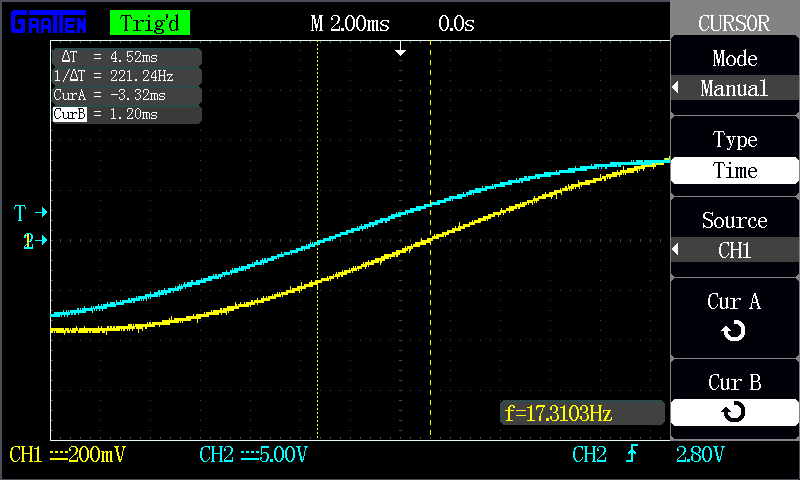
\includegraphics[width=0.95 \textwidth]{./img/mediciones/BW_low_power/3.png}
    \caption{Cálculo del corrimiento de fase para $f_{l}$ a baja potencia.}
    \label{fig:BW_low_power_fl_phase}
\end{figure}

\begin{figure}[H]
    \centering
    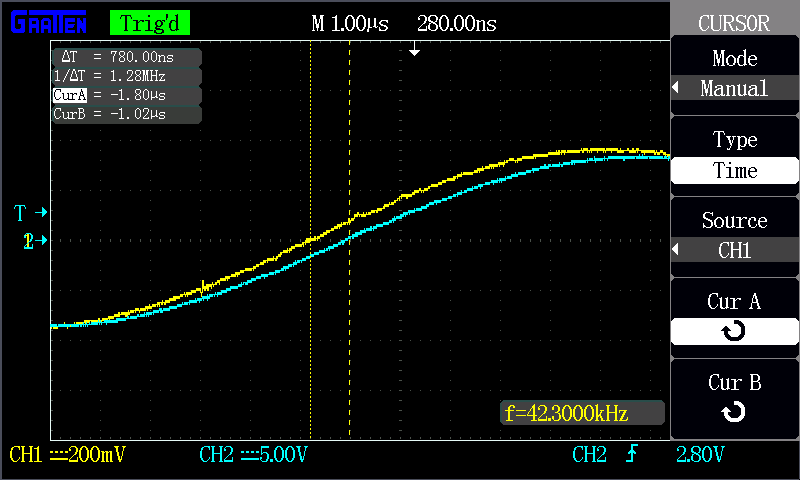
\includegraphics[width=0.95 \textwidth]{./img/mediciones/BW_low_power/4.png}
    \caption{Cálculo del corrimiento de fase para $f_{h}$ a baja potencia.}
    \label{fig:BW_low_power_fh_phase}
\end{figure}

\vfill
\clearpage


\subsubsection{Ancho de banda de potencia}

Se usó para la medición, el banco de medición de la medición anterior, mostrado en la figura~\figref{fig:banco_BW}, usando los instrumentos detallados en la sección~\sectref{sec:instrumentos}.


 Para el caso del ancho de banda de potencia, se repite el procedimiento de la sección anterior pero con una señal de salida $V_{out} = 25.3 \si[per-mode=symbol]{\volt}$ a máxima potencia ($40 \si[per-mode=symbol]{\watt}$). En este caso, las frecuencias de corte se determinan cuando $V_{out} = 24 \si[per-mode=symbol]{\volt}$, tomando como en el caso anterior las frecuencias de corte al $10 \si[per-mode=symbol]{\percent}$.\\
Se pueden observar los resultados de la medición en el cuadro ~\tableref{tab:BW_power}.


\begin{table}[H]  %%\centering
    
    \setlength\arrayrulewidth{1.5pt}
    \arrayrulecolor{white}
    \def\clinecolor{\hhline{|>{\arrayrulecolor{white}}-%
    >{\arrayrulecolor{white}}|-|-|-|-|}}
    
\begin{center}  
\resizebox{0.7 \textwidth}{!}{%    
\begin{tabularx}{1 \textwidth}%
    {|
    >{\columncolor{white} \centering\arraybackslash}m{0.3333\linewidth}
     |
    >{\columncolor{white} \centering\arraybackslash}m{0.1667\linewidth}
     |
    >{\columncolor{white} \centering\arraybackslash}m{0.1667\linewidth}
     |
    >{\columncolor{white} \centering\arraybackslash}m{0.1667\linewidth}
     |
    }
    \rowcolor{HeadersColor} \thead{Frecuencia} & \thead{$V_{out}$} & \thead{$P$} & \thead{Fase}\\    
    \hhline{|-|-|-|-|}
    %\rowcolor{Butter!20} \cellcolor{Butter!40} $I_{C}$ [$\si[per-mode=symbol]{\milli\ampere}$] & $0.54$ & $8.66$ & $9$ & $6$ & $5.5$ & $10$ & $10$  \\
    \rowcolor{gray!20} \cellcolor{gray!40} $10 \si[per-mode=symbol]{\hertz}$      & $20.8 \si[per-mode=symbol]{\volt}$ & $27.09 \si[per-mode=symbol]{\watt}$ & $49.32 \si[per-mode=symbol]{\degree}$  \\
    \hhline{|-|-|-|-|}   
    \rowcolor{gray!20} \cellcolor{gray!40} $19.75 \si[per-mode=symbol]{\hertz}$   & $24 \si[per-mode=symbol]{\volt}$ & $4.41 \si[per-mode=symbol]{\watt}$ & $24.56 \si[per-mode=symbol]{\degree}$ \\
    \hhline{|-|-|-|-|}   
    \rowcolor{gray!20} \cellcolor{gray!40} $100 \si[per-mode=symbol]{\hertz}$     & $25.3 \si[per-mode=symbol]{\volt}$ & $5 \si[per-mode=symbol]{\watt}$ & $0 \si[per-mode=symbol]{\degree}$ \\
    \hhline{|-|-|-|-|}  
    \rowcolor{gray!20} \cellcolor{gray!40} $1 \si[per-mode=symbol]{\kilo\hertz}$      & $25.3 \si[per-mode=symbol]{\volt}$ & $5 \si[per-mode=symbol]{\watt}$ & $0 \si[per-mode=symbol]{\degree}$ \\
    \hhline{|-|-|-|-|}
    \rowcolor{gray!20} \cellcolor{gray!40} $10 \si[per-mode=symbol]{\kilo\hertz}$     & $25.3 \si[per-mode=symbol]{\volt}$ & $5 \si[per-mode=symbol]{\watt}$ & $0 \si[per-mode=symbol]{\degree}$ \\
    \hhline{|-|-|-|-|}  
    \rowcolor{gray!20} \cellcolor{gray!40} $37.54 \si[per-mode=symbol]{\kilo\hertz}$   & $24 \si[per-mode=symbol]{\volt}$ & $4.41 \si[per-mode=symbol]{\watt}$ & $23.09 \si[per-mode=symbol]{\degree}$ \\
    \hhline{|-|-|-|-|}                          
    \end{tabularx}}
    \caption{Valores significativos del ancho de banda a máxima potencia.}
    \label{tab:BW_power}
	\end{center}
\end{table}



En el cuadro ~\tableref{tab:comp_BW_power} se comparan los anchos de banda obtenidos por simulación, los medidos y los especificados:



\begin{table}[H]  %%\centering
    
    \setlength\arrayrulewidth{1.5pt}
    \arrayrulecolor{white}
    \def\clinecolor{\hhline{|>{\arrayrulecolor{white}}-%
    >{\arrayrulecolor{white}}|-|-|-|-|}}
    
\begin{center}  
\resizebox{0.7 \textwidth}{!}{%    
\begin{tabularx}{1 \textwidth}%
    {|
    >{\columncolor{white} \centering\arraybackslash}m{0.3333\linewidth}
     |
    >{\columncolor{white} \centering\arraybackslash}m{0.1667\linewidth}
     |
    >{\columncolor{white} \centering\arraybackslash}m{0.1667\linewidth}
     |
    >{\columncolor{white} \centering\arraybackslash}m{0.3333\linewidth}
     |
    }
    \rowcolor{HeadersColor} \thead{Valor} & \thead{Especificación} & \thead{Simulación} & \thead{Medición}\\    
    \hhline{|-|-|-|-|}
    %\rowcolor{Butter!20} \cellcolor{Butter!40} $I_{C}$ [$\si[per-mode=symbol]{\milli\ampere}$] & $0.54$ & $8.66$ & $9$ & $6$ & $5.5$ & $10$ & $10$  \\
    \rowcolor{gray!20} \cellcolor{gray!40} $f_{l}$ & $-$ & $22.34 \si[per-mode=symbol]{\hertz}$ & $19.75 \si[per-mode=symbol]{\hertz}$ \\
    \hhline{|-|-|-|-|}   
    \rowcolor{gray!20} \cellcolor{gray!40} $f_{h}$ & $30 \si[per-mode=symbol]{\kilo\hertz}$ & $97.84 \si[per-mode=symbol]{\kilo\hertz}$ & $37.54 \si[per-mode=symbol]{\kilo\hertz}$ (Limitado por \textit{Slew-Rate}) \\
    \hhline{|-|-|-|-|}         
    \end{tabularx}}
    \caption{Comparación de ancho de banda a máxima potencia.}
    \label{tab:comp_BW_power}
	\end{center}
\end{table}



En las figura~\figref{fig:BW_power_fl_phase} y la figura~\figref{fig:BW_power_fh_phase}, se muestran las mediciones para el cálculo de la fase de corrimiento de las señales.


\vfill
\clearpage


\begin{figure}[H]
    \centering
    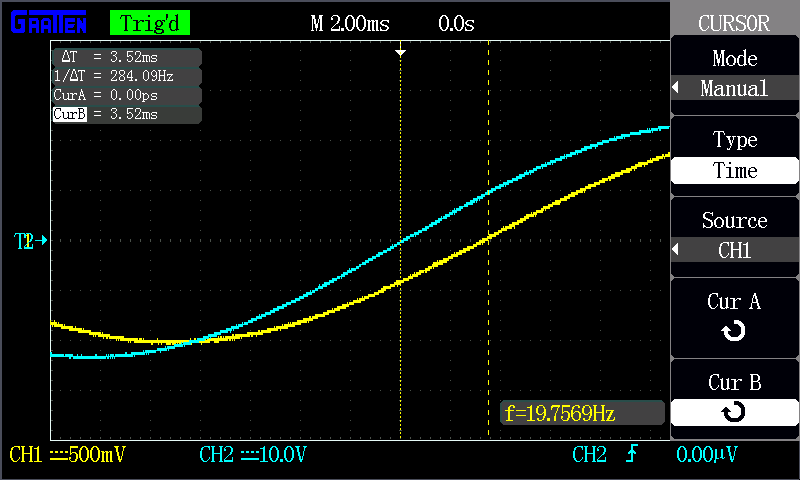
\includegraphics[width=0.95 \textwidth]{./img/mediciones/BW_power/3.png}
    \caption{Medición de $f_l$ a máxima potencia, mostrando el corrimiento de fase.}
    \label{fig:BW_power_fl_phase}
\end{figure}


\begin{figure}[H]
    \centering
    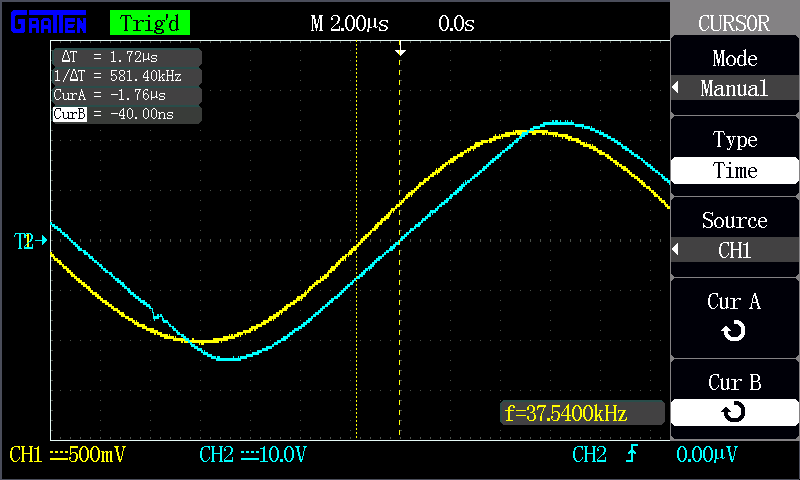
\includegraphics[width=0.95 \textwidth]{./img/mediciones/BW_power/4.png}
    \caption{Medición de $f_l$ a máxima potencia, mostrando el corrimiento de fase.}
    \label{fig:BW_power_fh_phase}
\end{figure}



\vfill
\clearpage


\subsubsection{Impedancias de entrada y salida}

Se armó para la primer medición, el banco de medición mostrado en la figura~\figref{fig:banco_Ri}, usando los instrumentos detallados en la sección~\sectref{sec:instrumentos} y para la segunda medición se utilizó únicamente el multímetro \textit{true-rms}, figura~\figref{fig:multimeter_lab}.


\begin{figure}[H]
    \centering
    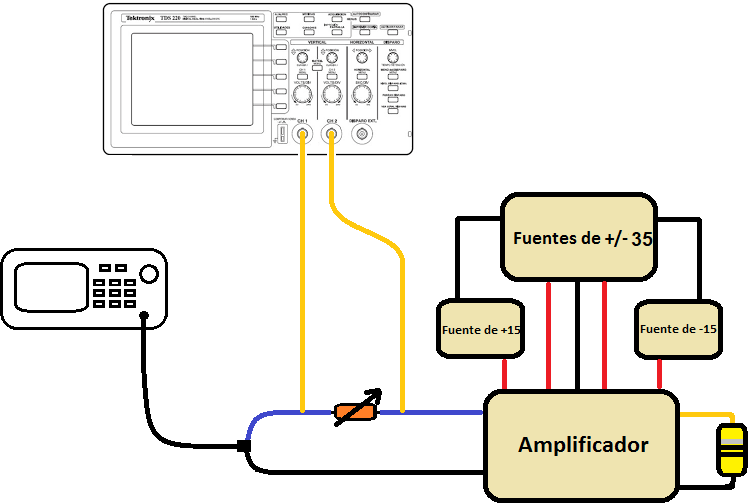
\includegraphics[width= 0.8 \textwidth]{./img/bancos/banco_Ri.png}
    \caption{Banco de medición para el ancho de banda.}
    \label{fig:banco_Ri}
\end{figure}







Para la impedancia de entrada, se colocó en serie con el generador, un resistor variable. El mismo fue ajustado de forma tal que la tensión de salida fijada por el generador, disminuya a la mitad a la entrada del amplificador. El método se realizó para $\num 3$ frecuencias distintas ( $100 \si[per-mode=symbol]{\hertz}$, $1 \si[per-mode=symbol]{\kilo\hertz}$ y  $10 \si[per-mode=symbol]{\kilo\hertz}$), obteniéndose de este modo $z_{in} = 21.56\si[per-mode=symbol]{\kilo\ohm}$ para las tres mediciones.\\

Para el caso de la resistencia de salida, se determina su valor midiendo la tensión dos veces, una en vacío ($V_{out}$) y otra con carga nominal ($V_c$), a una frecuencia de $1 \si[per-mode=symbol]{\kilo\hertz}$ y una amplitud tal que permita obtener la lectura de mayor resolución posible en el voltímetro utilizado. Luego, la impedancia de salida se calcula mediante la ecuación~\eqref{eq:z_out}:

\begin{equation}
    z_{out} = R_c \cdot \left( \frac{V_{out}}{V_c}-1 \right)
    \label{eq:z_out}
\end{equation}

Los valores obtenidos fueron $V_{out} = 17.57 \si[per-mode=symbol]{\volt}$, $V_c= 17.39 \si[per-mode=symbol]{\volt}$ con $R_c = 6.58\si[per-mode=symbol]{\ohm}$, obteniéndose como resultado $z_{out} = 68.10\si[per-mode=symbol]{\milli\ohm}$.\\

Se muestra en el cuadro ~\tableref{tab:comp_impedance} la comparación para los distintos valores de impedancia obtenidos a $1 \si[per-mode=symbol]{\kilo\hertz}$:


\begin{table}[H]  %%\centering
    
    \setlength\arrayrulewidth{1.5pt}
    \arrayrulecolor{white}
    \def\clinecolor{\hhline{|>{\arrayrulecolor{white}}-%
    >{\arrayrulecolor{white}}|-|-|-|-|}}
    
\begin{center}  
\resizebox{0.7 \textwidth}{!}{%    
\begin{tabularx}{1 \textwidth}%
    {|
    >{\columncolor{white} \centering\arraybackslash}m{0.3333\linewidth}
     |
    >{\columncolor{white} \centering\arraybackslash}m{0.1667\linewidth}
     |
    >{\columncolor{white} \centering\arraybackslash}m{0.1667\linewidth}
     |
    >{\columncolor{white} \centering\arraybackslash}m{0.3333\linewidth}
     |
    }
    \rowcolor{HeadersColor} \thead{Valor} & \thead{Especificación} & \thead{Simulación} & \thead{Medición}\\    
    \hhline{|-|-|-|-|}
    %\rowcolor{Butter!20} \cellcolor{Butter!40} $I_{C}$ [$\si[per-mode=symbol]{\milli\ampere}$] & $0.54$ & $8.66$ & $9$ & $6$ & $5.5$ & $10$ & $10$  \\
    \rowcolor{gray!20} \cellcolor{gray!40} $z_{in}$ & $22\si[per-mode=symbol]{\kilo\ohm}$ & $21.99 \si[per-mode=symbol]{\kilo\ohm}$ & $21.88 \si[per-mode=symbol]{\kilo\ohm}$ \\
    \hhline{|-|-|-|-|}   
    \rowcolor{gray!20} \cellcolor{gray!40} $z_{out}$ & $\approx 0$ & $0.87 \si[per-mode=symbol]{\milli\ohm}$ & $68.10 \si[per-mode=symbol]{\milli\ohm}$ \\
    \hhline{|-|-|-|-|}         
    \end{tabularx}}
    \caption{Comparación de impedancias de entrada y salida (a 1 \si[per-mode=symbol]{\kilo\hertz})}
    \label{tab:comp_impedance}
	\end{center}
\end{table}

Una cosa a destacar de esta medición, es que su precisión se vio afectada por la precisión del voltímetro con el que se disponía, y que además en el caso de la impedancia de entrada se trata prácticamente de una resistencia en todo el ancho de banda, solo afectada a bajas frecuencias por el acople capacitivo, pero la impedancia de salida, tal como se vio en las simulaciones tiene el desfasaje de una inductancia, el cual no se tiene en cuenta en el método de medición, que toma solo los valores eficaces de las tensiones.

\vfill

\clearpage



\subsubsection{Sensibilidad}

Ya que la red de realimentación de nuestro amplificador está formada por un resistor fijo y un preset, la sensibilidad es ajustable en cierto rango, por lo tanto, la misma se ajustó para obtener lo que se especificó en el diseño, una sensibilidad de $1 \si[per-mode=symbol]{\volt}$. \\
Para verificar esto, se midió el valor eficaz de una señal senoidal de $1 \si[per-mode=symbol]{\kilo\hertz}$ aplicada a la entrada $v_{in}=1.08 \si[per-mode=symbol]{\volt}$, que produce la potencia especificada a la salida con carga nominal, siendo esta última $v_{out}= 25.3 \si[per-mode=symbol]{\volt}$. Se verifica dicha medición en la figura ~\figref{fig:Sensitivity}.

\begin{figure}[H]
    \centering
    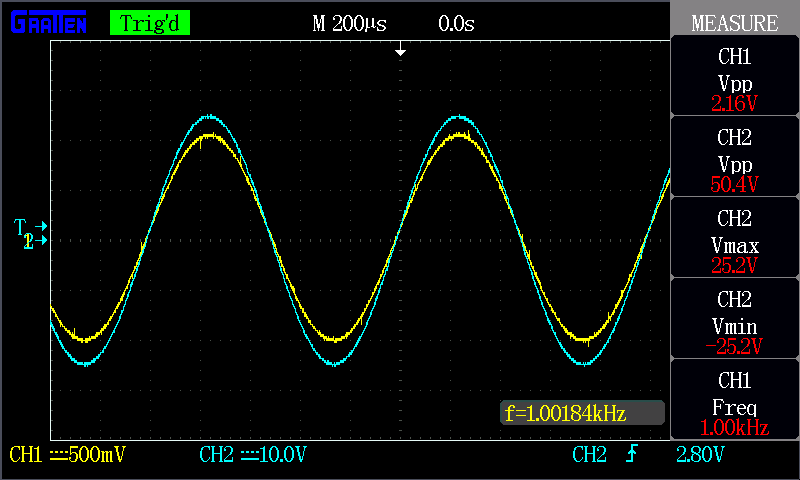
\includegraphics[width=0.95 \textwidth]{./img/mediciones/Sensitivity/1.png}
    \caption{Medición de la sensibilidad del circuito amplificador.}
    \label{fig:Sensitivity}
\end{figure}

\clearpage




\subsubsection{Estabilidad}

Se armó para esta medición, el banco de medición mostrado en la figura~\figref{fig:banco_salida}, usando los instrumentos detallados en la sección~\sectref{sec:instrumentos}.

\begin{figure}[H]
    \centering
    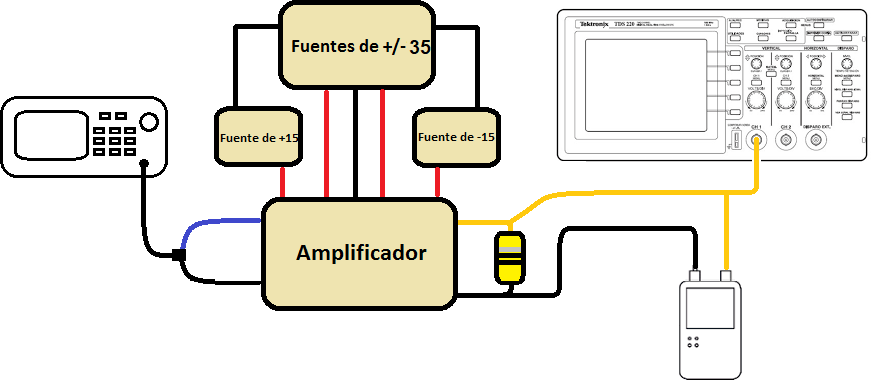
\includegraphics[width= 0.8 \textwidth]{./img/bancos/banco_salida.png}
    \caption{Banco de medición para medir la estabilidad.}
    \label{fig:banco_salida}
\end{figure}


Para evaluar la estabilidad del amplificador, se realizaron mediciones de la salida cuando la entrada es una onda cuadrada, para esta medición se usó una entrada cuadrada de $1 \si[per-mode=symbol]{\kilo\hertz}$ de frecuencia y una amplitud que se ajustó para dos condiciones de potencia, media potencia y máxima potencia, tomando valores \textit{RMS} de salida, en la figura~\figref{fig:estab1} se puede ver lo medido para la entrada y salida para una potencia de aproximadamente $29 \si[per-mode=symbol]{\watt}$ y en la en la figura~\figref{fig:estab2} se puede ver lo medido para la entrada y salida para una potencia de aproximadamente $40 \si[per-mode=symbol]{\watt}$. Puede apreciarse como no hay sobre-picos a la salida que evidencien inestabilidad en el amplificador.

\vfill

\clearpage



\begin{figure}[H]
        \centering
        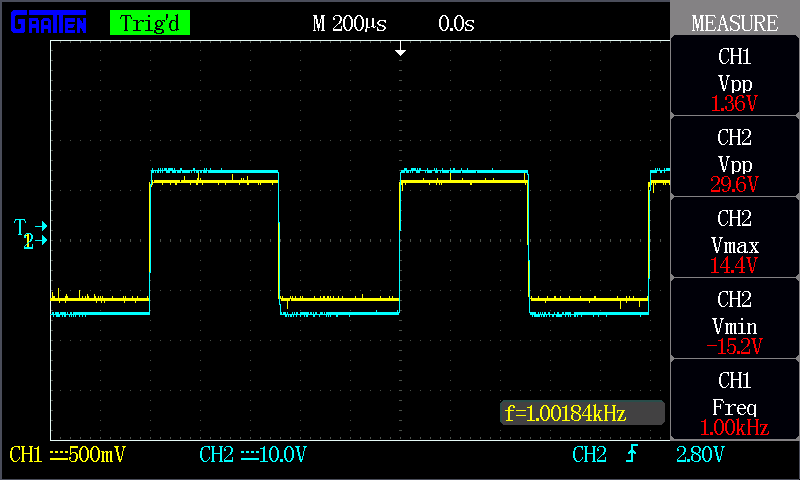
\includegraphics[width=0.95 \textwidth]{./img/mediciones/Power/1.png}
        \caption{Medición del amplificador con una entrada cuadrada de $1 \si[per-mode=symbol]{\kilo\hertz}$ a media potencia.}
        \label{fig:estab1}
\end{figure}


\begin{figure}[H]
        \centering
        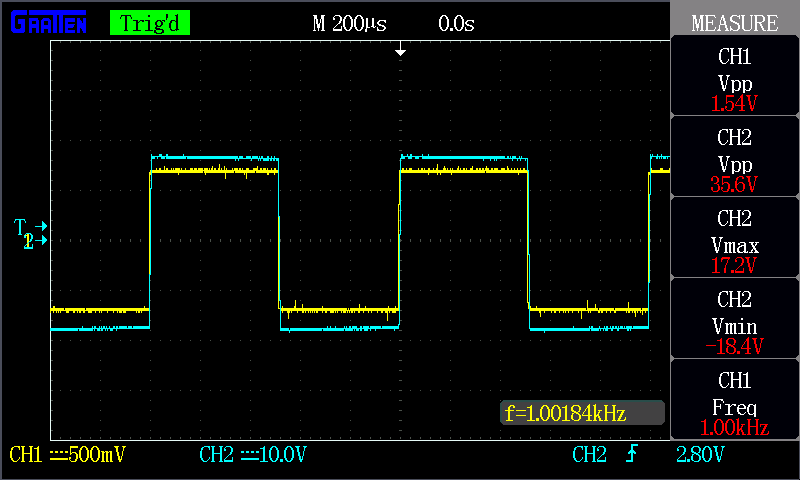
\includegraphics[width=0.95 \textwidth]{./img/mediciones/Power/2.png}
        \caption{Medición del amplificador con una entrada cuadrada de $1 \si[per-mode=symbol]{\kilo\hertz}$ a máxima potencia.}
        \label{fig:estab2}
\end{figure}

\vfill

\clearpage

\subsubsection{Switcheo en la etapa de salida}

Para está medición el banco de medición utilizado es el mismo que en la medición anterior, sin embargo no se realizó con el mismo osciloscopio mostrado en la sección~\sectref{sec:instrumentos} por falta de disponibilidad, el mismo no contaba con captura de datos, y las fotos se tomaron usando la cámara de un celular, en las mismas puede verse marca y modelo.\\

En esta medición se midió las señales presentes en los colectores de los transistores de potencia de salida internos, para ver su forma, en la figura~\figref{fig:switch1} y en la figura~\figref{fig:switch2}, pueden verse las formas de onda para el transistor NPN y el PNP respectivamente. Las mediciones se realizaron a $1 \si[per-mode=symbol]{\kilo\hertz}$. Se observa que las formas son muy cercanas a las esperadas para ambas señales.\\


\vfill

\clearpage


\begin{figure}[H]
        \centering
        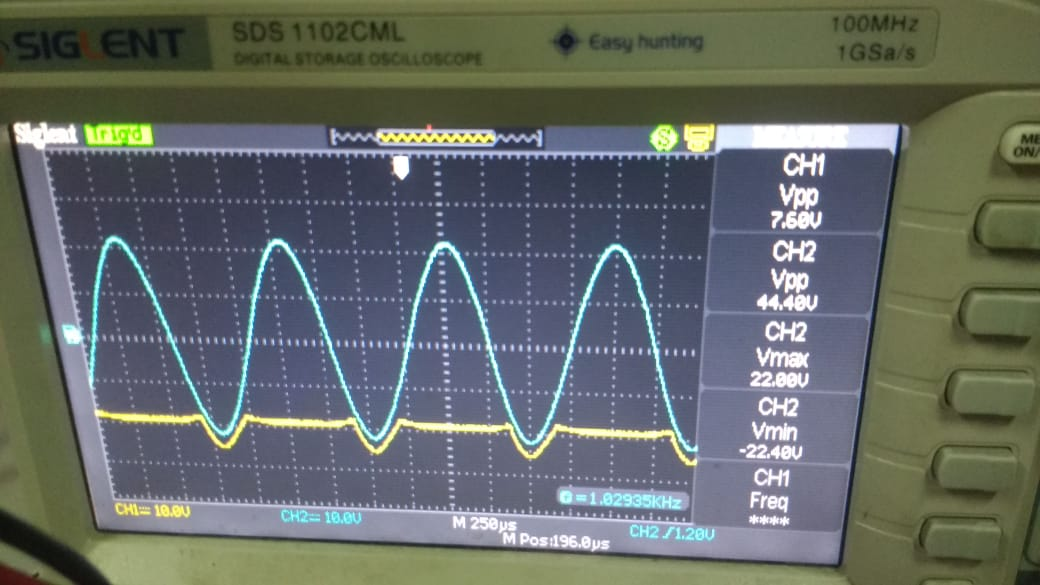
\includegraphics[width=0.95 \textwidth]{./img/mediciones/Switching/1.jpeg}
        \caption{Forma de onda para el transistor \textit{NPN}.}
        \label{fig:switch1}
\end{figure}

\begin{figure}[H]
        \centering
        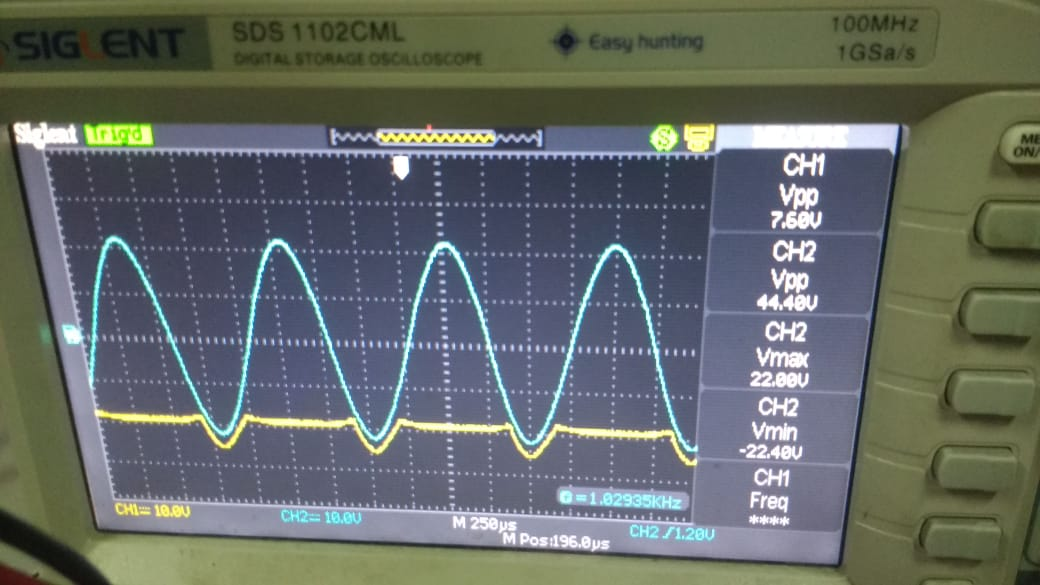
\includegraphics[width=0.95 \textwidth]{./img/mediciones/Switching/1.jpeg}
        \caption{Forma de onda para el transistor \textit{PNP}.}
        \label{fig:switch2}
\end{figure}


\vfill

\clearpage

\subsubsection{THD}

Se armó para la medición, el banco de medición mostrado en la figura~\figref{fig:banco_THD}, usando los instrumentos detallados en la sección~\sectref{sec:instrumentos} y un atenuador formado con un resistor de $3.3 \si[per-mode=symbol]{\kilo\ohm}$ y un preset de $500 \si[per-mode=symbol]{\ohm}$, de manera de poder atenuar desde el valor de máxima excursión a máxima potencia, $25.3 \si[per-mode=symbol]{\volt}$, a un valor menor a $1 \si[per-mode=symbol]{\volt}$, necesario para ingresar por la entrada de línea de la placa de sonido de la PC en forma segura, los valores también se seleccionaron de manera de no cargar al amplificador, ya que el valor $3.3 \si[per-mode=symbol]{\kilo\ohm}$ es despreciable frente a los $8 \si[per-mode=symbol]{\ohm}$ de la carga. El multímetro se usó para verificar la atenuación, luego se retiró al medir el THD.


\begin{figure}[H]
    \centering
    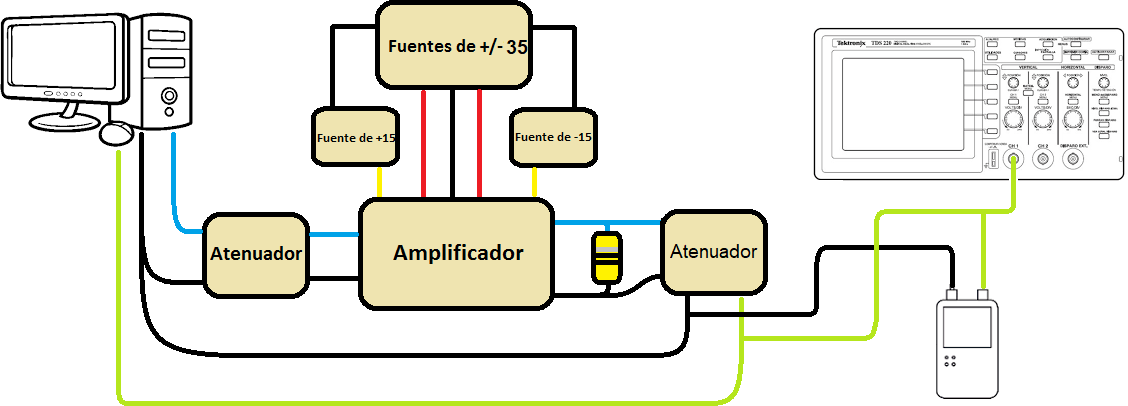
\includegraphics[width= 0.8 \textwidth]{./img/bancos/banco_THD.png}
    \caption{Banco de medición para el THD.}
    \label{fig:banco_THD}
\end{figure}



Una vez conectado el banco se ajustó el atenuador de modo de lograr la menor lectura de THD, manteniendo la máxima excursión en el amplificador se procedió a barrer todo el ancho de banda de audio para obtener la variación del THD en función de la frecuencia.\\
De la figura~\figref{fig:THD900Hz} a la figura~\figref{fig:THD18khz} se muestran algunas de las capturas que fueron tomadas durante las mediciones con el programa \textbf{\textit{Spectra Plus}}.\\
Los valores se recabaron desde $10 \si[per-mode=symbol]{\hertz}$ con saltos de $10 \si[per-mode=symbol]{\hertz}$, hasta alcanzar los $100 \si[per-mode=symbol]{\hertz}$, luego con saltos de $100 \si[per-mode=symbol]{\hertz}$, hasta alcanzar $1 \si[per-mode=symbol]{\kilo\hertz}$, y finalmente con saltos de $1 \si[per-mode=symbol]{\kilo\hertz}$, hasta alcanzar los $19 \si[per-mode=symbol]{\kilo\hertz}$, máxima frecuencia a la que se pudo obtener una medición confiable y repetible. El resultado de estas mediciones se graficó usando \textbf{\textit{MATLAB}}, el mismo se puede ver en la figura~\figref{fig:THD_vs_freq}, contrastado con lo obtenido por simulación, se puede observar como la forma general es aproximadamente correcta, pero los valores medidos son alrededor de $\num 10$ veces mas grandes, especialmente a altas frecuencias, parte de esta diferencia se debe a que las mediciones incluyen ruido, y también a las reactancias distribuidas en el circuito y los semiconductores que las simulaciones no contemplan, otras fuentes de la diferencias, son el propio método de ventaneo y \textit{FFT} usado por el programa. También se observan algunos puntos anómalos, donde probablemente la medición no se hizo correctamente.\\


Luego de relevar el THD en función de la frecuencia, se procedió a hacer lo mismo respecto a la potencia de salida del amplificador, para esto, usando el mismo banco de medición, pero ahora utilizando en lugar de la señal generada por la PC, el generador senoidal mostrado en la figura~\figref{fig:signalgen2_lab}, el motivo de esto, es que el volumen de la PC no permitía un ajuste preciso de la intensidad de la salida y el atenuador de entrada solo permitía un rango limitado. De el generador se tomó una señal de $1 \si[per-mode=symbol]{\kilo\hertz}$, y se ajustó su salida para lograr a la salida del amplificador sobre la carga potencias en pasos de $1 \si[per-mode=symbol]{\watt}$, los valores que se recabaron se pueden ver en un gráfico realizado en \textbf{\textit{MATLAB}}, figura~\figref{fig:THD_vs_power}, donde se contrastan los mismos con lo obtenido por simulación, para poder ver ambos gráficos en la misma figura, el eje de abscisas del gráfico de la simulación esta escalado en $\num 10$ veces, observando nuevamente este orden de diferencia entre lo medido y lo simulado. A bajas potencias las mediciones parecen ser un poco erráticas, esto se debe mas que todo al hecho de que a bajas amplitudes de salida el atenuador se tuvo que ajustar para lograr mediciones del programa, pero a estos niveles el ruido tiene mucho mas peso.



\clearpage


\begin{figure}[H]
    \centering
    \includegraphics[width=0.95 \textwidth, angle=0]{img/mediciones/THD/900hz.png}
    \caption{Medición del THD a $900 \si[per-mode=symbol]{\hertz}$.}
    \label{fig:THD900Hz}
\end{figure}


\begin{figure}[H]
    \centering
    \includegraphics[width=0.95 \textwidth, angle=0]{img/mediciones/THD/1khz.png}
    \caption{Medición del THD a $1 \si[per-mode=symbol]{\kilo\hertz}$.}
    \label{fig:THD1kHz}
\end{figure}

\clearpage



\begin{figure}[H]
    \centering
    \includegraphics[width=0.95 \textwidth, angle=0]{img/mediciones/THD/2khz.png}
    \caption{Medición del THD a $2 \si[per-mode=symbol]{\kilo\hertz}$.}
    \label{fig:THD2khz}
\end{figure}



\begin{figure}[H]
    \centering
    \includegraphics[width=0.95 \textwidth, angle=0]{img/mediciones/THD/9khz.png}
    \caption{Medición del THD a $9 \si[per-mode=symbol]{\kilo\hertz}$.}
    \label{fig:THD9KHz}
\end{figure}


\clearpage


\begin{figure}[H]
    \centering
    \includegraphics[width=0.95 \textwidth, angle=0]{img/mediciones/THD/17khz.png}
    \caption{Medición del THD a $17 \si[per-mode=symbol]{\kilo\hertz}$.}
    \label{fig:THD17khz}
\end{figure}


\begin{figure}[H]
    \centering
    \includegraphics[width=0.95 \textwidth, angle=0]{img/mediciones/THD/18khz.png}
    \caption{Medición del THD a $18 \si[per-mode=symbol]{\kilo\hertz}$.}
    \label{fig:THD18khz}
\end{figure}



\clearpage



\begin{figure}[H]
    \centering
    \includegraphics[height=0.65 \textwidth, angle=90]{img/mediciones/THD/THD_vs_frequency.png}
    \caption{Medición del THD en función de la frecuencia.}
    \label{fig:THD_vs_freq}
\end{figure}

\clearpage

\begin{figure}[H]
    \centering
    \includegraphics[height=0.65 \textwidth, angle=90]{img/mediciones/THD/THD_vs_power.png}
    \caption{Medición del THD en función de la potencia.}
    \label{fig:THD_vs_power}
\end{figure}

\clearpage


\subsubsection{Slew Rate}

Se aplicó una señal cuadrada de máxima potencia a modo de obtener el valor numérico del SR, calculando la pendiente de la recta obtenida en la figura~\figref{fig:Slew_rate_amplifier}. Antes, se verficó en la figura  ~\figref{fig:Slew_rate_gen} que el tiempo de crecimiento de la fuente generadora de señal sea lo suficientemente baja para poder garantizar una correcta medición, siendo este tiempo de $\tau = 264 \si[per-mode=symbol]{\nano\second}$.


\begin{figure}[H]
        \centering
        \includegraphics[width=0.95 \textwidth]{./img/mediciones/Slew_Rate/1.png}
        \caption{Verificación de tiempo de crecimiento del generador.}
        \label{fig:Slew_rate_gen}
\end{figure}

\vfill

\clearpage

\begin{figure}[H]
        \centering
        \includegraphics[width=0.95 \textwidth]{./img/mediciones/Slew_Rate/2.png}
        \caption{Medición del Slew Rate del circuito amplificador.}
        \label{fig:Slew_rate_amplifier}
\end{figure}

Mediante el cálculo pertinente, y comparando con las simulaciones, se obtiene el cuadro~\tableref{tab:comp_SlewRate}, donde se compara lo medido con la especificación y lo simulado



\begin{table}[H]  %%\centering
    
    \setlength\arrayrulewidth{1.5pt}
    \arrayrulecolor{white}
    \def\clinecolor{\hhline{|>{\arrayrulecolor{white}}-%
    >{\arrayrulecolor{white}}|-|-|-|-|}}
    
\begin{center}  
\resizebox{0.7 \textwidth}{!}{%    
\begin{tabularx}{1 \textwidth}%
    {|
    >{\columncolor{white} \centering\arraybackslash}m{0.3333\linewidth}
     |
    >{\columncolor{white} \centering\arraybackslash}m{0.1667\linewidth}
     |
    >{\columncolor{white} \centering\arraybackslash}m{0.1667\linewidth}
     |
    >{\columncolor{white} \centering\arraybackslash}m{0.1667\linewidth}
     |
    }
    \rowcolor{HeadersColor} \thead{Valor} & \thead{Especificación} & \thead{Simulación} & \thead{Medición}\\    
    \hhline{|-|-|-|-|}
    %\rowcolor{Butter!20} \cellcolor{Butter!40} $I_{C}$ [$\si[per-mode=symbol]{\milli\ampere}$] & $0.54$ & $8.66$ & $9$ & $6$ & $5.5$ & $10$ & $10$  \\
    \rowcolor{gray!20} \cellcolor{gray!40} \textit{Slew Rate} & $5 \si[per-mode=symbol]{\volt\per\micro\second}$ & $4.79 \si[per-mode=symbol]{\volt\per\micro\second}$ & $4.32 \si[per-mode=symbol]{\volt\per\micro\second}$ \\
    \hhline{|-|-|-|-|}       
    \end{tabularx}}
    \caption{Comparación del Slew Rate.}
    \label{tab:comp_SlewRate}
	\end{center}
\end{table}


\vfill

\clearpage


\subsubsection{Rechazo al ripple}


Se armó para la medición, el banco de medición mostrado en la figura~\figref{fig:banco_ripple}, usando los instrumentos detallados en la sección~\sectref{sec:instrumentos}. En el diagrama, el módulo que se conecta entre la alimentación y el amplificador es el circuito para generar ripple propuesto por la cátedra, el mismo se muestra en la figura~\figref{fig:generador_ripple}, este circuito a partir del uso de un \textit{MOSFET} que se dispara con un generador de onda cuadrada con una amplitud de unos $12 \si[per-mode=symbol]{\volt}$ y $20 \si[per-mode=symbol]{\hertz}$, introduce un ripple en la alimentación de aproximadamente unos $3 \si[per-mode=symbol]{\volt}$ de pico. Para lograr esta medición con una precisión adecuada la medición se realizó con el osciloscopio para la entrada, que sería el valor \textit{RMS} de la señal montada sobre la continua de la fuente, ya que esta tiene una amplitud apreciable, usando la medición de valor \textit{RMS} del osciloscopio, se pudo medir sin problema, pero para la salida, la señal es muy pequeña, siendo mas adecuada la medición con el voltímetro \textit{true-rms}, con los valores obtenidos se aplicó la expresión \eqref{eq:ripple_rej}, para la relación de rechazo de ripple expresada en $\si[per-mode=symbol]{\decibel}$.\\
Con esta expresión y usando los valores medidos, $V_{CC_{ripp}} \approx 2.1 \si[per-mode=symbol]{\volt}$ y $V_{o_{ripp}} \approx 10 \si[per-mode=symbol]{\milli\volt}$, se llega al valor obtenido ,bastante cercano a los $-55.63 \si[per-mode=symbol]{\decibel}$ obtenidos por simulación.

\begin{equation}
\boxed{ RR = 20 \cdot Log_{10} \left(  \frac{V_{0_{ripp}}}{V_{CC_{ripp}}} \right) = -45 \si[per-mode=symbol]{\decibel}}
\label{eq:ripple_rej}
\end{equation}


\vfill


\clearpage


\begin{figure}[H]
    \centering
    \includegraphics[width= 0.8 \textwidth]{./img/bancos/banco_Ripple.png}
    \caption{Banco de medición para el rechazo de ripple.}
    \label{fig:banco_ripple}
\end{figure}


\begin{figure}[H]
    \centering
    \includegraphics[width= 0.6 \textwidth]{./img/circuito/PSRR_circ.png}
    \caption{Circuito usado para la generación de ripple.}
    \label{fig:generador_ripple}
\end{figure}


\vfill


\clearpage


\subsubsection{Comportamiento térmico}

Esta medición se realizó usando una termocupla tipo \textit{K}, conectada al multímetro mencionado en la sección~\sectref{sec:instrumentos}, en la escala de medición de temperaturas. \\

Se midió la temperatura del disipador con el multímetro para el caso de máxima potencia. Los resultados en función del tiempo se muestran en el cuadro~\tableref{tab:comp_term}. Luego de aproximadamente $ 30 \si[per-mode=symbol]{\minute} $, la temperatura no presentó variaciones notables. La temperatura sobre las cápsulas de los transistores se estabilizaron en un valor por debajo de las máximas, y no cambiaron tampoco a partir de alcanzado ese valor.



\begin{table}[H]  %%\centering
    
    \setlength\arrayrulewidth{1.5pt}
    \arrayrulecolor{white}
    \def\clinecolor{\hhline{|>{\arrayrulecolor{white}}-%
    >{\arrayrulecolor{white}}|-|-|}}
    
\begin{center}  
\resizebox{0.7 \textwidth}{!}{%    
\begin{tabularx}{1 \textwidth}%
    {|
    >{\columncolor{white} \centering\arraybackslash}m{0.3333\linewidth}
     |
    >{\columncolor{white} \centering\arraybackslash}m{0.3333\linewidth}
     |
    }
    \rowcolor{HeadersColor} \thead{Tiempo} & \thead{Temperatura}\\    
    \hhline{|-|-|}
    \rowcolor{gray!20}  $ 5 \si[per-mode=symbol]{\minute} $ & $ 33 \si[per-mode=symbol]{\degree\celsius} $ \\
    \hhline{|-|-|}   
    \rowcolor{gray!20}  $ 15 \si[per-mode=symbol]{\minute} $ & $ 33 \si[per-mode=symbol]{\degree\celsius} $ \\
    \hhline{|-|-|}   
    \rowcolor{gray!20}  $ 30 \si[per-mode=symbol]{\minute} $ & $ 38 \si[per-mode=symbol]{\degree\celsius} $ \\
    \hhline{|-|-|}   
    \rowcolor{gray!20}  $ 45 \si[per-mode=symbol]{\minute} $ & $ 40 \si[per-mode=symbol]{\degree\celsius} $ \\
    \hhline{|-|-|}   
    \rowcolor{gray!20}  $ 60 \si[per-mode=symbol]{\minute} $ & $ 45 \si[per-mode=symbol]{\degree\celsius} $ \\
    \hhline{|-|-|}            
    \end{tabularx}}
    \caption{Temperatura del disipador a máxima potencia de salida ($ T_{amb} = 27 \si[per-mode=symbol]{\degree\celsius} $).}
    \label{tab:comp_term}
	\end{center}
\end{table}



\clearpage
%%\\\\\\\\\\\\\\\\\\\\\\\\\\\



%\subsection{Diagramas de conexionado}
%El siguiente diagrama muestra como se conectaría la fuente [seccion~\ref{sec:fuente}], el amplificador y el parlante.
%
%\begin{figure}[H]
%\centering
%\includegraphics[width=1\textwidth]{img/integracion/diagrama_completo}
%\caption{Diagrama completo}
%\label{fig:diag_completo} 
%\end{figure}
%
%El la siguiente imagen se muestra el conexionado interno del amplificador en si con los disipadores calculados [seccion~\ref{sec:disipadores}].
%
%\begin{figure}[H]
%\centering
%\includegraphics[width=1\textwidth]{img/integracion/diagrama_interno}
%\caption{Diagrama interno}
%\label{fig:circuito} 
%\end{figure}



%\\\\\\\\\\\\\\\\\\\\\\\\\\\
\section{Observaciones y conclusiones}
\resetallcounters
%

\subsection{Grado de avance}

Hasta el momento, hemos elegido las configuraciones de las distintas etapas, realizamos los cálculos para hallar los valores de realimentación, resistencias para el embalamiento térmico y los disipadores para los transistores; realizamos simulaciones del circuito.

\subsection{Dificultades encontradas}


Para el desarrollo del proyecto, nos encontramos con varios obstáculos. En el primer diseño que realizamos, nos encontramos con una disparidad en las corrientes del par diferencial, que resolvimos comprando transistores de más, midiendo sus parámetros $\beta$, y agrupándolos para poder trabajar con valores apareados. Otra solución que encontramos, y que aplicaremos en esta versión del circuito, es utilizar transistores integrados, que asegura que todos los transistores tengan las mismas propiedades, y estén apareados. Esto también equilibraría más las amplificaciones en modo diferencial de los comparadores NPN y PNP.

La simulación de distorsión se hacía con pocos períodos en el LTSpice y, por cuestiones numéricas, eso parece resultar en valores de distorsión mucho menores a los que devuelve simulando con más períodos. Por otra parte, para valores de distorsión pequeños, se requiere un parámetro de paso máximo bastante reducido o el LTSpice sobreestima la distorsión. Se pasó mucho tiempo creyendo que el diseño resultaba en valores satisfactorios o insatisfactorios de distorsión hasta que se descubrió esto.

En un principio, la primera etapa estaba diseñada con cargas activas. Esto simulaba a veces correctamente, pero la polarización de todo el circuito resultaba poco estable e implicó el rediseño de la etapa con resistores.


\subsection{Resumen de actividades a desarrollar}

Habiendo establecido todo lo anterior, queda ver cómo mejorar el circuito para lograr mejores valores de distorsión. También, implementaremos protecciones que por el momento fueron dejadas afuera porque dificultan llegar a los grados de distorsión deseados. Luego procederemos con el armado del circuito, verificando el correcto funcionamiento de las etapas, durante el armado de la placa, y luego tendremos que revisar que esté andando correctamente, y que cumpla con las parámetros que propusimos. Finalizado esto, procederemos a realizar las mediciones pertinentes.

Una vez hechas las mediciones tenemos pensado agregarle a nuestro amplificador las siguientes mejoras:
\begin{itemize}
\item{Carcaza protectora}
\item{Integracion compatible con los 3 PCB diseñados}
\item{Plug de entrada para audio con carcaza metalica contra ruidos}
\end{itemize}


\subsection{Puntos por actualizar}

El esquema de disipadores independientes para transistores montados con cables se descartó hace bastante, por un esquema mas confiable de transistores montados en línea sobre el borde del PCB y compartiendo un único disipador, sin embargo por falta de tiempo no se actualizó el cálculo del mismo, de ser necesario se actualizará en una versión posterior de este informe. También pueden haber quedado algunas referencias a iteraciones anteriores del circuito, se intentó constatar la coherencia de todo el informe, pero dada la extensión del mismo y la falta de tiempo algunas cosas pueden haberse pasado por alto.



\cleardoublepage
%\\\\\\\\\\\\\\\\\\\\\\\\\\\


%\\\\\\\\\\\\\\\\\\\\\\\\\\\
%Reinicio la cuenta y seteo el estilo de headers y footers.
\pagestyle{bibliostyle}
%\\\\\\\\\\\\\\\\\\\\\\\\\\\

%\\\\\\\\\\\\\\\\\\\\\\\\\\\
\section{Bibliografía}
\resetallcounters

\begin{thebibliography}{9}




\bibitem{Gray_Meyer3}
\Needspace*{7\baselineskip}
\emph{Analysis and Design of Analog Integrated Circuits (3\textsuperscript{rd} Edition)}\\
Author: Paul R. Gray\\
Author: Robert G. Meyer\\
Publisher: John Wiley \& Sons, Inc.; 3\textsuperscript{rd} Edition (Janury 15, 1993)\\
Copyright: \textcopyright \space 1993, John Wiley \& Sons, Inc.\\
ISBN 10: 0471574953\\
Website: \weblink{http://www.wiley.com/WileyCDA/WileyTitle/productCd-EHEP000220.html}{Analysis and Design of Analog Integrated Circuits (3\textsuperscript{rd} Edition)}\\




\bibitem{Gray_Meyer4}
\Needspace*{10\baselineskip}
\emph{Analysis and Design of Analog Integrated Circuits (4\textsuperscript{th} Edition)}\\
Author: Paul R. Gray\\
Author: Paul J. Hurst\\
Author: Stephen H. Lewis\\
Author: Robert G. Meyer\\
Publisher: John Wiley \& Sons, Inc.; 4\textsuperscript{th} Edition (2001)\\
Copyright: \textcopyright \space 2001, John Wiley \& Sons, Inc.\\
ISBN 10: 0471321680\\
ISBN 13: 9780471321682\\
Website: \weblink{http://www.wiley.com/WileyCDA/WileyTitle/productCd-EHEP000220.html}{Analysis and Design of Analog Integrated Circuits (4\textsuperscript{th} Edition)}\\




\bibitem{Gray_Meyer5}
\Needspace*{10\baselineskip}
\emph{Analysis and Design of Analog Integrated Circuits (5\textsuperscript{th} Edition)}\\
Author: Paul R. Gray\\
Author: Paul J. Hurst\\
Author: Stephen H. Lewis\\
Author: Robert G. Meyer\\
Publisher: John Wiley \& Sons, Inc.; 5\textsuperscript{th} Edition (2009)\\
Copyright: \textcopyright \space 2001, John Wiley \& Sons, Inc.\\
ISBN 10: 0470245999\\
ISBN 13: 9780470245996\\
Website: \weblink{https://www.wiley.com/en-ar/Analysis+and+Design+of+Analog+Integrated+Circuits\%2C+5th+Edition-p-9780470245996}{Analysis and Design of Analog Integrated Circuits (5\textsuperscript{th} Edition)}\\



\bibitem{Sedra_Smith_ESP4}
\Needspace*{9\baselineskip}
\emph{Circuitos microelectrónicos (4\textsuperscript{ta} Edición) español}\\
Author: Adel. S. Sedra\\
Author: Kenneth C. Smith\\
Publisher: Oxford, University press; 4\textsuperscript{ta} Edición (2001)\\
Copyright: \textcopyright \space 1999, Oxford, University press México.\\
Original Copyright: \textcopyright \space 1998, 1991, 1987, 1982, Oxford, University press Inc.\\
ISBN 10: 01951166310\\
Website: \weblink{http://www.oup.com/us/companion.websites/0195142519/}{Circuitos microelectrónicos (4\textsuperscript{ta} Edición) español}\\




\bibitem{Sedra_Smith_ENG5}
\Needspace*{8\baselineskip}
\emph{Microelectronic circuits (5\textsuperscript{th} Edition)}\\
Author: Adel. S. Sedra\\
Author: Kenneth C. Smith\\
Publisher: Oxford, University press; 5\textsuperscript{th} Edition (2004)\\
Copyright: \textcopyright \space 2004, 1998, 1991, 1987, 1982, Oxford, University press Inc.\\
ISBN 10: 0195142527\\
Website: \weblink{http://www.oup.com/us/companion.websites/0195142519/}{Microelectronic circuits (5\textsuperscript{th} Edition)}\\


\bibitem{Douglas_Self_ENG5}
\Needspace*{8\baselineskip}
\emph{AUDIO POWER AMPLIFIER DESIGN HANDBOOK (5\textsuperscript{th} Edition)}\\
Author: Douglas Self\\
Publisher: Elsevier Ltd; 5\textsuperscript{th} Edition (2009)\\
Copyright: \textcopyright \space 2009, Douglas Self. Published by Elsevier Ltd. All rights reserved.\\
ISBN 13: 9780240521626\\
Website: \weblink{http://douglas-self.com/ampins/books/book.htm}{AUDIO POWER AMPLIFIER DESIGN HANDBOOK (5\textsuperscript{th} Edition)}\\


\end{thebibliography}
\cleardoublepage
%\\\\\\\\\\\\\\\\\\\\\\\\\\\

%\\\\\\\\\\\\\\\\\\\\\\\\\\\
%Seteo el stilo de headers y footers.
\pagestyle{allpages}
%\\\\\\\\\\\\\\\\\\\\\\\\\\\

\appendix


\appendixpage
\addappheadtotoc

%\\\\\\\\\\\\\\\\\\\\\\\\\\\


\section{Hojas de datos}



%*********************************************

\subsection{BD135}
\label{datasheet_BD135}
\emph{NPN Plastic Medium-Power Silicon Transistors}\\
Manufacturer page:	\weblink{https://www.onsemi.com/PowerSolutions/product.do?id=BD135}{https://www.onsemi.com/PowerSolutions/product.do?id=BD135}\\
Manufacturer Datasheet:	\weblink{https://www.onsemi.com/pub/Collateral/BD135-D.PDF}{https://www.onsemi.com/pub/Collateral/BD135-D.PDF}\\


\subsection{BD136}
\label{datasheet_BD136}
\emph{PNP Plastic Medium-Power Silicon  Transistors}\\
Manufacturer page:	\weblink{https://www.onsemi.com/PowerSolutions/product.do?id=BD136}{https://www.onsemi.com/PowerSolutions/product.do?id=BD136}\\
Manufacturer Datasheet:	\weblink{https://www.onsemi.com/pub/Collateral/BD136G-D.PDF}{https://www.onsemi.com/pub/Collateral/BD136G-D.PDF}\\


\subsection{BC556}
\label{datasheet_BC556}
\emph{PNP Silicon Transistor}\\
Manufacturer page:	\weblink{https://www.onsemi.com/PowerSolutions/product.do?id=BC556}{https://www.onsemi.com/PowerSolutions/product.do?id=BC556}\\
Manufacturer Datasheet:	\weblink{https://www.onsemi.com/pub/Collateral/BC556BTA-D.pdf}{https://www.onsemi.com/pub/Collateral/BC556BTA-D.pdf}\\


\subsection{MJL21193}
\label{datasheet_MJL21193}
\emph{PNP Bipolar Power Transistor}\\
Manufacturer page:	\weblink{https://www.onsemi.com/PowerSolutions/product.do?id=MJL21193}{https://www.onsemi.com/PowerSolutions/product.do?id=MJL21193}\\
Manufacturer Datasheet:	\weblink{https://www.onsemi.com/pub/Collateral/MJL21193-D.PDF}{https://www.onsemi.com/pub/Collateral/MJL21193-D.PDF}\\

\subsection{MJL21194}
\label{datasheet_MJL21194}
\emph{NPN Bipolar Power Transistor}\\
Manufacturer page:	\weblink{https://www.onsemi.com/PowerSolutions/product.do?id=MJL21194}{https://www.onsemi.com/PowerSolutions/product.do?id=MJL21194}\\
Manufacturer Datasheet:	\weblink{https://www.onsemi.com/pub/Collateral/MJL21193-D.PDF}{https://www.onsemi.com/pub/Collateral/MJL21193-D.PDF}\\


\subsection{1N4148}
\label{datasheet_NE5532}
\emph{Small signal diode}\\
Manufacturer page:	\weblink{https://www.onsemi.com/PowerSolutions/product.do?id=1N4148}{https://www.onsemi.com/PowerSolutions/product.do?id=1N4148}\\
Manufacturer Datasheet:	\weblink{https://www.vishay.com/docs/81857/1n4148.pdf}{https://www.vishay.com/docs/81857/1n4148.pdf}\\



\subsection{1N4370}
\label{datasheet_1N4370}
\emph{Zener Voltage Regulator Diode}\\
Manufacturer page:	\weblink{https://www.microsemi.com/existing-parts/parts/121321}{https://www.microsemi.com/existing-parts/parts/121321}\\
Manufacturer Datasheet:	\weblink{http://pdf.datasheetcatalog.com/datasheet/microsemi/1N746\_759A\_4370\_4372A.pdf}{http://pdf.datasheetcatalog.com/datasheet/microsemi/1N746\_759A\_4370\_4372A.pdf}\\

\subsection{1N4007}
\label{datasheet_1N4007}
\emph{Silicon rectifier diode}\\
Manufacturer page:	\weblink{https://www.onsemi.com/products/discretes-drivers/diodes-rectifiers/rectifiers/1n4007}{https://www.onsemi.com/products/discretes-drivers/diodes-rectifiers/rectifiers/1n4007}\\
Manufacturer Datasheet:	\weblink{http://pdf.datasheetcatalog.com/datasheet/fairchild/1N4007.pdf}{http://pdf.datasheetcatalog.com/datasheet/fairchild/1N4007.pdf}\\



\subsection{1N5822}
\label{datasheet_1N5822}
\emph{Schottky Barrier Rectifier}\\
Manufacturer page:	\weblink{https://www.onsemi.com/products/discretes-drivers/diodes-rectifiers/schottky-diodes-schottky-rectifiers/1n5822}{https://www.onsemi.com/products/discretes-drivers/diodes-rectifiers/schottky-diodes-schottky-rectifiers/1n5822}\\
Manufacturer Datasheet:	\weblink{https://www.onsemi.com/pub/Collateral/1N5820-D.PDF}{https://www.onsemi.com/pub/Collateral/1N5820-D.PDF}\\

\subsection{Metal film resistor}
\label{datasheet_METALFILMRESISTOR}
\emph{Metal film resistor}\\
Manufacturer page:	\weblink{https://www.vishay.com/resistors-fixed/metal-film/tab/doclibrary/}{https://www.vishay.com/resistors-fixed/metal-film/tab/doclibrary/}\\


\subsection{Carbon film resistor}
\label{datasheet_CARBONFILMRESISTOR}
\emph{Carbon film resistor}\\
Manufacturer page:	\weblink{http://www.vishay.com/resistors-fixed/carbon-film/tab/doclibrary/}{http://www.vishay.com/resistors-fixed/carbon-film/tab/doclibrary/}\\



\subsection{Ceramic capacitor}
\label{datasheet_CERAMIC_CAPACITOR}
\emph{Ceramic disk capacitor}\\
Manufacturer page:	\weblink{https://www.vishay.com/capacitors/ceramic/disc/}{https://www.vishay.com/capacitors/ceramic/disc/}\\


\subsection{Electrolitic Aluminum capacitor}
\label{datasheet_ELECTROLITIC_CAPACITOR}
\emph{Electrolitic aluminum capacitor}\\
Manufacturer page:	\weblink{https://www.vishay.com/capacitors/aluminum/}{https://www.vishay.com/capacitors/aluminum/}\\










\clearpage
%\\\\\\\\\\\\\\\\\\\\\\\\\\\





\end{document}
